\documentclass[a4paper, 12pt]{article}
\usepackage[english]{babel}
\usepackage{fullpage}
\usepackage[table,x11names,dvipsnames,table]{xcolor}
\usepackage{pgf}
\usepackage{tikz}
\usepackage[pdftex]{hyperref}  % makes cross references and URLs clickable
\usepackage[overload]{textcase}
\usepackage{listings}
\usepackage{color}
\usepackage{textcomp}
\usepackage{longtable} % table over many pages
\usepackage[document]{ragged2e} %texta djustment
\usepackage{mdwlist} % to have tight itemization
\usepackage[T1]{fontenc}
\usepackage{lmodern}
%%%%%%%%%%%%%%%%%%%%%%%%%%%%%%%%%%%%
\usepackage{graphicx}
\usepackage{colortbl}
\usepackage{array}
\usepackage{multirow}
\usepackage{placeins}

\newcommand{\newparagraph}[1]{\paragraph{#1}\mbox{}\\}

\definecolor{wrlblue}{RGB}{165,195,210}
\definecolor{wrlgray}{RGB}{209,211,212}
\definecolor{light-gray}{gray}{0.95}

\hypersetup{
    colorlinks,
    linkcolor={red!50!black},
    citecolor={blue!50!black},
    urlcolor={blue!80!black}
}

% set listings as in other WR-doc(s)
\lstset{columns=flexible, upquote=true, frame=single,
basicstyle=\footnotesize\ttfamily, backgroundcolor=\color{light-gray}, label=lst:init_src}

\title{TDC mezzanine, performance report,\\ Release v8.0.0}
\author{Adam Wujek (dev\_public@wujek.eu)\hfill}

\begin{document}

\makeatletter
\hypersetup{pdftitle={\@title},pdfauthor={\@author}}
\raggedright
{\LARGE\bf\@title}\\[0.2 cm]
\hrule height 4pt \vspace{0.1cm}
{\large\hfill\today}\\
\vspace*{\fill}
{\large\@author}\\
\hrule height 2pt
\justify
\makeatother

\newpage

\tableofcontents

\newpage

\section{Introduction}
The revision v8\cite{tdc.release} of the FMC TDC\cite{tdc} has been finalized
on both gateware and software. The design
is supported in two platforms, PCIe, using SPEC\cite{SPEC} as the carrier,
and VME, using SVEC\cite{SVEC} as the carrier. The timestamping mechanism is
the same on both platforms, but the gateware architecture and
the timestamping throughput is different.

In this report the performance of the design is tested and reported for each
of the two platforms and on few different scenarios. These performance tests
extend the existing set of functionality tests of the design,
using the same python framework (pytest\cite{pytest}).

\section{Test setup}
\textit{Test 1} (section \ref{test1}), \textit{Test 2} (section \ref{test2}),
\textit{Test 5} (section \ref{test5}) and \textit{Test 6} (section \ref{test6})
used two types of values for pulses.
First, the absolute timestamp value is the time of the received pulse elapsed
since the start of the WRPC on the SPEC/SVEC (in the local oscillator mode)
or TAI time (in the White Rabbit mode).
Second, the relative timestamp value is the difference of absolute timestamps
of the two consecutive pulses subtracted by one sample period. For the ideal
equipment the relative timestamps are zero.
Please note that the use of absolute timestamps includes a time drift of
the time reference.

To reduce the frequency drift, the pulse generator (Fine-Delay FMC)
has been configured to use White Rabbit as a time reference during all tests.


The summary of tests' parameters described in section~\ref{spec_tests}
(with SPEC as a carrier) and~\ref{svec_tests} (with SVEC as a carrier)
is presented in the table below.
\begin{center}
\footnotesize
  \begin{tabular}{|r|r|r|r|r|r|r|r|r|r|}
    \hline
    {\bf Test}   & {\bf Board} & {\bf Pulse} & {\bf Pulse}     & {\bf Test}     & {\bf Number of} & {\bf Clock}  & {\bf Used}     & {\bf Ref}    \\
    {\bf Number} & {\bf }      & {\bf width} & {\bf frequency} & {\bf duration} & {\bf samples}   & {\bf source} & {\bf channels} & {\bf }       \\
    \hline
    1            & SPEC        & 1000ns      & 1kHz            & 27h            & 100M            & local        & 1              & \ref{test1}  \\
    2            & SPEC        & 1000ns      & 1kHz            & 27h            & 100M            & WR           & 1              & \ref{test2}  \\
    5            & SPEC        & 1000ns      & 1MHz            & 5us            & 5K              & WR           & 1              & \ref{test3}  \\
    6            & SPEC        & 1000ns      & 250Hz           & 11h            & 3*5*10M         & WR           & 3*5            & \ref{test4}  \\
\hline
    7            & SVEC        & 1000ns      & 1kHz            & 27h            & 100M            & local        & 1              & \ref{test5}  \\
    8            & SVEC        & 1000ns      & 1kHz            & 27h            & 100M            & WR           & 1              & \ref{test6}  \\
    \hline
  \end{tabular}
\end{center}

Due to the suspected bug in the TDC, the sample buffer is not flushed at the start
of the acquisition even if the proper command is issued. To make sure that
samples from the previous acquisition are not used, a number of samples
is skipped at the beginning of each run.

\FloatBarrier

\subsection{SPEC Test setup}
\label{spec_test_setup}

The PC used for testing includes 4 SPEC carriers, 3 were populated with
FMC-TDC (for data acquisition), 4th was populated with the Fine-Delay FMC
(acting as pulse generator).
Channel 1 from the Fine-Delay was connected to the fanout.
The outputs from the fanout were connected to all channels of three FMC-TDC.
The figure~\ref{SPEC_test_setup_fig} shows the setup used with the SPEC carriers
in graphical form.

\begin{figure}[ht!]
  \centering
  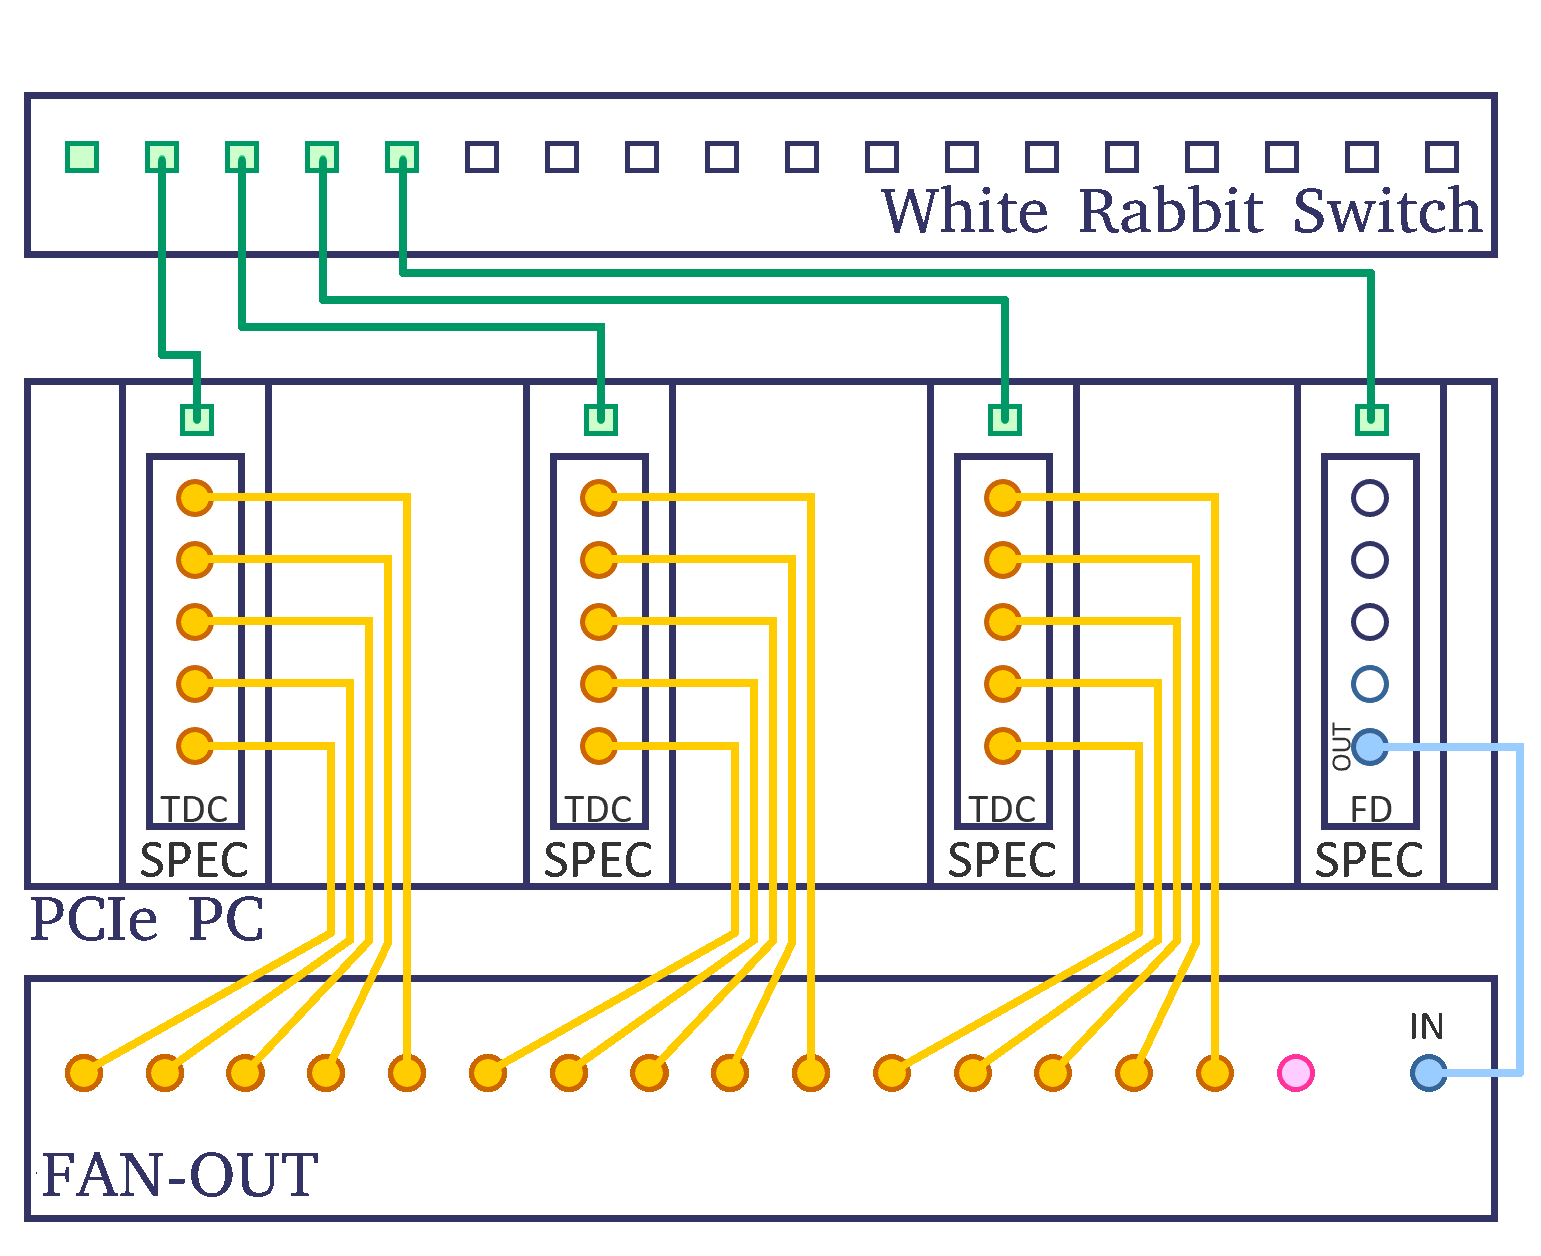
\includegraphics[width=0.6\textwidth]{img/TDC-setup_SPEC.png}
  \caption{SPEC test setup}
  \label{SPEC_test_setup_fig}
\end{figure}

The PC machine used to host SPEC cards is Siemens IPC847E with
Intel Core i5-8500\cite{spec.cpu} CPU and 8GB of RAM.
The CPU has 6-cores, no hyper-threading, with base frequency 3GHz,
maximum 4.1GHz.
The tests were run on CentOS~7 with the Linux kernel
3.10.0-957.1.3.rt56.913.el7.x86\_64 with Preempt RT patches.

~

\FloatBarrier

\section{SVEC Tests}
\label{svec_tests}

The VME crate used for testing consists one SVEC carrier populated with two
FMC-TDC. The Fine-Delay generating pulses was reused from the SPEC test setup.
Like in the SPEC tests the Fine-Delay was placed on the SPEC carrier in the PC.
Channel 1 from the Fine-Delay was connected to the fanout. One output from
the fanout was connected to the channel~2 of the bottom FMC-TDC.
The figure \ref{SVEC_test_setup_fig} shows the overview of
the setup used with the SVEC carrier in a graphical form.

\begin{figure}[ht!]
  \centering
  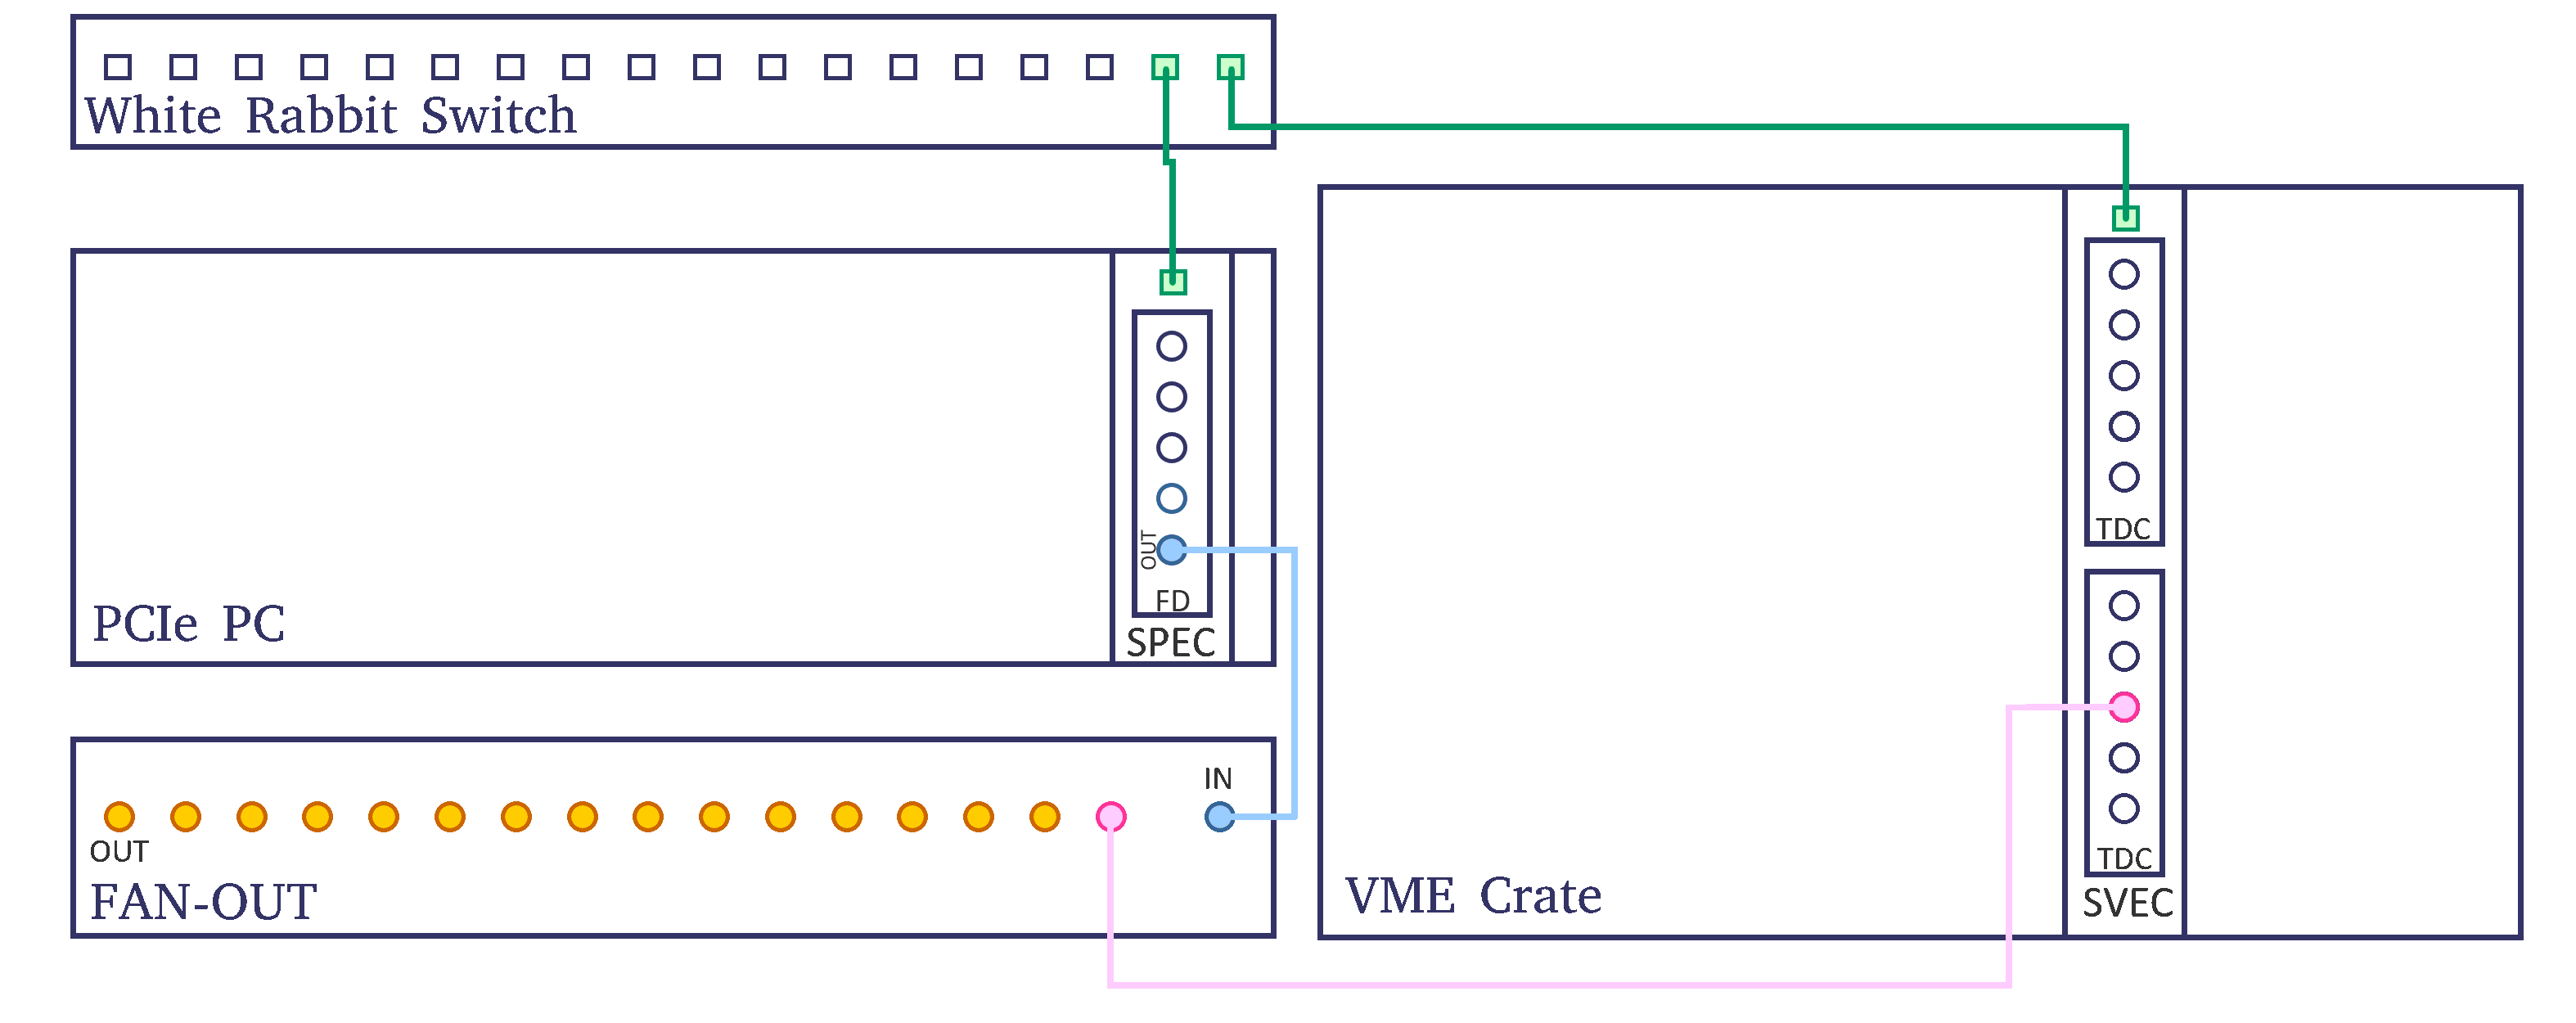
\includegraphics[width=0.95\textwidth]{img/TDC-setup_SVEC_flat.png}
  \caption{SVEC test setup}
  \label{SVEC_test_setup_fig}
\end{figure}

The used VME crate was populated with MEN A25\cite{a25} as a VME master.
It has Intel Pentium D1519\cite{svec.cpu} CPU and 8GB of RAM.
The CPU has 4-cores with hyper-threading, with base frequency 1.5GHz,
maximum 2.1GHz.
The tests were run on CentOS~7 with the Linux kernel
3.10.0-957.1.3.rt56.913.el7.x86\_64 with Preempt RT patches.

\FloatBarrier

\section{SPEC Tests}
\label{spec_tests}

\subsection{Test 1}
\label{test1}
Test summary:
\begin{center}
  \begin{tabular}{|l|l|}
    \hline {\bf Test parameter} & {\bf Value} \\
    \hline
    Pulse frequency                      & 1kHz  \\
    Pulse width                          & 1000ns \\
    Test duration                        & 27 hours \\
    Number of samples                    & 100M \\
    Clock reference                      & local \\
    \hline
  \end{tabular}
\end{center}

In this test the TDC used the local oscillator as a time reference.

\begin{figure}[ht!]
  \centering
   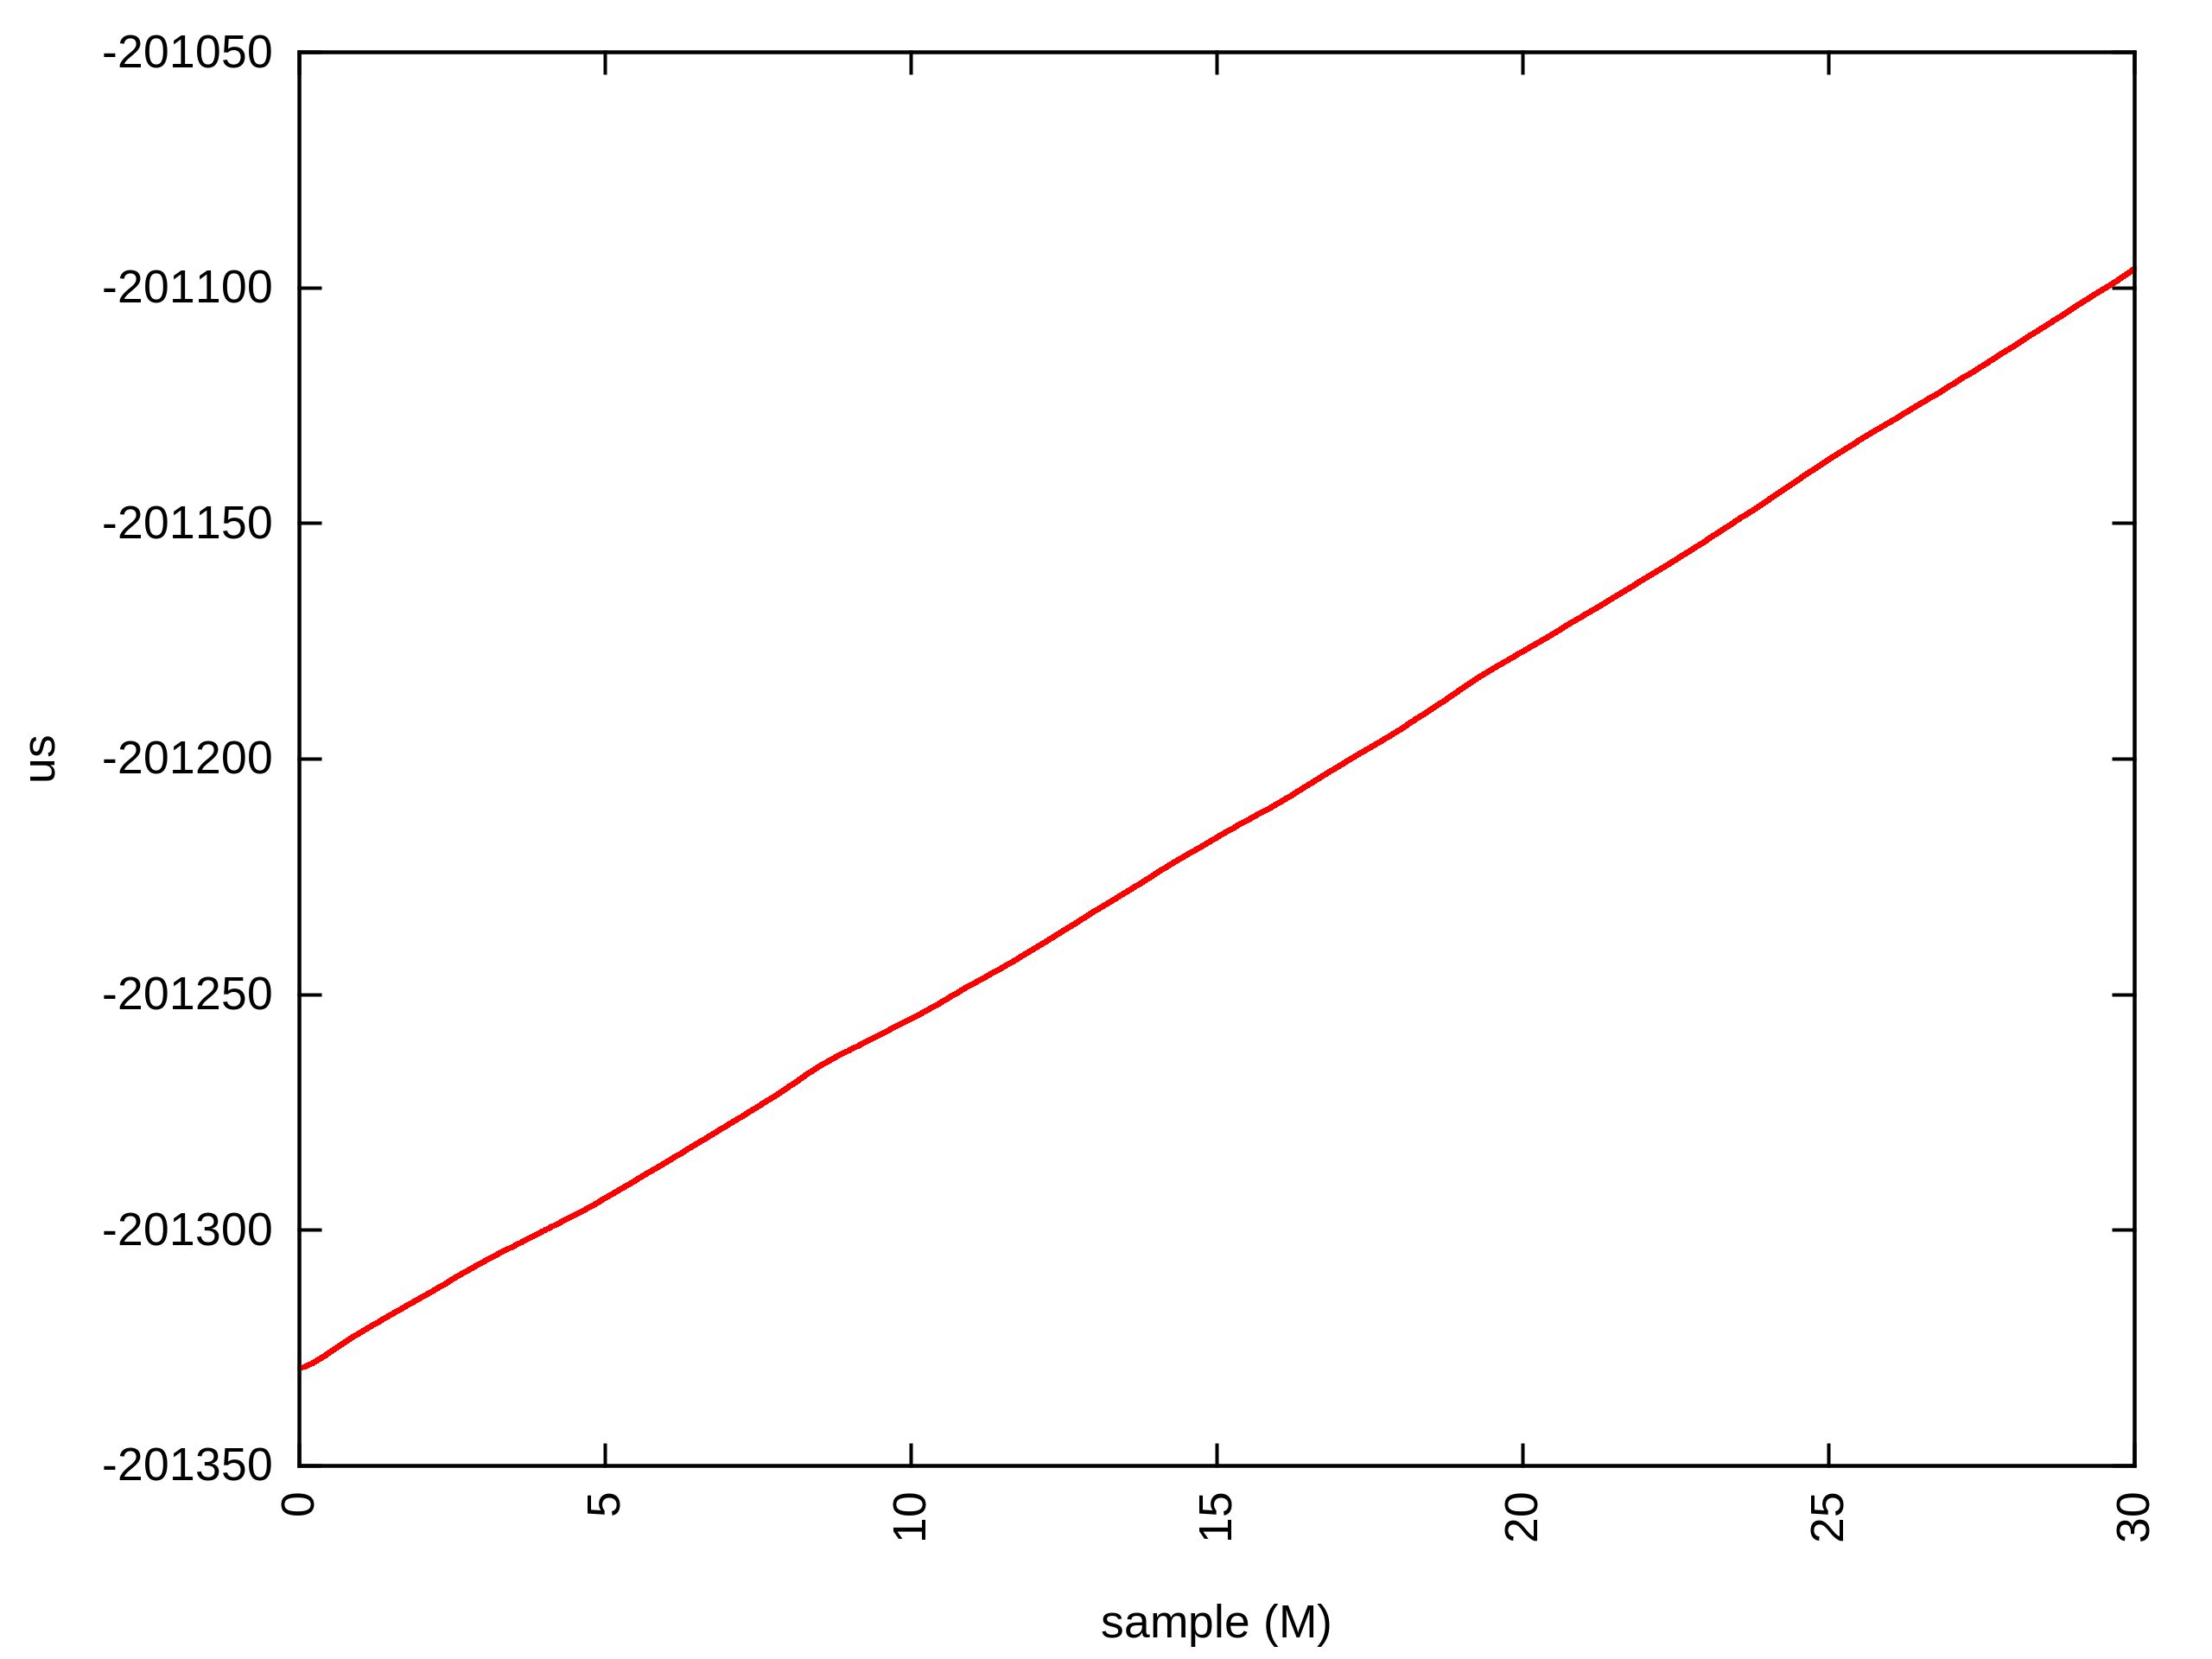
\includegraphics[width=0.80\textwidth]{img/test1_samples_absolute.png}
  \caption{Test 1: Acquired samples (absolute timestamps)}
  \label{test1_absolute}
\end{figure}

\begin{figure}[ht!]
  \centering
   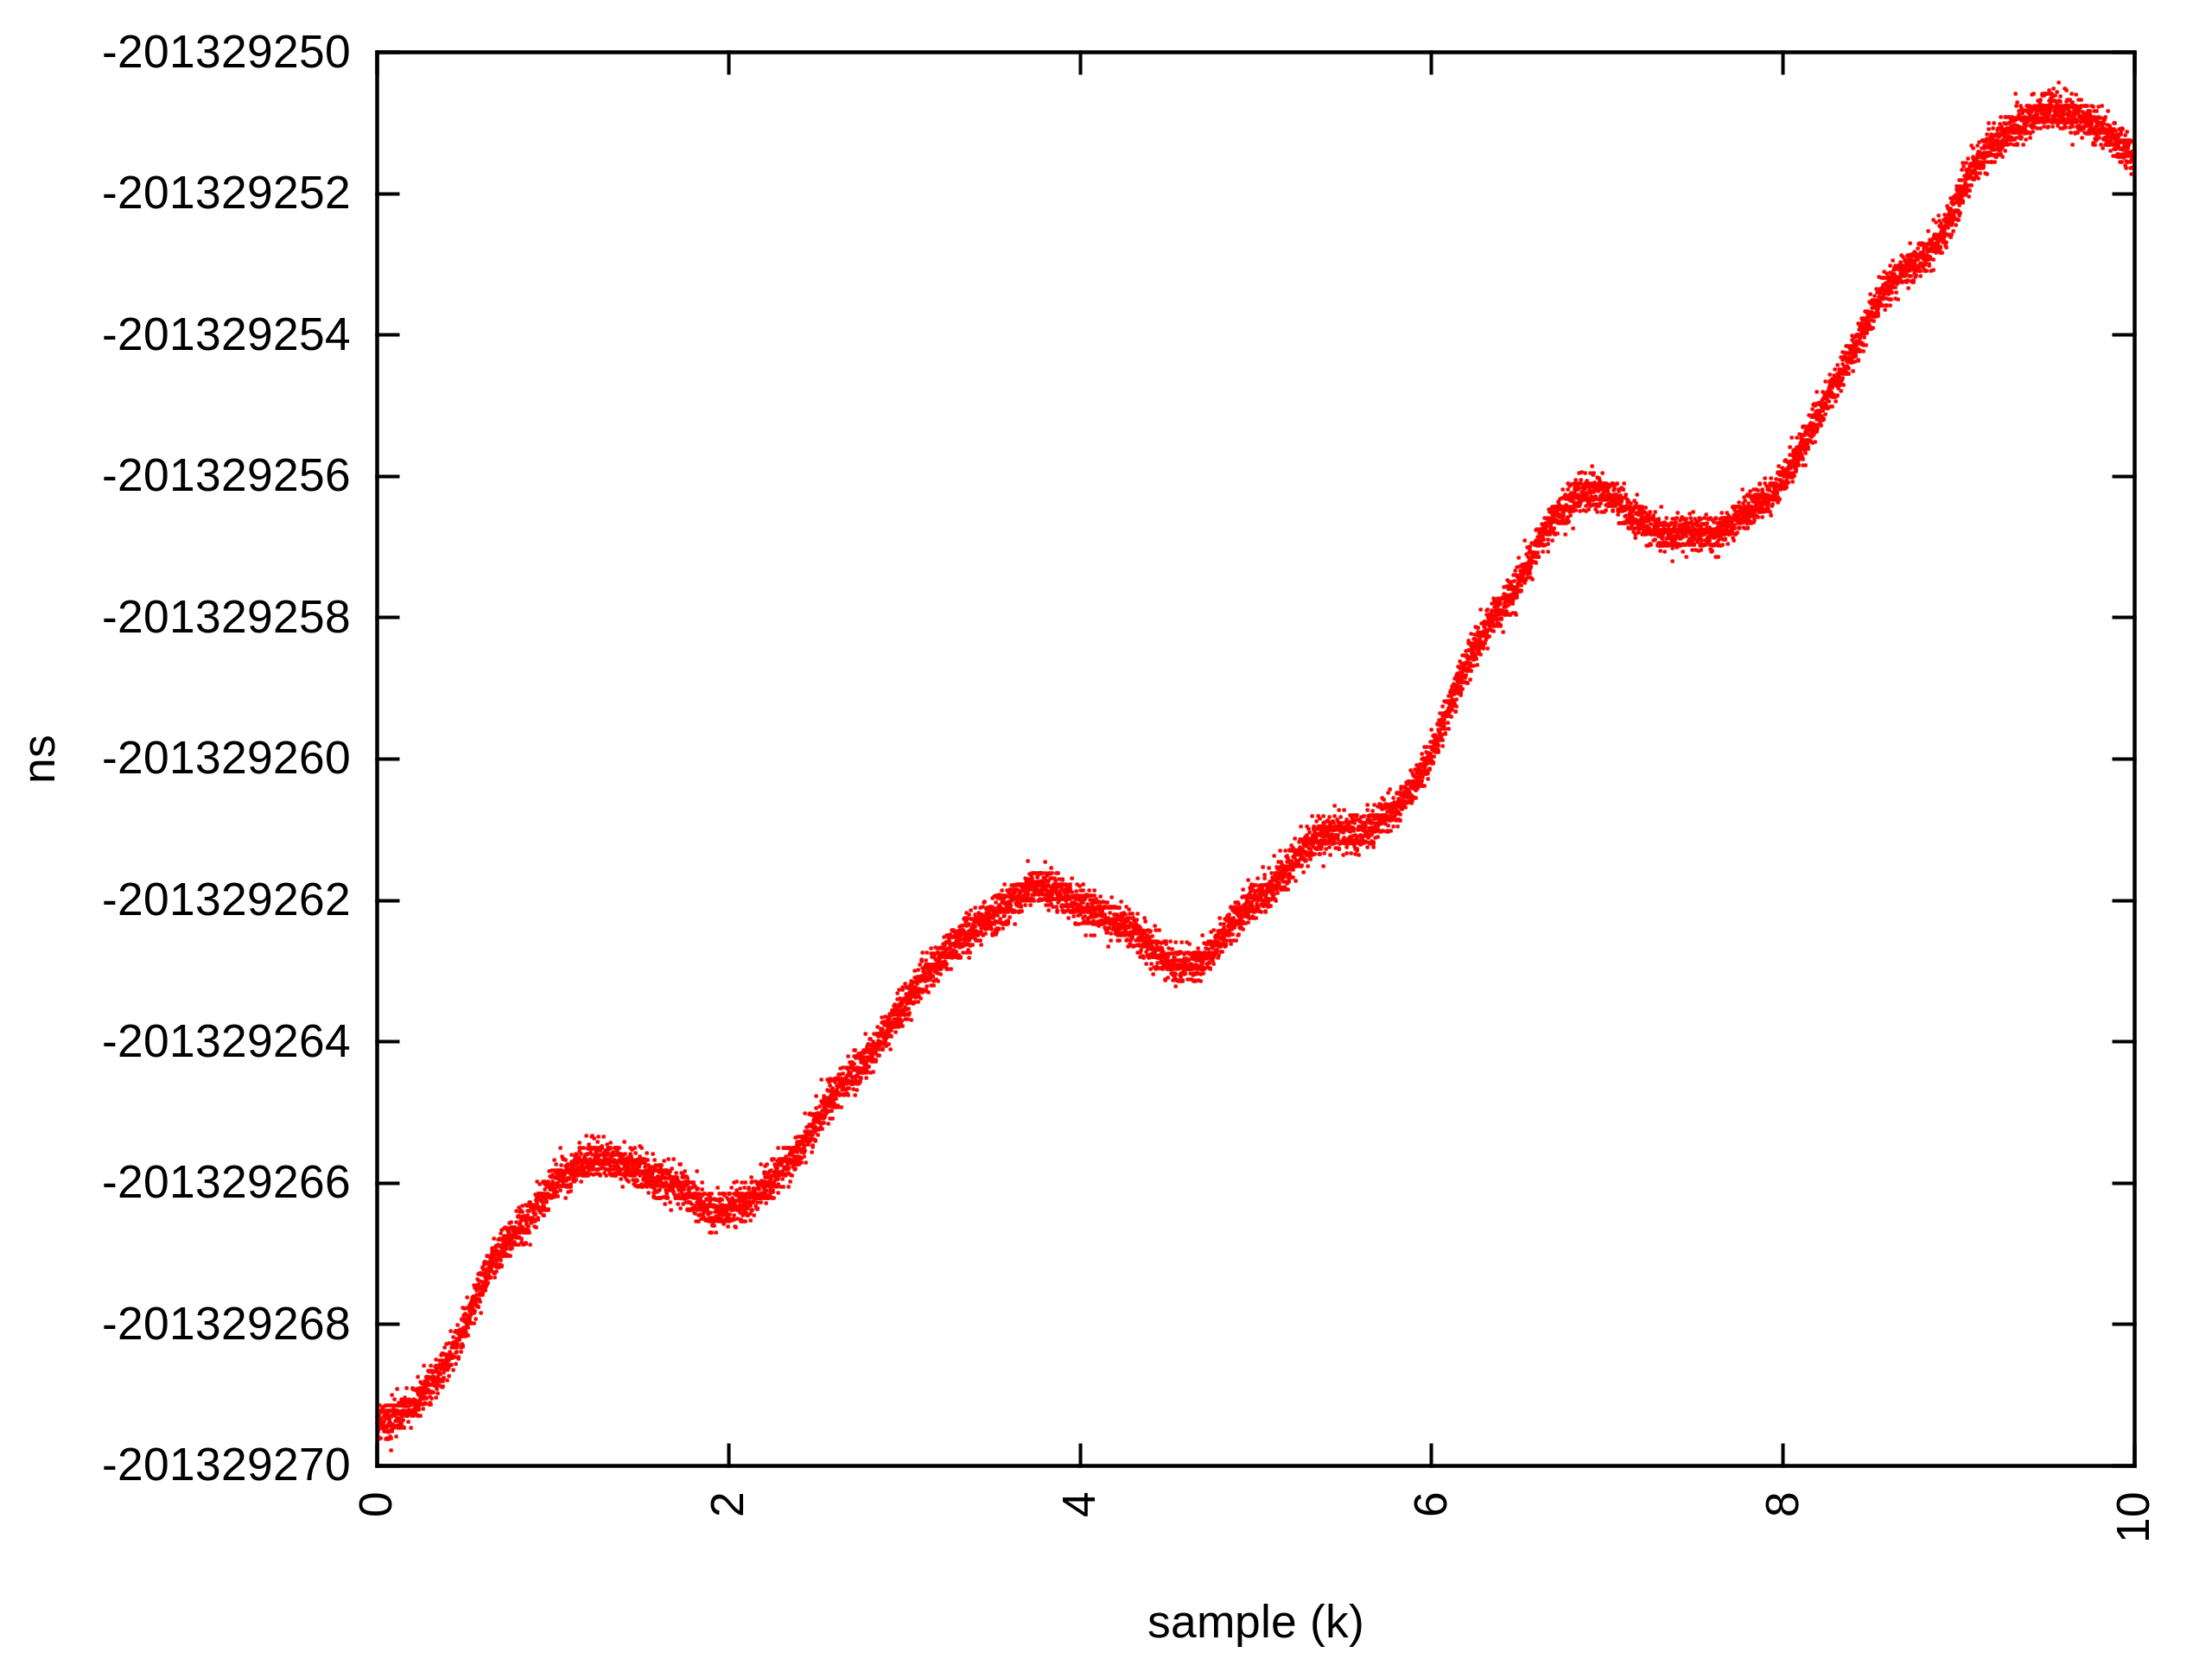
\includegraphics[width=0.80\textwidth]{img/test1_samples_absolute_zoom.png}
  \caption{Test 1: Subset of acquired samples (absolute timestamps)}
  \label{test1_absolute_zoom}
\end{figure}

Figures~\ref{test1_absolute} and~\ref{test1_absolute_zoom} show the absolute
timestamps of the data gathered during run 1 of this test.
The data presented in the~Figure~\ref{test1_absolute} shows the continuous
drift of the local oscillator from the White Rabbit used as the reference on
the Fine-Delay board generating pulses.
If there were no drift, the line in the~Figure~\ref{test1_absolute} would be
horizontal (like in~Figure~\ref{test1_absolute} of \textit{Test~2}).
Additionally, it can be observed that the line in the
Figure~\ref{test1_absolute} is not straight.
This is caused by the fluctuations of the drift of the local oscillator
compared to the White Rabbit.
Figure~\ref{test1_absolute_zoom} is the zoom in of the the data presented in
the~Figure~\ref{test1_absolute}. It shows in details the mentioned fluctuations.

\FloatBarrier

\begin{figure}[ht!]
  \centering
  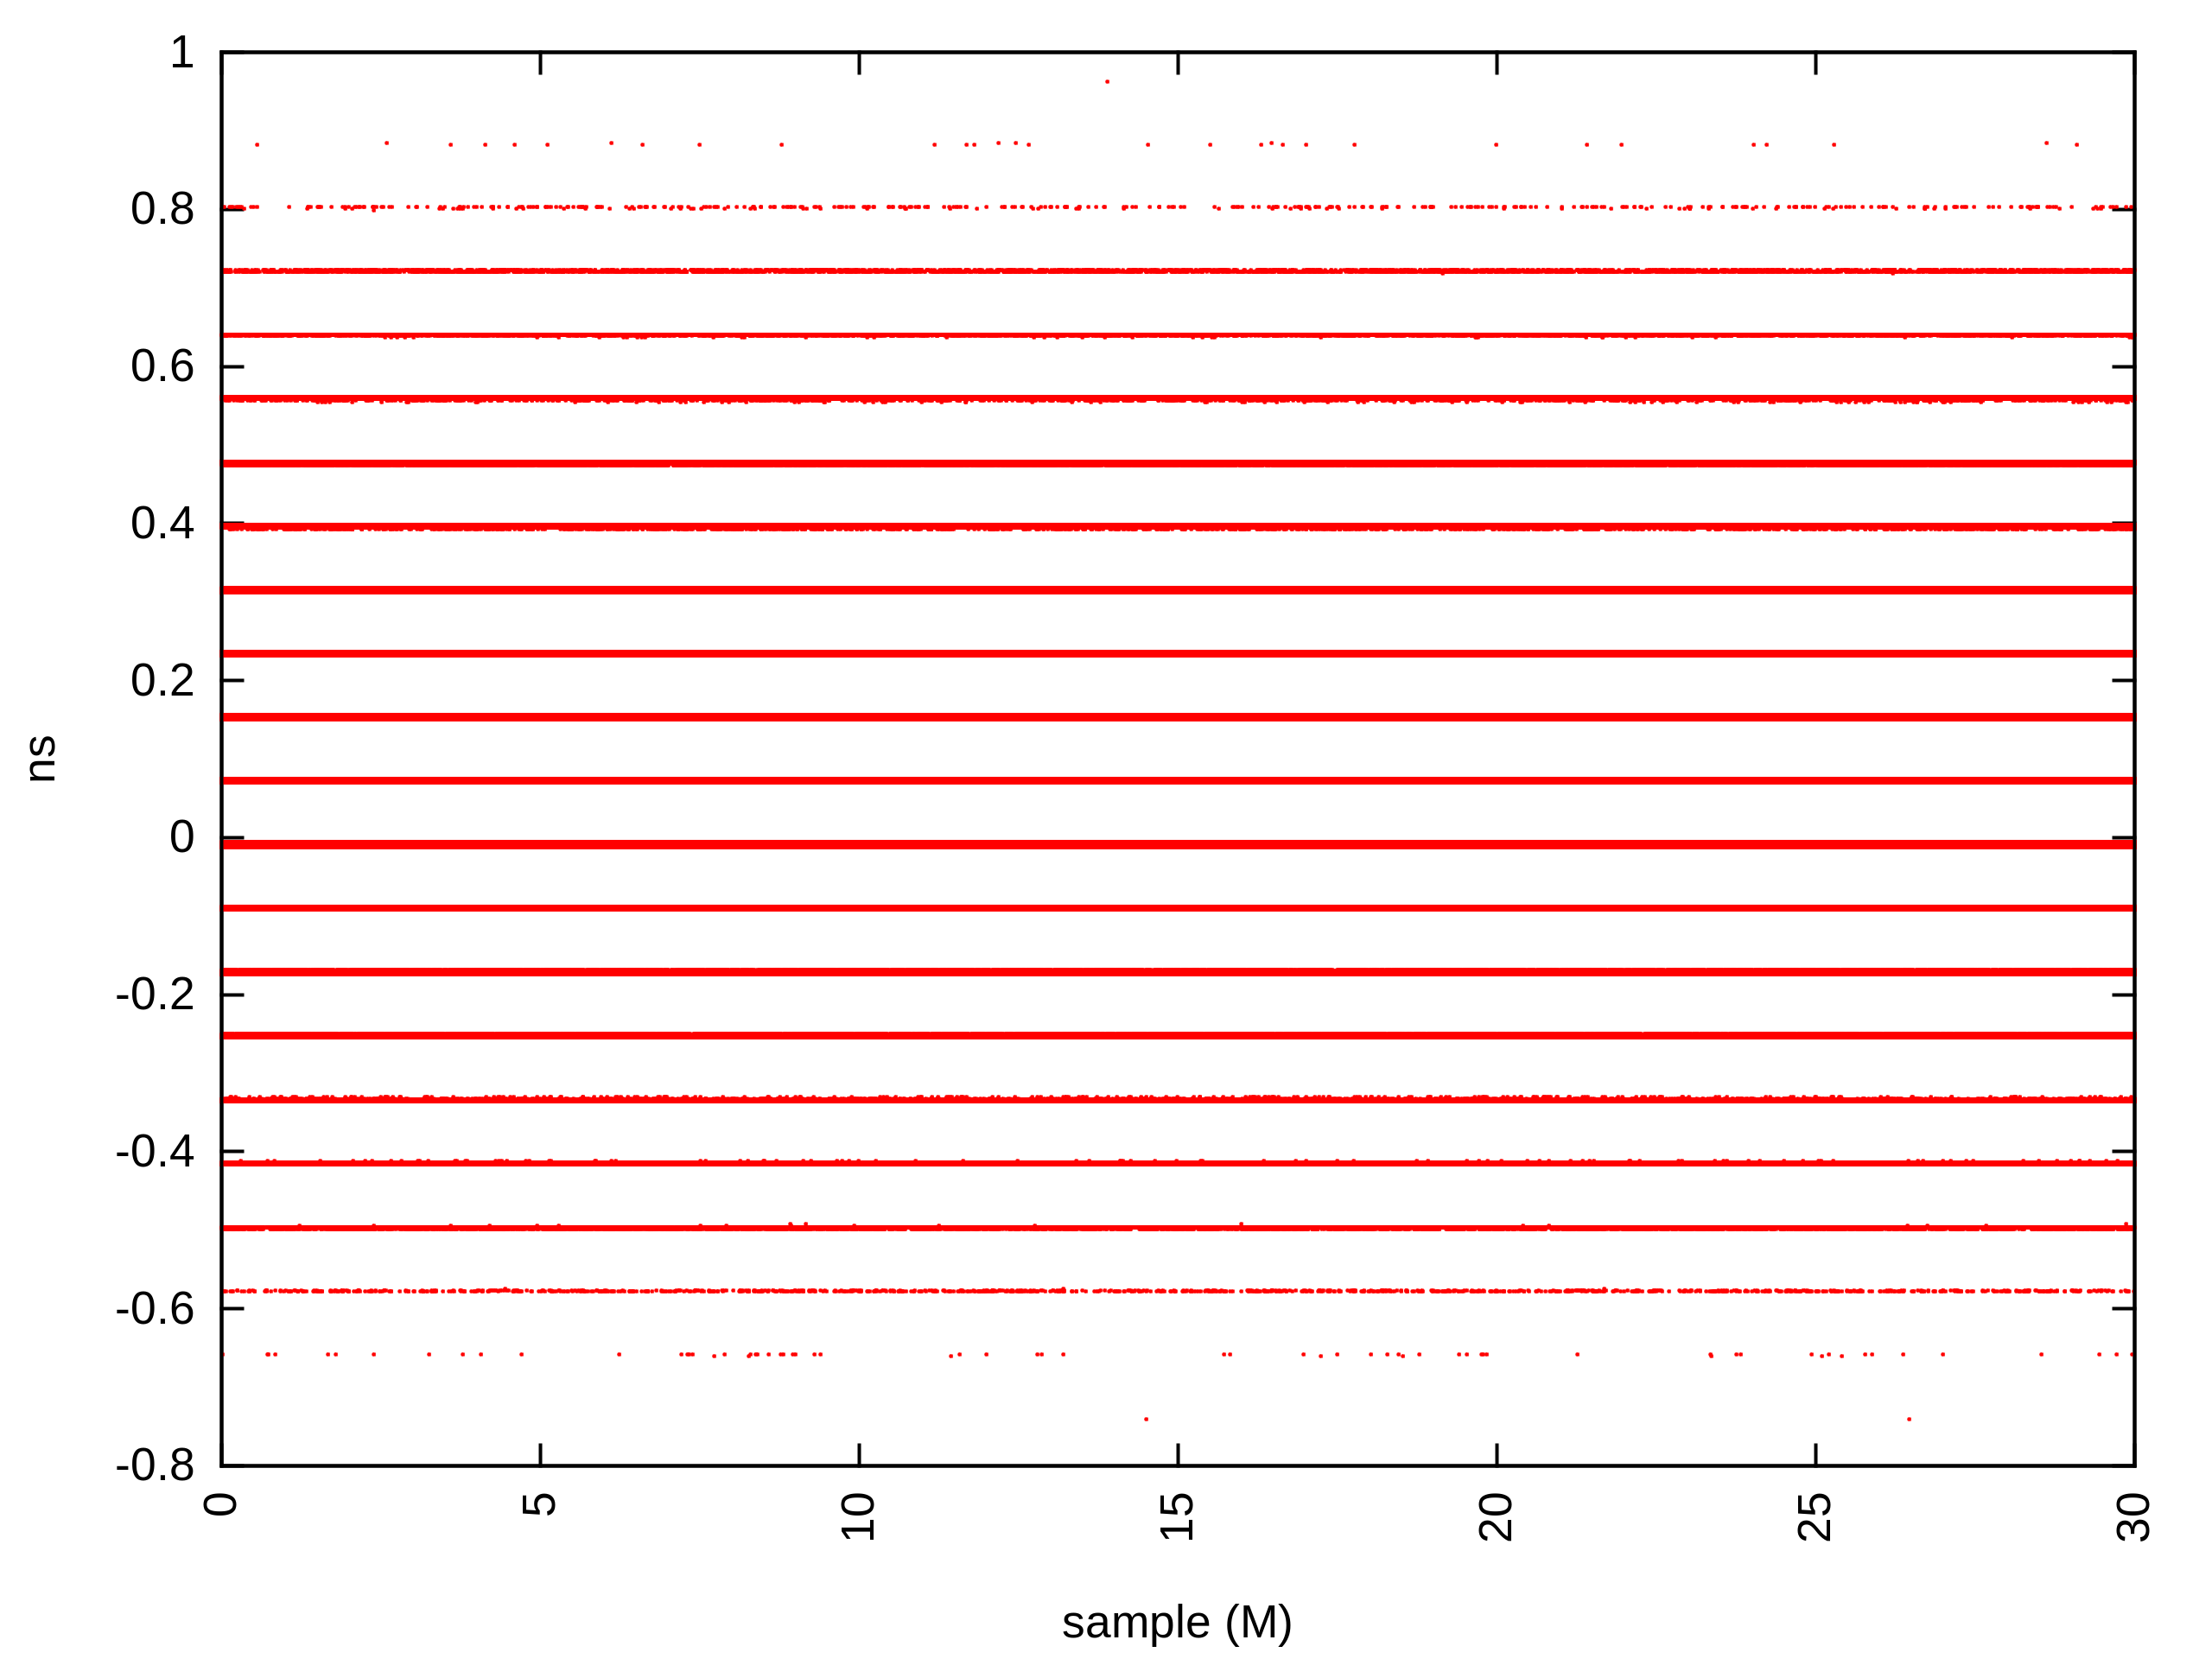
\includegraphics[width=0.7\textwidth]{img/test1_samples_relative.png}
  \caption{Test 1: Acquired samples (relative timestamps)}
  \label{test1_relative}
\end{figure}

\begin{figure}[ht!]
  \centering
  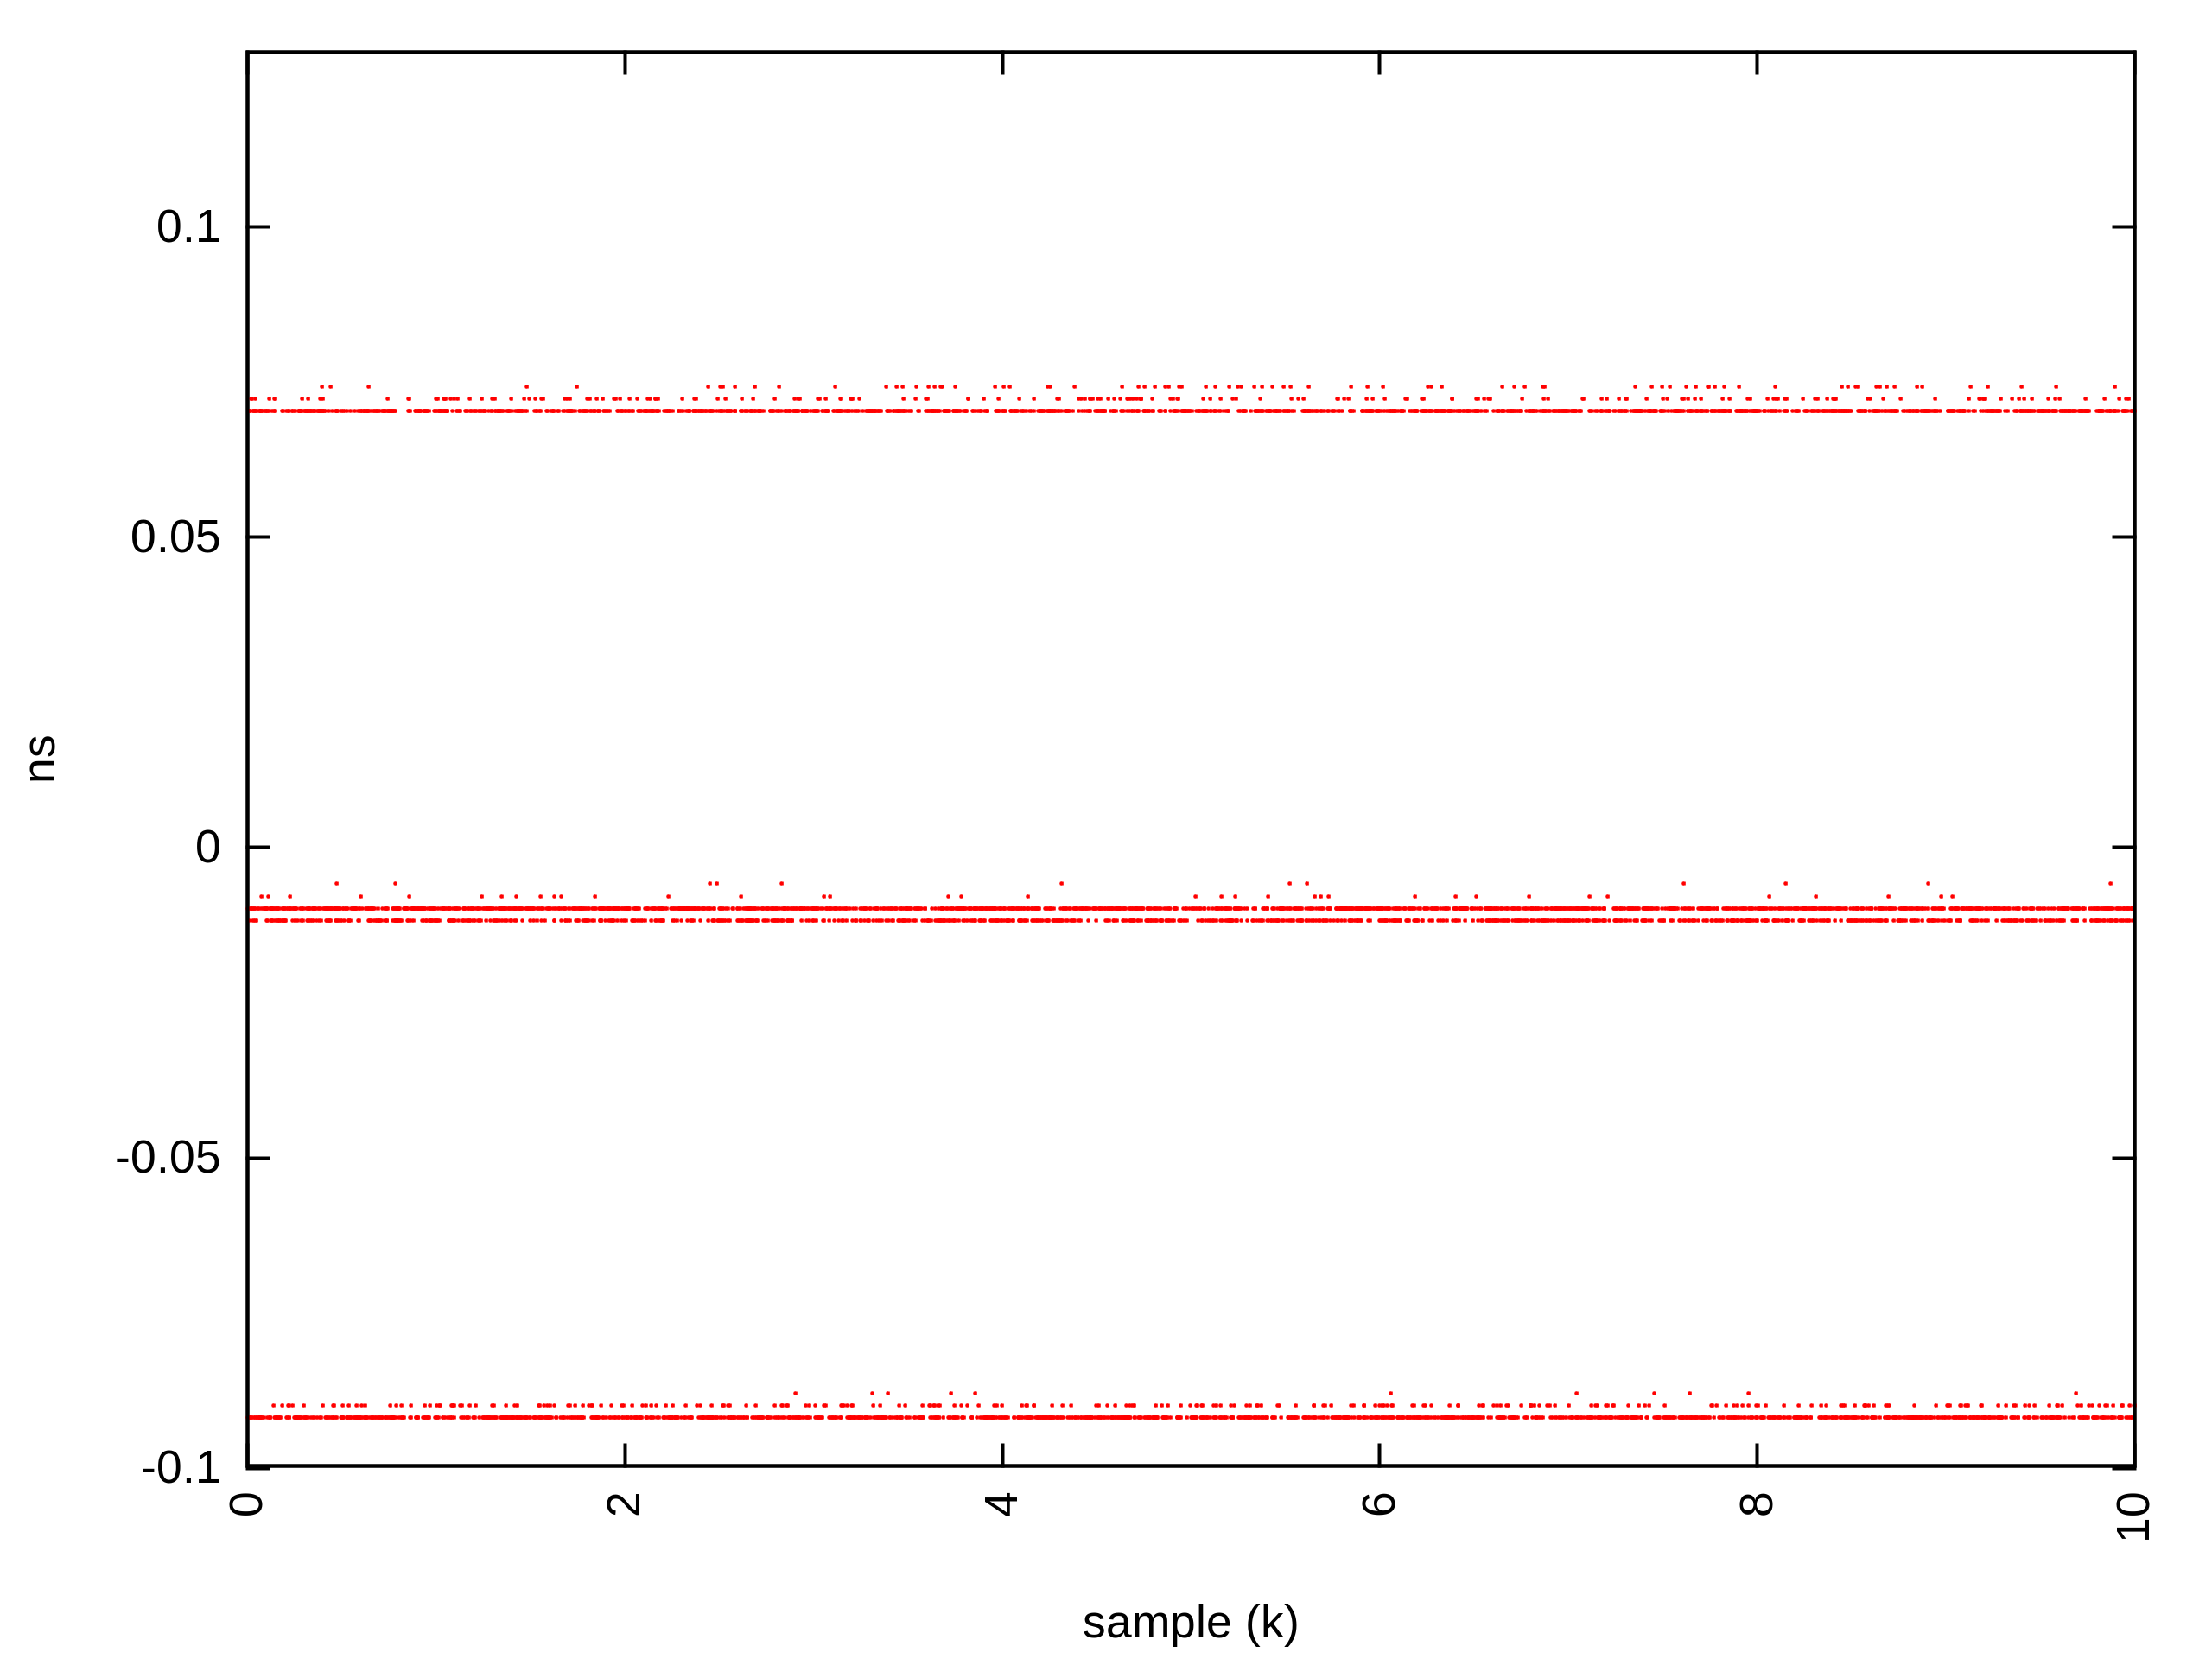
\includegraphics[width=0.7\textwidth]{img/test1_samples_relative_zoomxy.png}
  \caption{Test 1: Subset of acquired samples (relative timestamps)}
  \label{test1_relative_zoomy}
\end{figure}

The~Figure~\ref{test1_relative} shows the relative timestamps of the acquired
data.
Relative timestamps are arranged as several horizontal lines.
It is believed that this quantization is due to the internal architecture of
the timestamping chip used on the TDC.
Zooming the data presented in the~Figure~\ref{test1_relative}, shows that each
line contains samples at few levels (Figure~\ref{test1_relative_zoomy}).

\FloatBarrier

\begin{figure}[ht!]
  \centering
  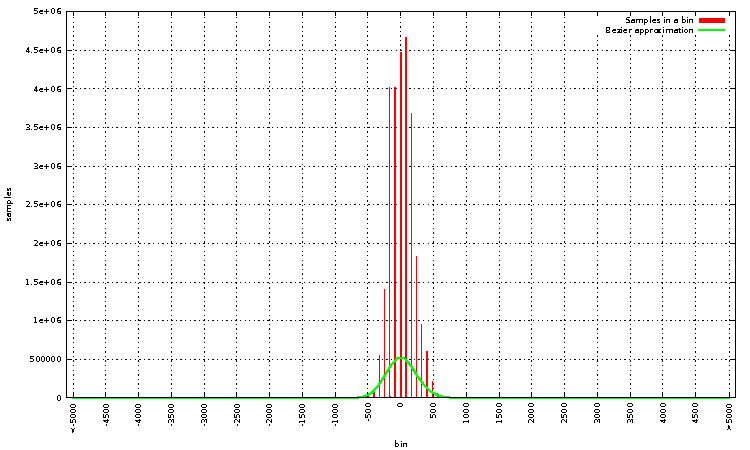
\includegraphics[width=0.80\textwidth]{img/test1_histogram.pdf}
  \caption{Test 1: Histogram of acquired samples (relative timestamps)}
  \label{test1_histogram}
\end{figure}

The same relative samples as above are
presented in the form of histogram in the~Figure~\ref{test1_histogram}.
The histogram is divided into 1000 bins.
Each bin spans over 10 ps.
Two additional bins were added to keep all values greater and smaller than
5000ps.

As a consequence of the distribution of samples shown in
the~Figure~\ref{test1_relative}, there are many empty bins between filled bins
(like gaps between lines in the mentioned figure).
To overcome quantization effect and to give better overview
the Bezier approximation has been added to the histogram figure.

\begin{figure}[ht!]
  \centering
  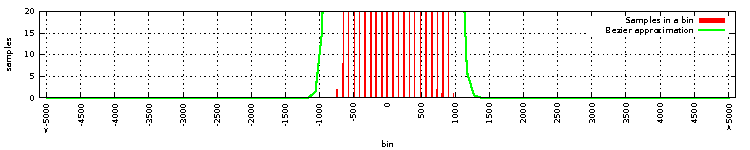
\includegraphics[width=1\textwidth]{img/test1_histogram_zoomy.pdf}
  \caption{Test 1: Histogram of acquired samples (relative timestamps),
           zoom in on the Y axis of the histogram (Figure~\ref{test1_histogram})}
  \label{test1_histogram_zoomy}
\end{figure}

Figure~\ref{test1_histogram_zoomy} shows the zoom in on the Y axis of the histogram
presented in the~Figure~\ref{test1_histogram}. This shows that all bins outside
the center part of the figure are empty.
The Bezier curve may suggest that there are samples outside the range
-750ps to 1000ps, but all these bins are empty.
This effect is due to the way how the Bezier curve is calculated.

\begin{figure}[ht!]
  \centering
  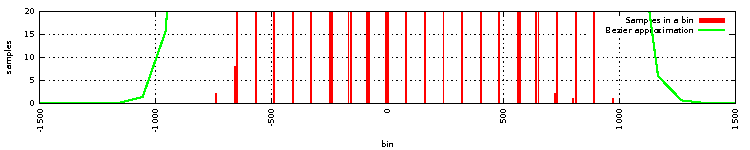
\includegraphics[width=1\textwidth]{img/test1_histogram_zoomx.pdf}
  \caption{Test 1: Histogram of acquired samples (relative timestamps), zoom in
	   of the bottom center part of the histogram
	   (Figure~\ref{test1_histogram})}
  \label{test1_histogram_zoomx}
\end{figure}

Figure~\ref{test1_histogram_zoomx} shows the zoom in of the bottom center part
of the histogram presented in the~Figure~\ref{test1_histogram}.
It gives a better view about the presence of samples in bins that are close to
the center of the histogram.

\FloatBarrier

\begin{table}[!htb]
  \centering
  \footnotesize
  \begin{tabular}{|c|r|r|r|r|r|r|}
    \hline {\bf Run} & {\bf Data Volume} & {\bf Mean (ps)} & {\bf Sigma (ps)} & {\bf Min (ps)} & {\bf Max (ps)} & {\bf Range (ps)}  \\
    \hline
    1                &  30M              &  7.780          & 164.698          & -740.234       & 962.891        &  1703.125           \\
    2                &   1M              &  4.339          & 165.741          & -658.203       & 964.844        &  1623.047           \\
    3                & 100M              & -2.148          & 164.342          & -740.234       & 962.891        &  1703.125           \\
    4                &  30M              & -0.780          & 160.717          & -740.234       & 884.766        &  1625.000           \\
    \hline
  \end{tabular}
  \caption{Summary of \textit{Test~1} relative timestamps for multiple runs}
  \label{table_test1_summary}
\end{table}

The statistical summary of several runs of the \textit{Test~1} is presented in
the Table~\ref{table_test1_summary}.
The mean value of samples within a run differs between runs due to the drift
of the local oscillator with the reference to White Rabbit used on
the pulse generator. The other values seam to be stable between different
runs.
There were runs of \textit{Test 1}, that included samples with an offset
around 4ns. However, such runs were not included in the table above..

To gather all data in the described test, the following python command has been used:
\begin{lstlisting}
$ python -d -m pytest test_fmctdc_acquisition.py::TestFmctdcAcquisition::\
  test_acq_timestamp_multiple_hist --usr-acq-count=100000000
  --usr-acq-period-ns=1000000 --tdc-id-ch 0x17:1 --fd-id-ch 0x1a:1 \
  --samples-file test1 --histogram-file test1_hist \
  --bin-min-ps -5000 --bin-max-ps 5000 --bins-num 1000 --tdc-wr-off
\end{lstlisting}

\FloatBarrier

\subsection{Test 2}
\label{test2}
Test summary:
\begin{center}
  \begin{tabular}{|l|l|}
    \hline {\bf Test parameter} & {\bf Value} \\
    \hline
    Pulse frequency                      & 1kHz  \\
    Pulse width                          & 1000ns \\
    Test duration                        & 27 hours \\
    Number of samples                    & 100M \\
    Clock reference                      & White Rabbit \\
    \hline
  \end{tabular}
\end{center}
\textit{Test~2} is very similar to the~\textit{Test~1} described in
subsection~\ref{test1}.
However, in this test the TDC uses White Rabbit as a time reference
instead of the local oscillator.

\begin{figure}[ht!]
  \centering
  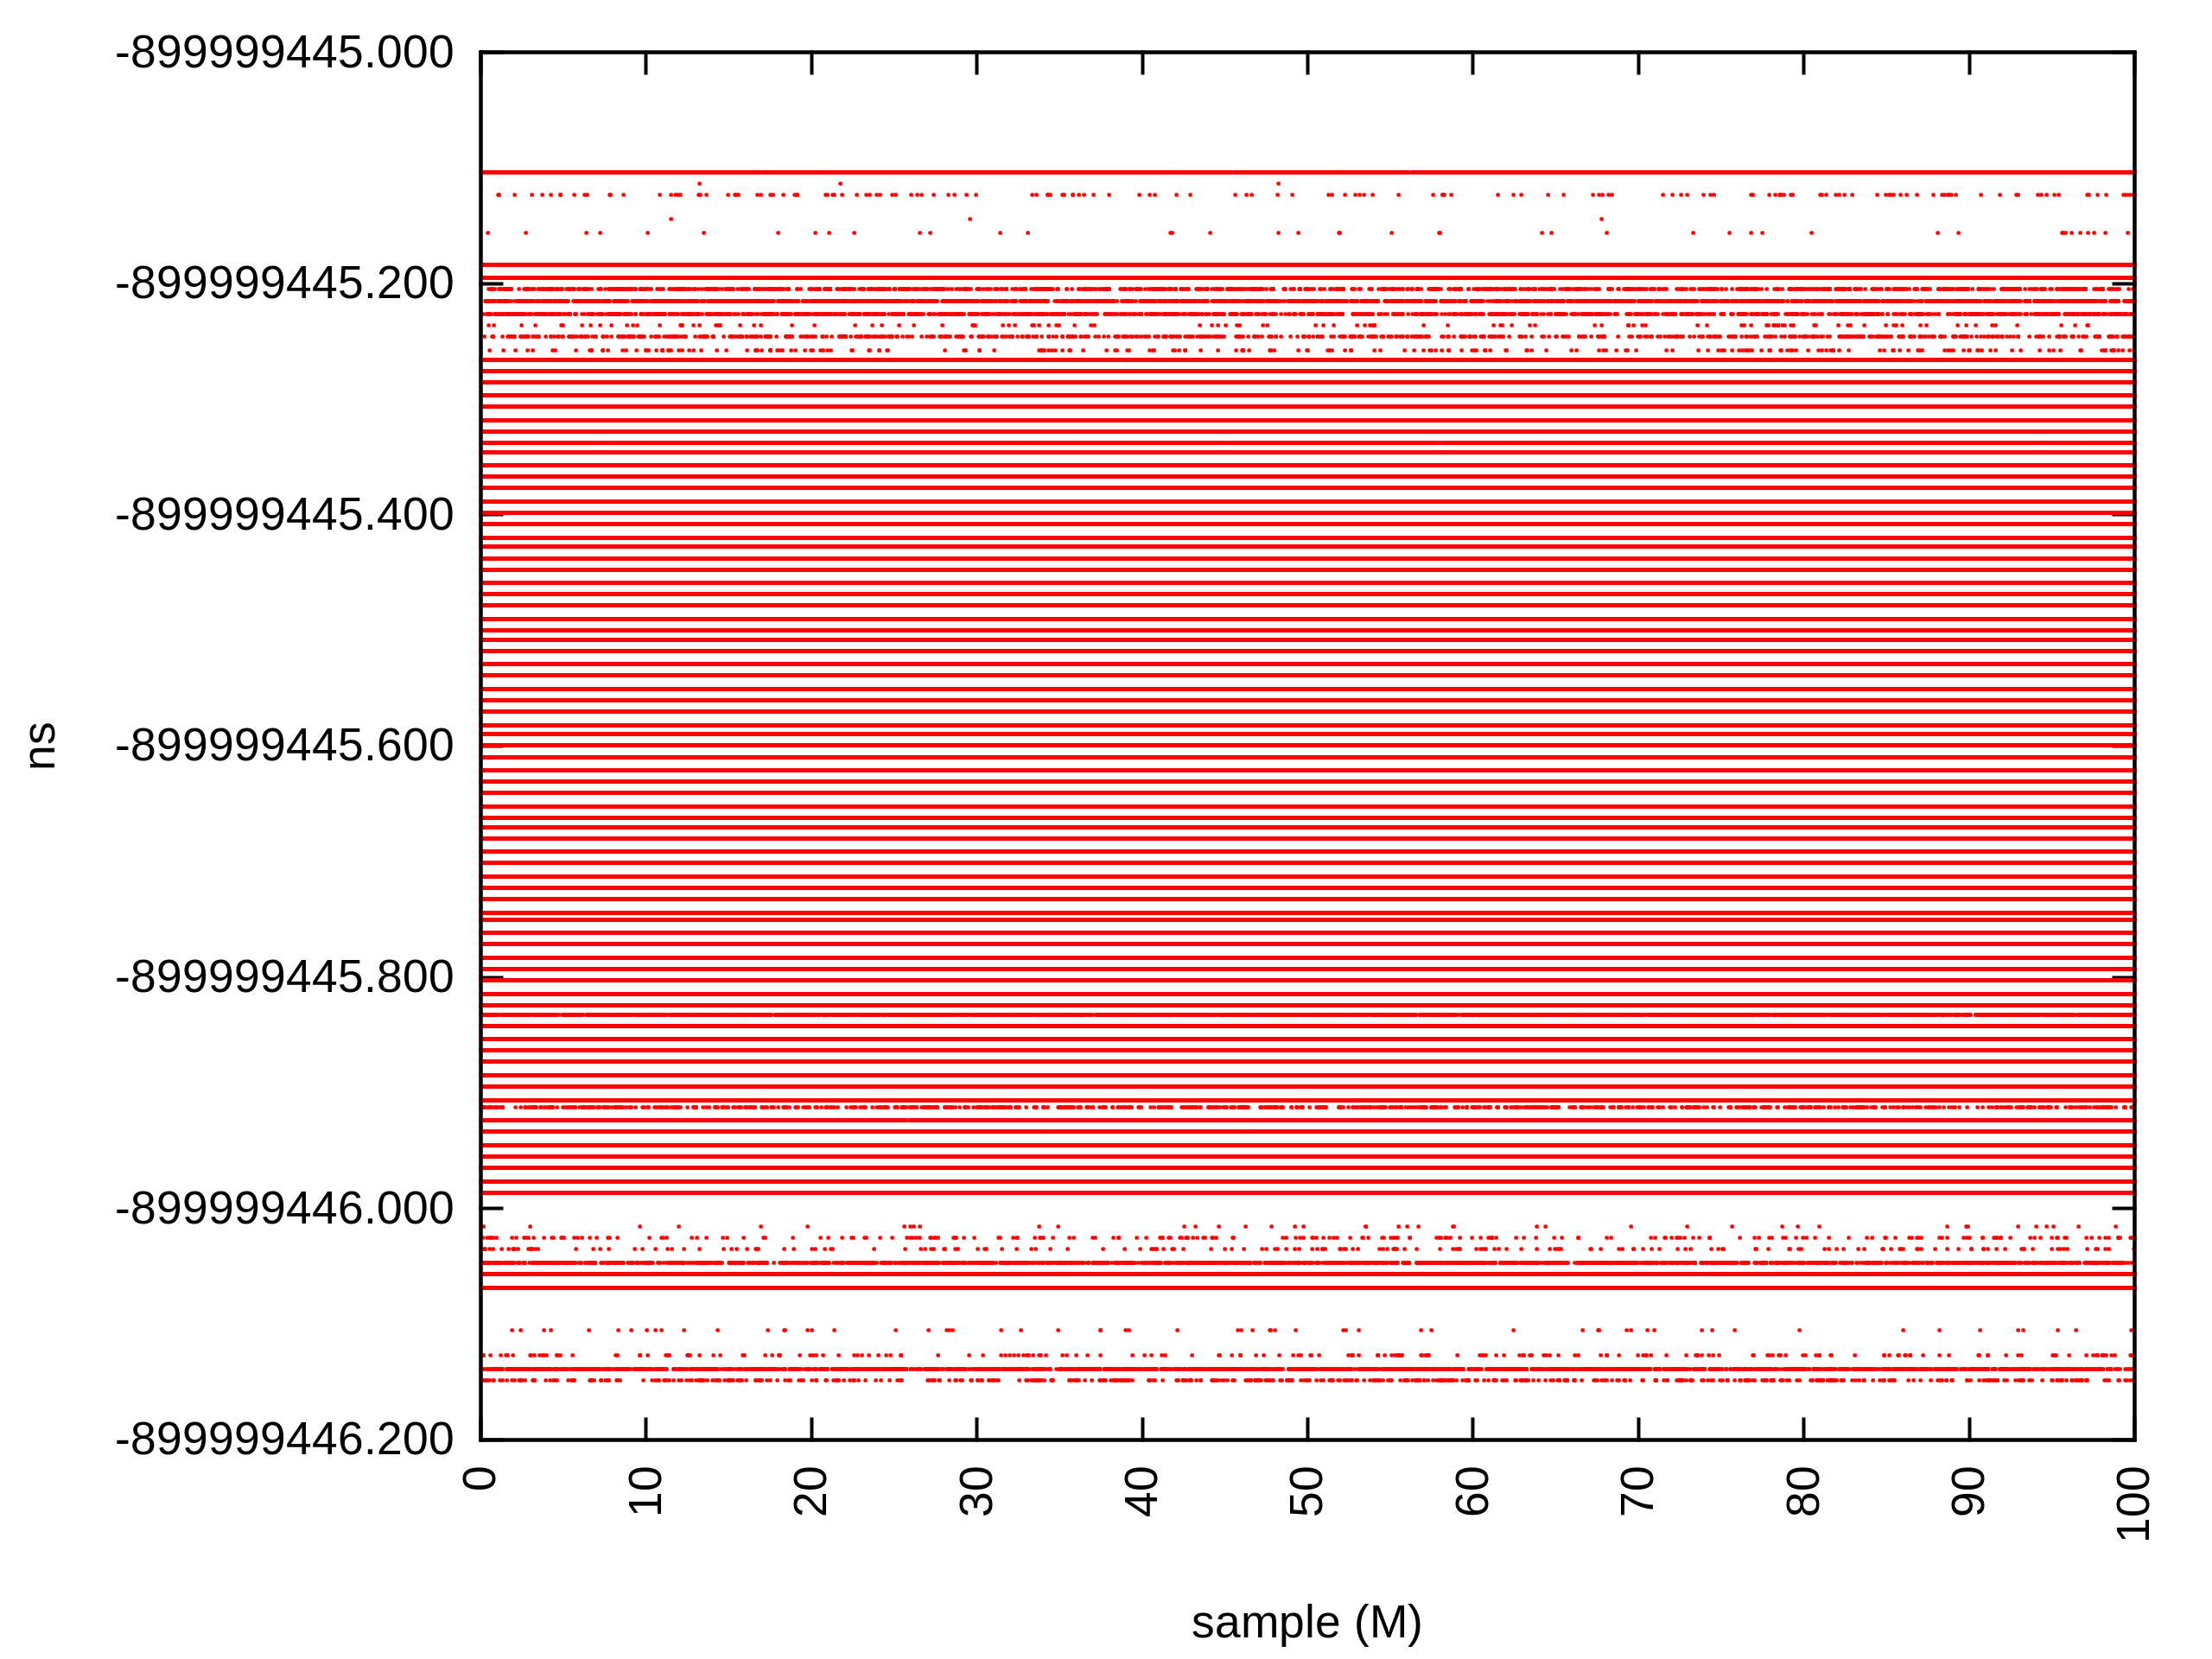
\includegraphics[width=0.80\textwidth]{img/test2_samples_absolute.png}
  \caption{Test 2: Acquired samples (absolute timestamps)}
  \label{test2_absolute}
\end{figure}

\begin{figure}[ht!]
  \centering
  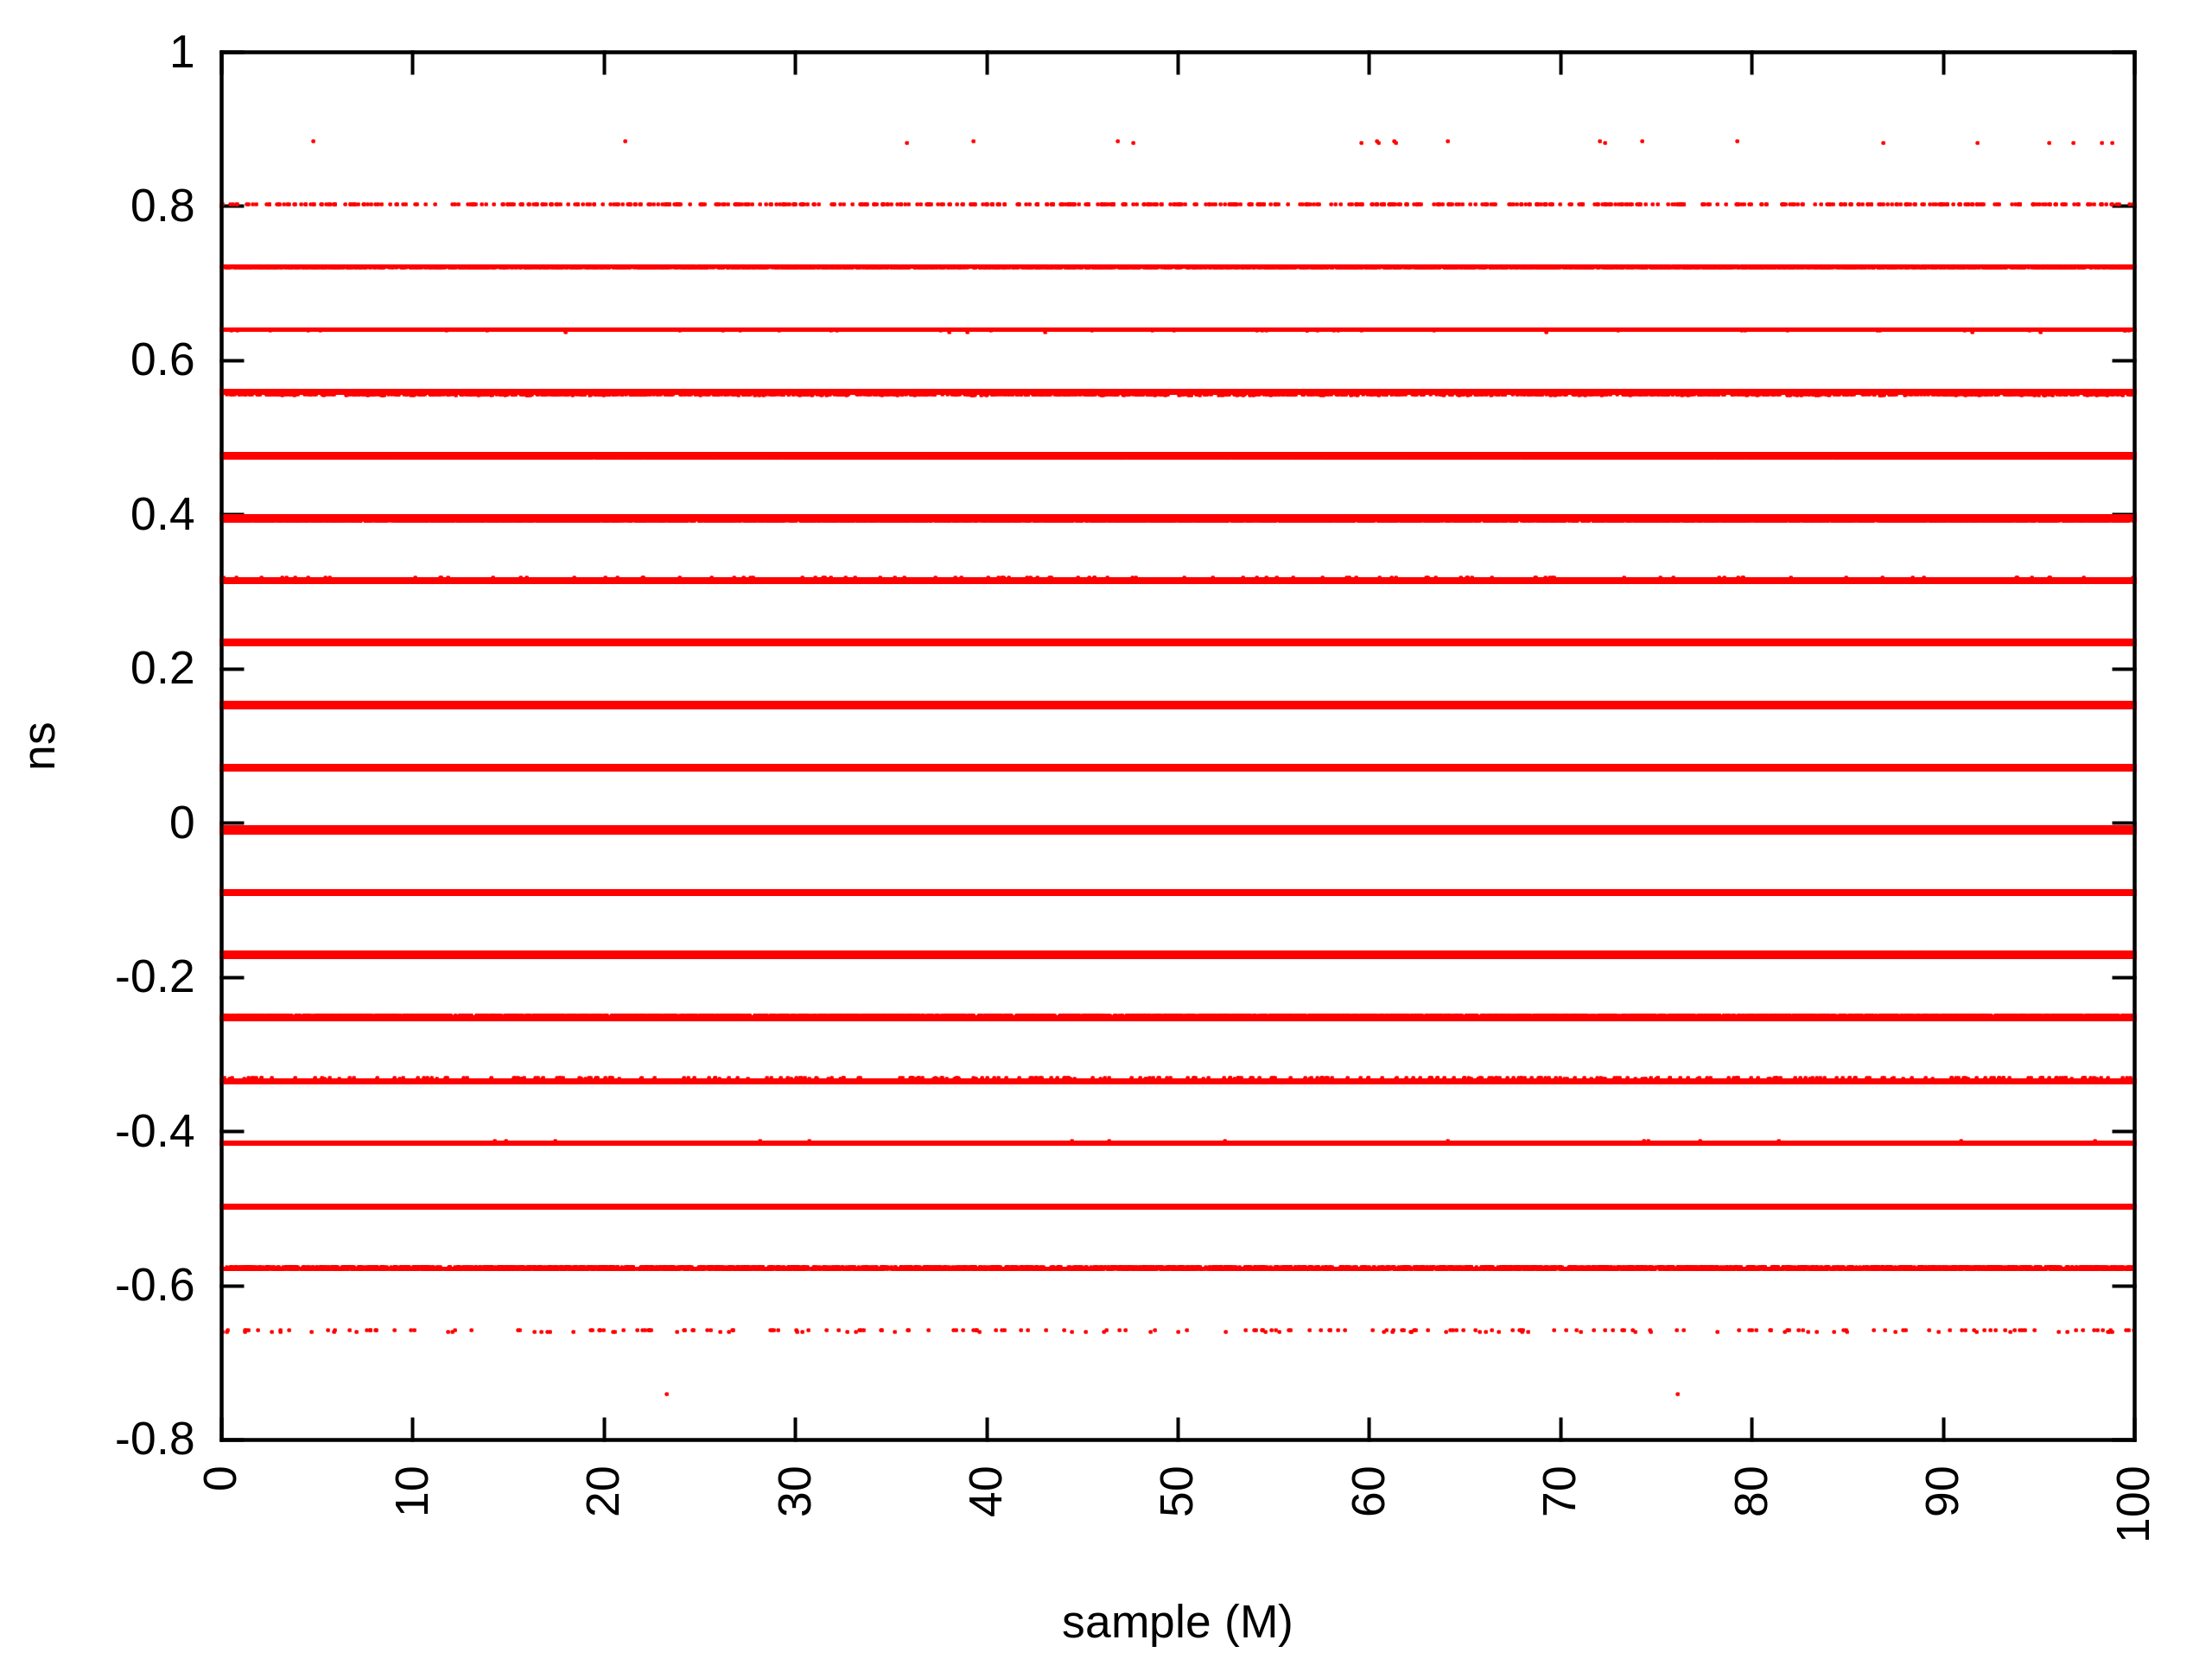
\includegraphics[width=0.9\textwidth]{img/test2_samples_relative.png}
  \caption{Test 2: Acquired samples (relative timestamps)}
  \label{test2_relative}
\end{figure}

\begin{figure}[ht!]
  \centering
  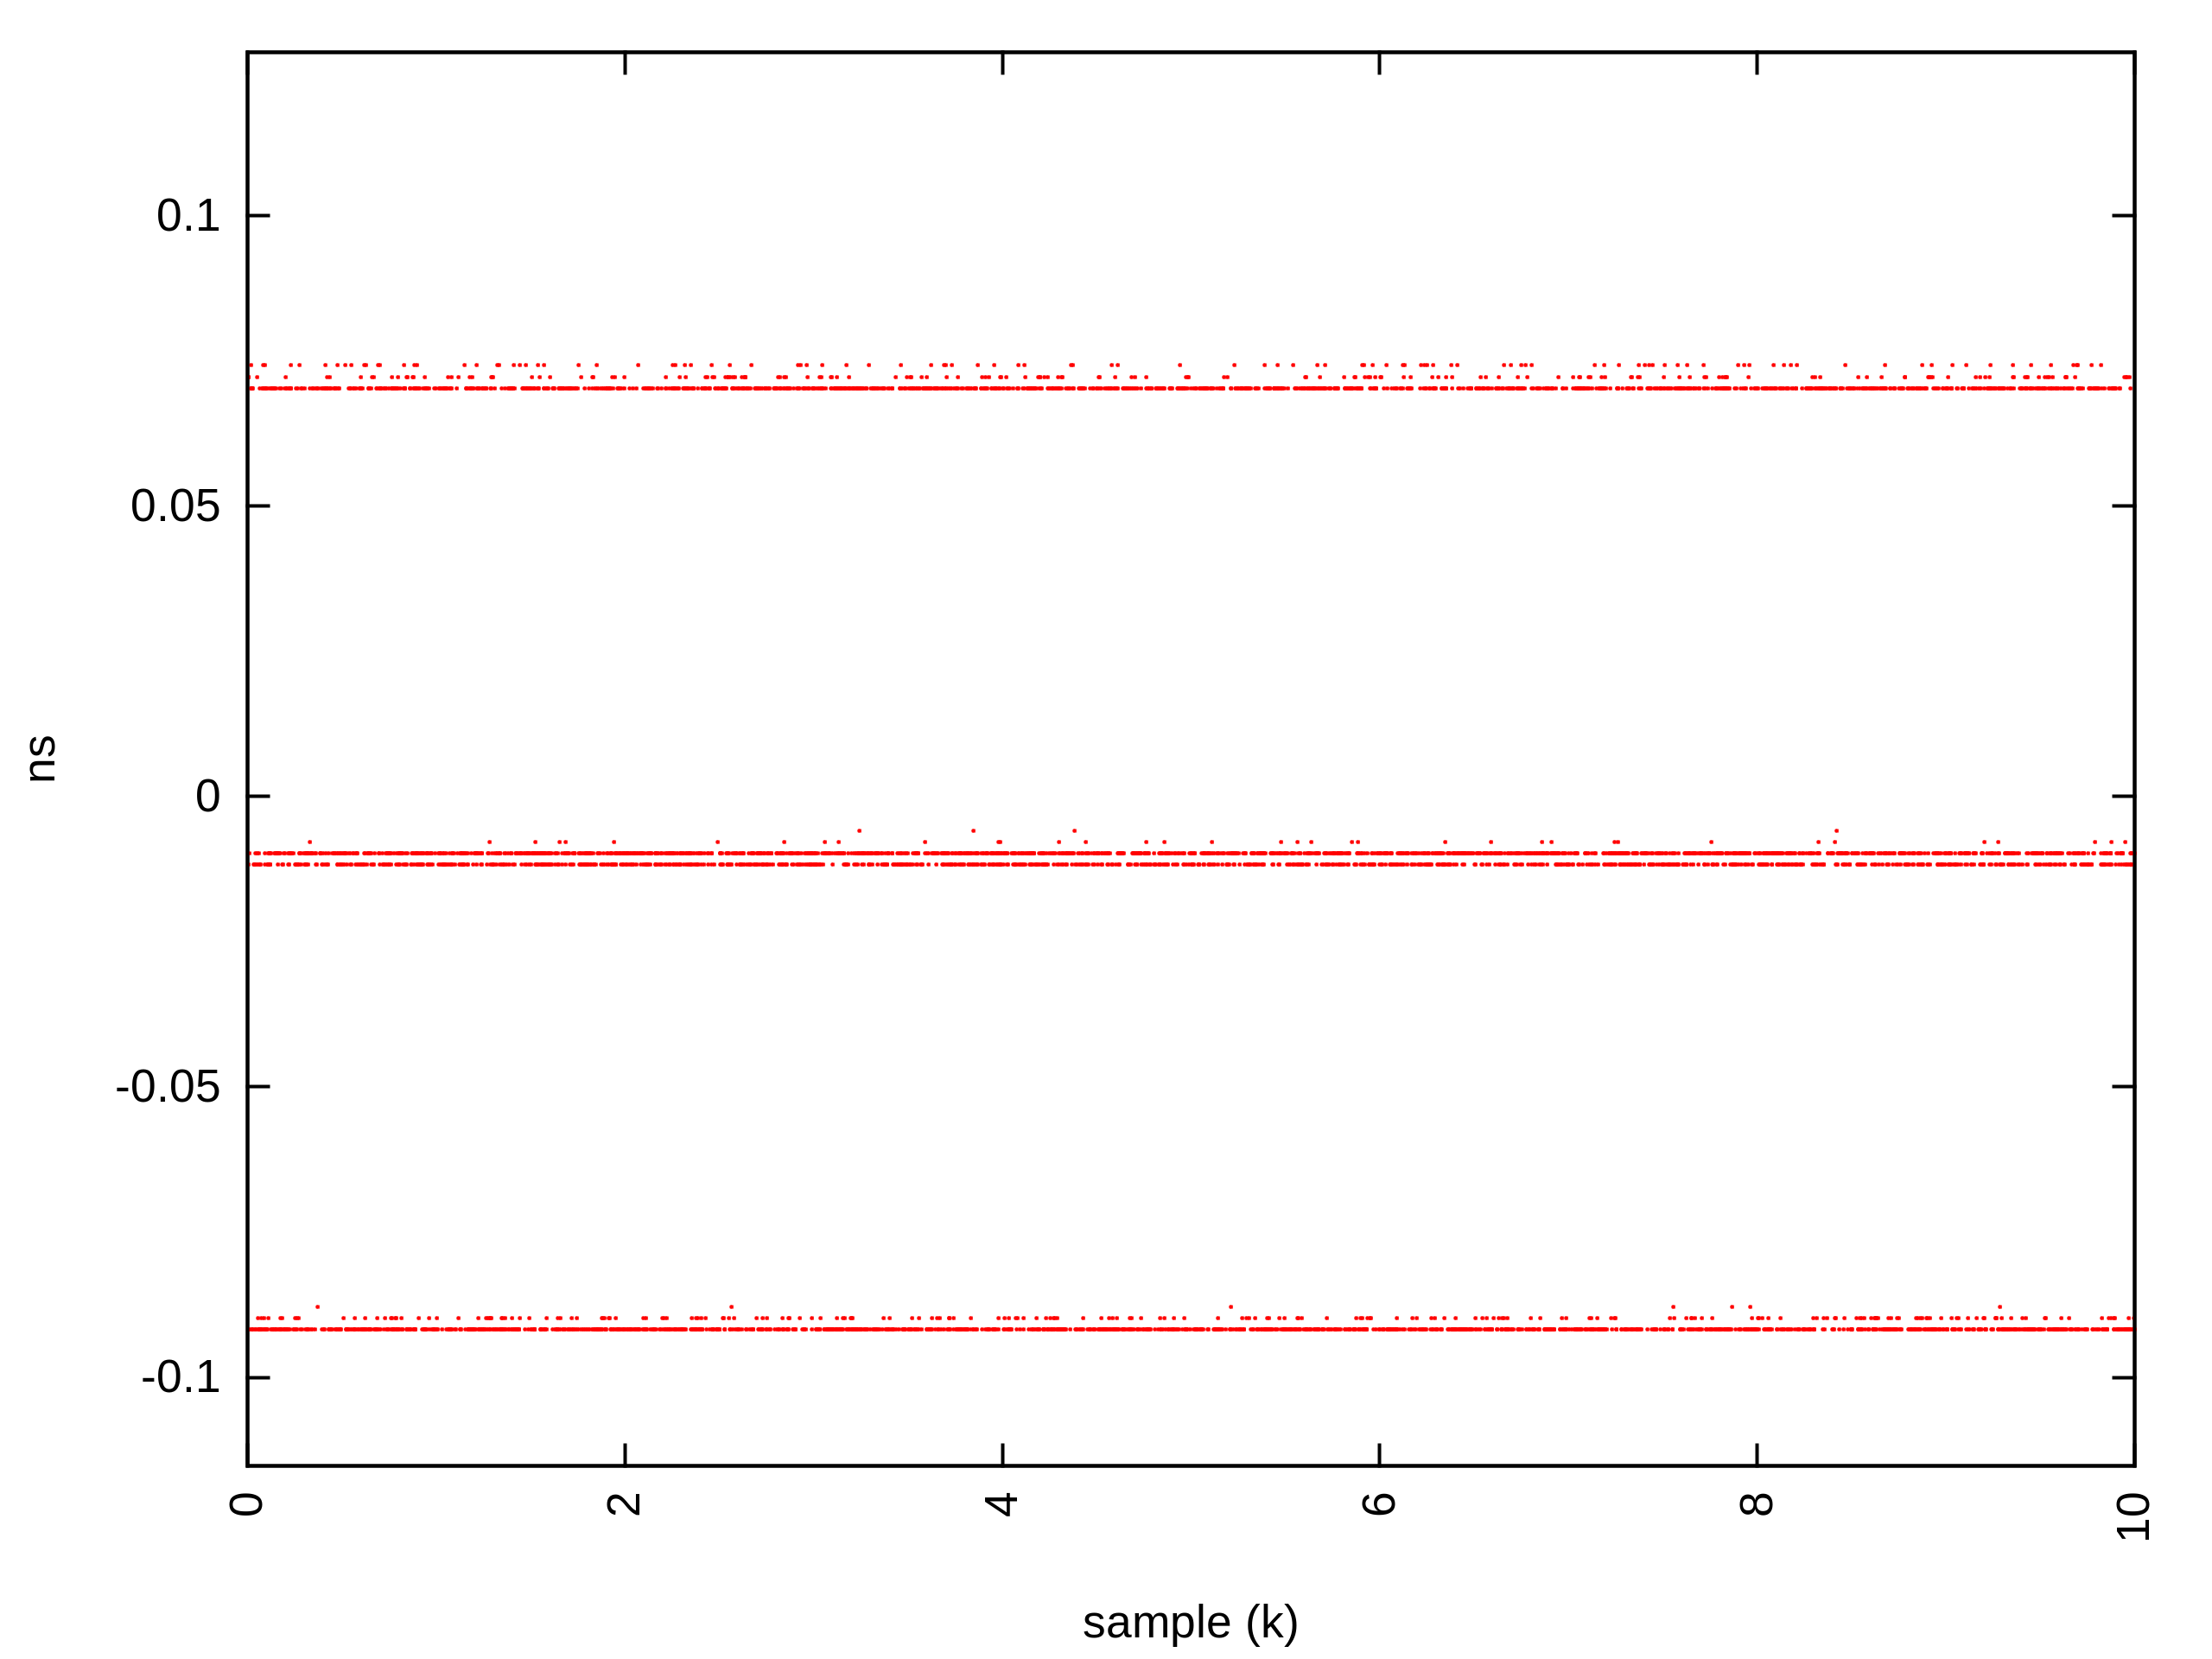
\includegraphics[width=0.7\textwidth]{img/test2_samples_relative_zoomxy.png}
  \caption{Test 2: Subset of acquired samples (relative timestamps)}
  \label{test2_relative_zoomy}
\end{figure}

The~Figure~\ref{test2_absolute} with absolute timestamps does not look like
an angled single line, similar to the~Figure~\ref{test1_absolute} with
absolute timestamps of the \textit{Test~1}. In the~Figure~\ref{test2_absolute}
samples draw many parallel horizontal lines. From the observation that samples
are visible as horizontal lines can be concluded that there is no drift between
clocks used on the pulse generator (Fine Delay) and the acquisition board (TDC).
Both used White Rabbit as the time reference.
It is believed that samples are spread into many parallel lines,
because of a precision limitation and a quantization effect of the timestamping
chip used on the TDC.
For an ideal chip, only one line would be present.

As seen on Figures~\ref{test2_absolute} and~\ref{test2_relative}, when
the White Rabbit is used, the comparison of relative and absolute timestamps
is not needed as both figures show similarities and no time drift is observed.

For figures with presented relative timestamps there is no visible difference
between results of \textit{Test~1} (Figure~\ref{test1_relative}) and
\textit{Test~2} (Figure~\ref{test2_relative}).

\FloatBarrier

\begin{figure}[ht!]
  \centering
  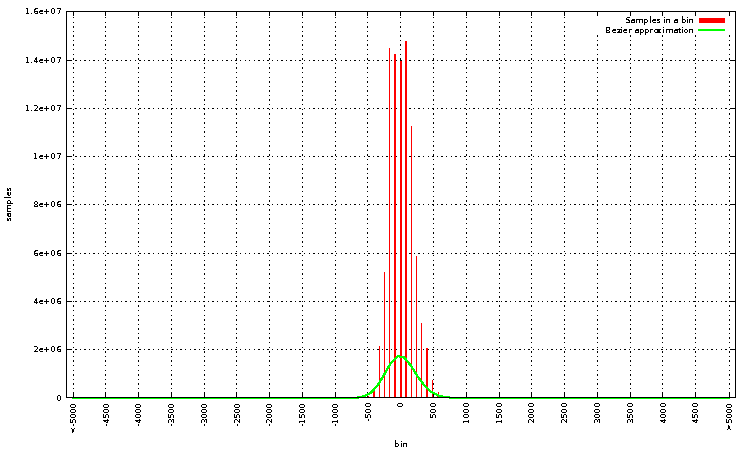
\includegraphics[width=0.80\textwidth]{img/test2_histogram.pdf}
  \caption{Test 2: Histogram of acquired samples (relative timestamps)}
  \label{test2_histogram}
\end{figure}

The same relative samples as above are
presented in the form of histogram in the~Figure~\ref{test2_histogram}.
Like in \textit{Test~1}, The histogram is divided into 1000 bins.
Each bin spans over 10 ps.
Two additional bins were added to keep all values greater and smaller than
5000ps.

As a consequence of the distribution of samples shown in
the~Figure~\ref{test2_relative}, there are many empty bins between filled bins
(like gaps between lines in the mentioned figure).
To overcome quantization effect and to give better overview
the Bezier approximation has been added to the histogram figure.

\begin{figure}[ht!]
  \centering
  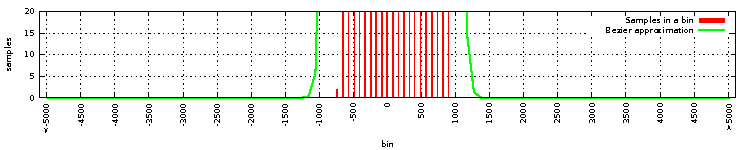
\includegraphics[width=1\textwidth]{img/test2_histogram_zoomy.pdf}
  \caption{Test 2: Histogram of acquired samples (relative timestamps)}
  \label{test2_histogram_zoomy}
\end{figure}

Figure~\ref{test2_histogram_zoomy} shows the zoom in on the Y axis of
the histogram presented in the~Figure~\ref{test2_histogram}.
This shows that all bins outside the center part of the figure are empty.
Similar to the \textit{Test~1} histogram (Figure~\ref{test2_histogram_zoomy}),
the Bezier curve may suggest that
there are samples outside the range -750ps to 1000ps, but all these bins are
empty.
This effect is due to the way how a Bezier curve is calculated.


\begin{figure}[ht!]
  \centering
  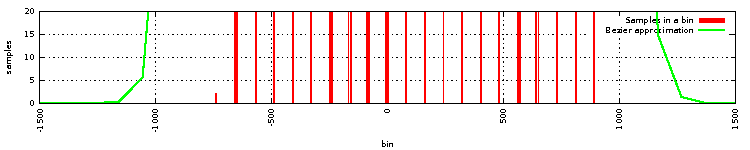
\includegraphics[width=1\textwidth]{img/test2_histogram_zoomx.pdf}
  \caption{Test 2: Histogram of acquired samples (relative timestamps),
           zoom in of the bottom center of the histogram
           (figure~\ref{test2_histogram})}
  \label{test2_histogram_zoomx}
\end{figure}
\FloatBarrier

Figure~\ref{test2_histogram_zoomx} shows the zoom in of the bottom center part
of the histogram presented in the~Figure~\ref{test2_histogram}.
It gives a better view about the presence of samples in bins that are close to
the center of the histogram.


\begin{table}[!htb]
  \centering
  \footnotesize
  \begin{tabular}{|r|r|r|r|r|r|r|}
    \hline {\bf Run} & {\bf Data Volume} & {\bf Mean (ps)} & {\bf Sigma (ps)} & {\bf Min (ps)} & {\bf Max (ps)} & {\bf Range (ps)}  \\
    \hline
    1                & 22.5M             &          0.000  &  165.093         &  -740.234      &   884.766      &     1625.000        \\
    2                & 30M               &          0.000  &  167.202         & -4466.800      &  4283.200      &     8750.000        \\
    **2              & 30M               &          0.000  &  167.198         &  -660.156      &   884.766      &     1544.922        \\
    3                & 100M              &          0.000  &  167.147         &  -740.234      &   884.766      &     1625.000        \\
    4                & 10M               &          0.000  &  149.314         &  -660.156      &   882.812      &     1542.969 \\

    \hline
  \end{tabular}
  \caption{Summary of \textit{Test~2} runs}
  \label{table_test2_summary}
\end{table}

In the run 2 there were two relative samples that have significantly differed
from other values.
It is suspected that this is the same bug as observed in the report
``TDC mezzanine board, Performance testing''
by E. Gousiou~\cite{tdc_perf_test}.
According to the bug, it might happen that the timestamping chip (ACAM) returns
the wrong timestamp with the offset about 4ns.
The table~\ref{table_test2_summary}
includes the calculations for the same run (marked with asterisk),
but without suspected timestamps. The Table~\ref{table_test2_samples_excluded}
includes the details about the excluded values.

The mean value of samples gathered in each run is very close to 0.
This proves that the time drift (thanks to White Rabbit) between
the pulse generator and the acquisition board is very small.

Other values like Sigma, Minimum, Maximum and Range are very similar to
the values included in the similar table for \textit{Test~1}
(Table~\ref{table_test1_summary}).

\begin{table}[!htb]
  \centering
  \footnotesize
  \begin{tabular}{|r|r|}
    \hline {\bf sample \#} & {\bf Delta (ps)} \\
    \hline
    25328569 & -4466.79687500 \\
    25328570 &  4283.20312500 \\
    \hline
  \end{tabular}
  \caption{Samples excluded from the run 2 of \textit{Test~2}}
  \label{table_test2_samples_excluded}
\end{table}

\FloatBarrier

To gather all data in the described test, the following python command has been
used:
\begin{lstlisting}
$ python -d -m pytest --usr-acq-count=100000000 --usr-acq-period-ns=1000000 \
  test_fmctdc_acquisition.py::TestFmctdcAcquisition::test_acq_timestamp_multiple_hist \
  --tdc-id-ch 0x17:1 --fd-id-ch 0x1a:1 --histogram-file test2_hist --bin-min-ps -5000 \
  --bin-max-ps 5000 --bins-num 1000 --samples-file test2 --tdc-wr-on
\end{lstlisting}

\FloatBarrier

\subsection{Test 3}
\label{test3}
Test summary:
\begin{center}
  \begin{tabular}{|l|l|}
    \hline {\bf Test parameter} & {\bf Value} \\
    \hline
    Pulse frequency                      & 1MHz and 2MHz \\
    Pulse width                          & 100ns \\
    Test duration                        & 5us \\
    Number of samples                    & 5K \\
    \hline
  \end{tabular}
\end{center}

This test is similar to the \textit{Test~2} (subsection~\ref{test2}) with
the exception of the much higher samples rate and much smaller number of
samples being acquired.
Both tests use White Rabbit as time reference for the pulse generator
and the acquisition board.
The minimal pulse width accepted by TDC is 96ns. In the preliminary tests
it has been observed that the maximum frequency of pulses that can be
acquired by the TDC is 5 MHz. Unfortunately, it has been observed that
with the current version of the TDC software and gateware the tested machine
can freeze if the samples' buffer is overwritten. To avoid the freeze
of a test machine the number of samples to be acquired is limited.

\begin{figure}[ht!]
  \centering
  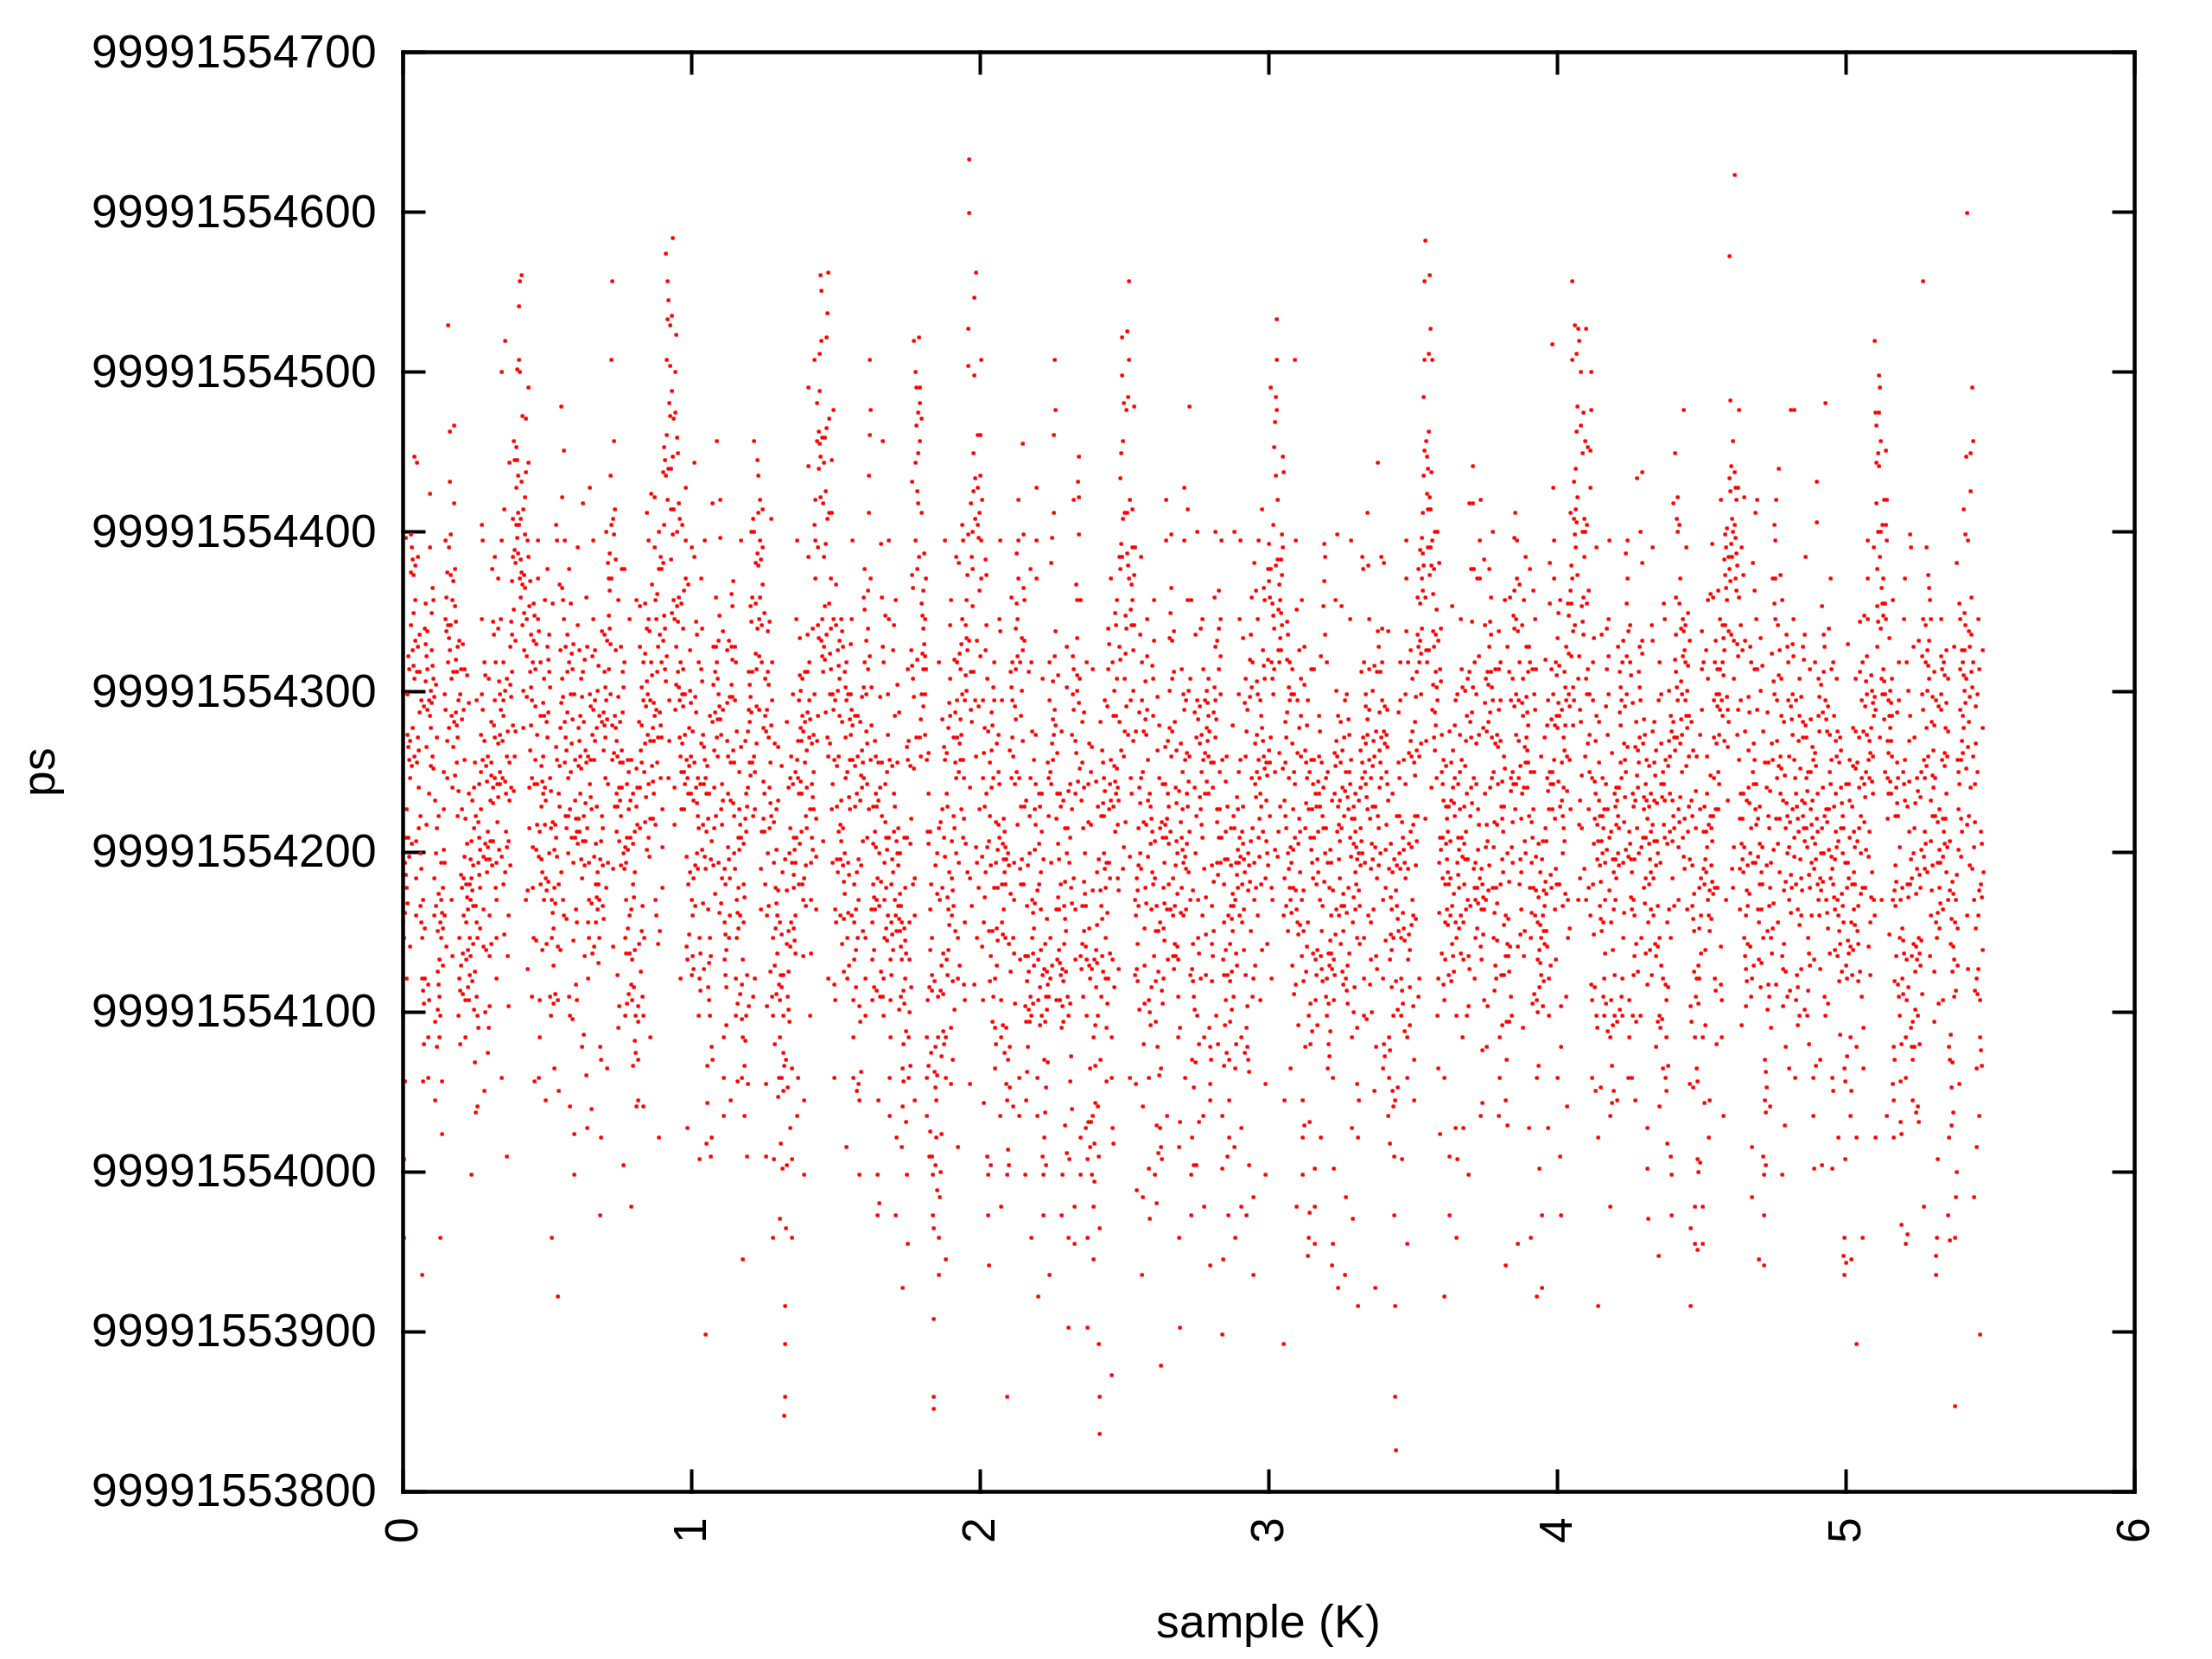
\includegraphics[width=0.80\textwidth]{img/test3_samples_absolute_1MHz.png}
  \caption{Test 3: Acquired samples (absolute timestamps), 1MHz sample rate}
  \label{test3_absolute_1MHz}
\end{figure}

\begin{figure}[ht!]
  \centering
  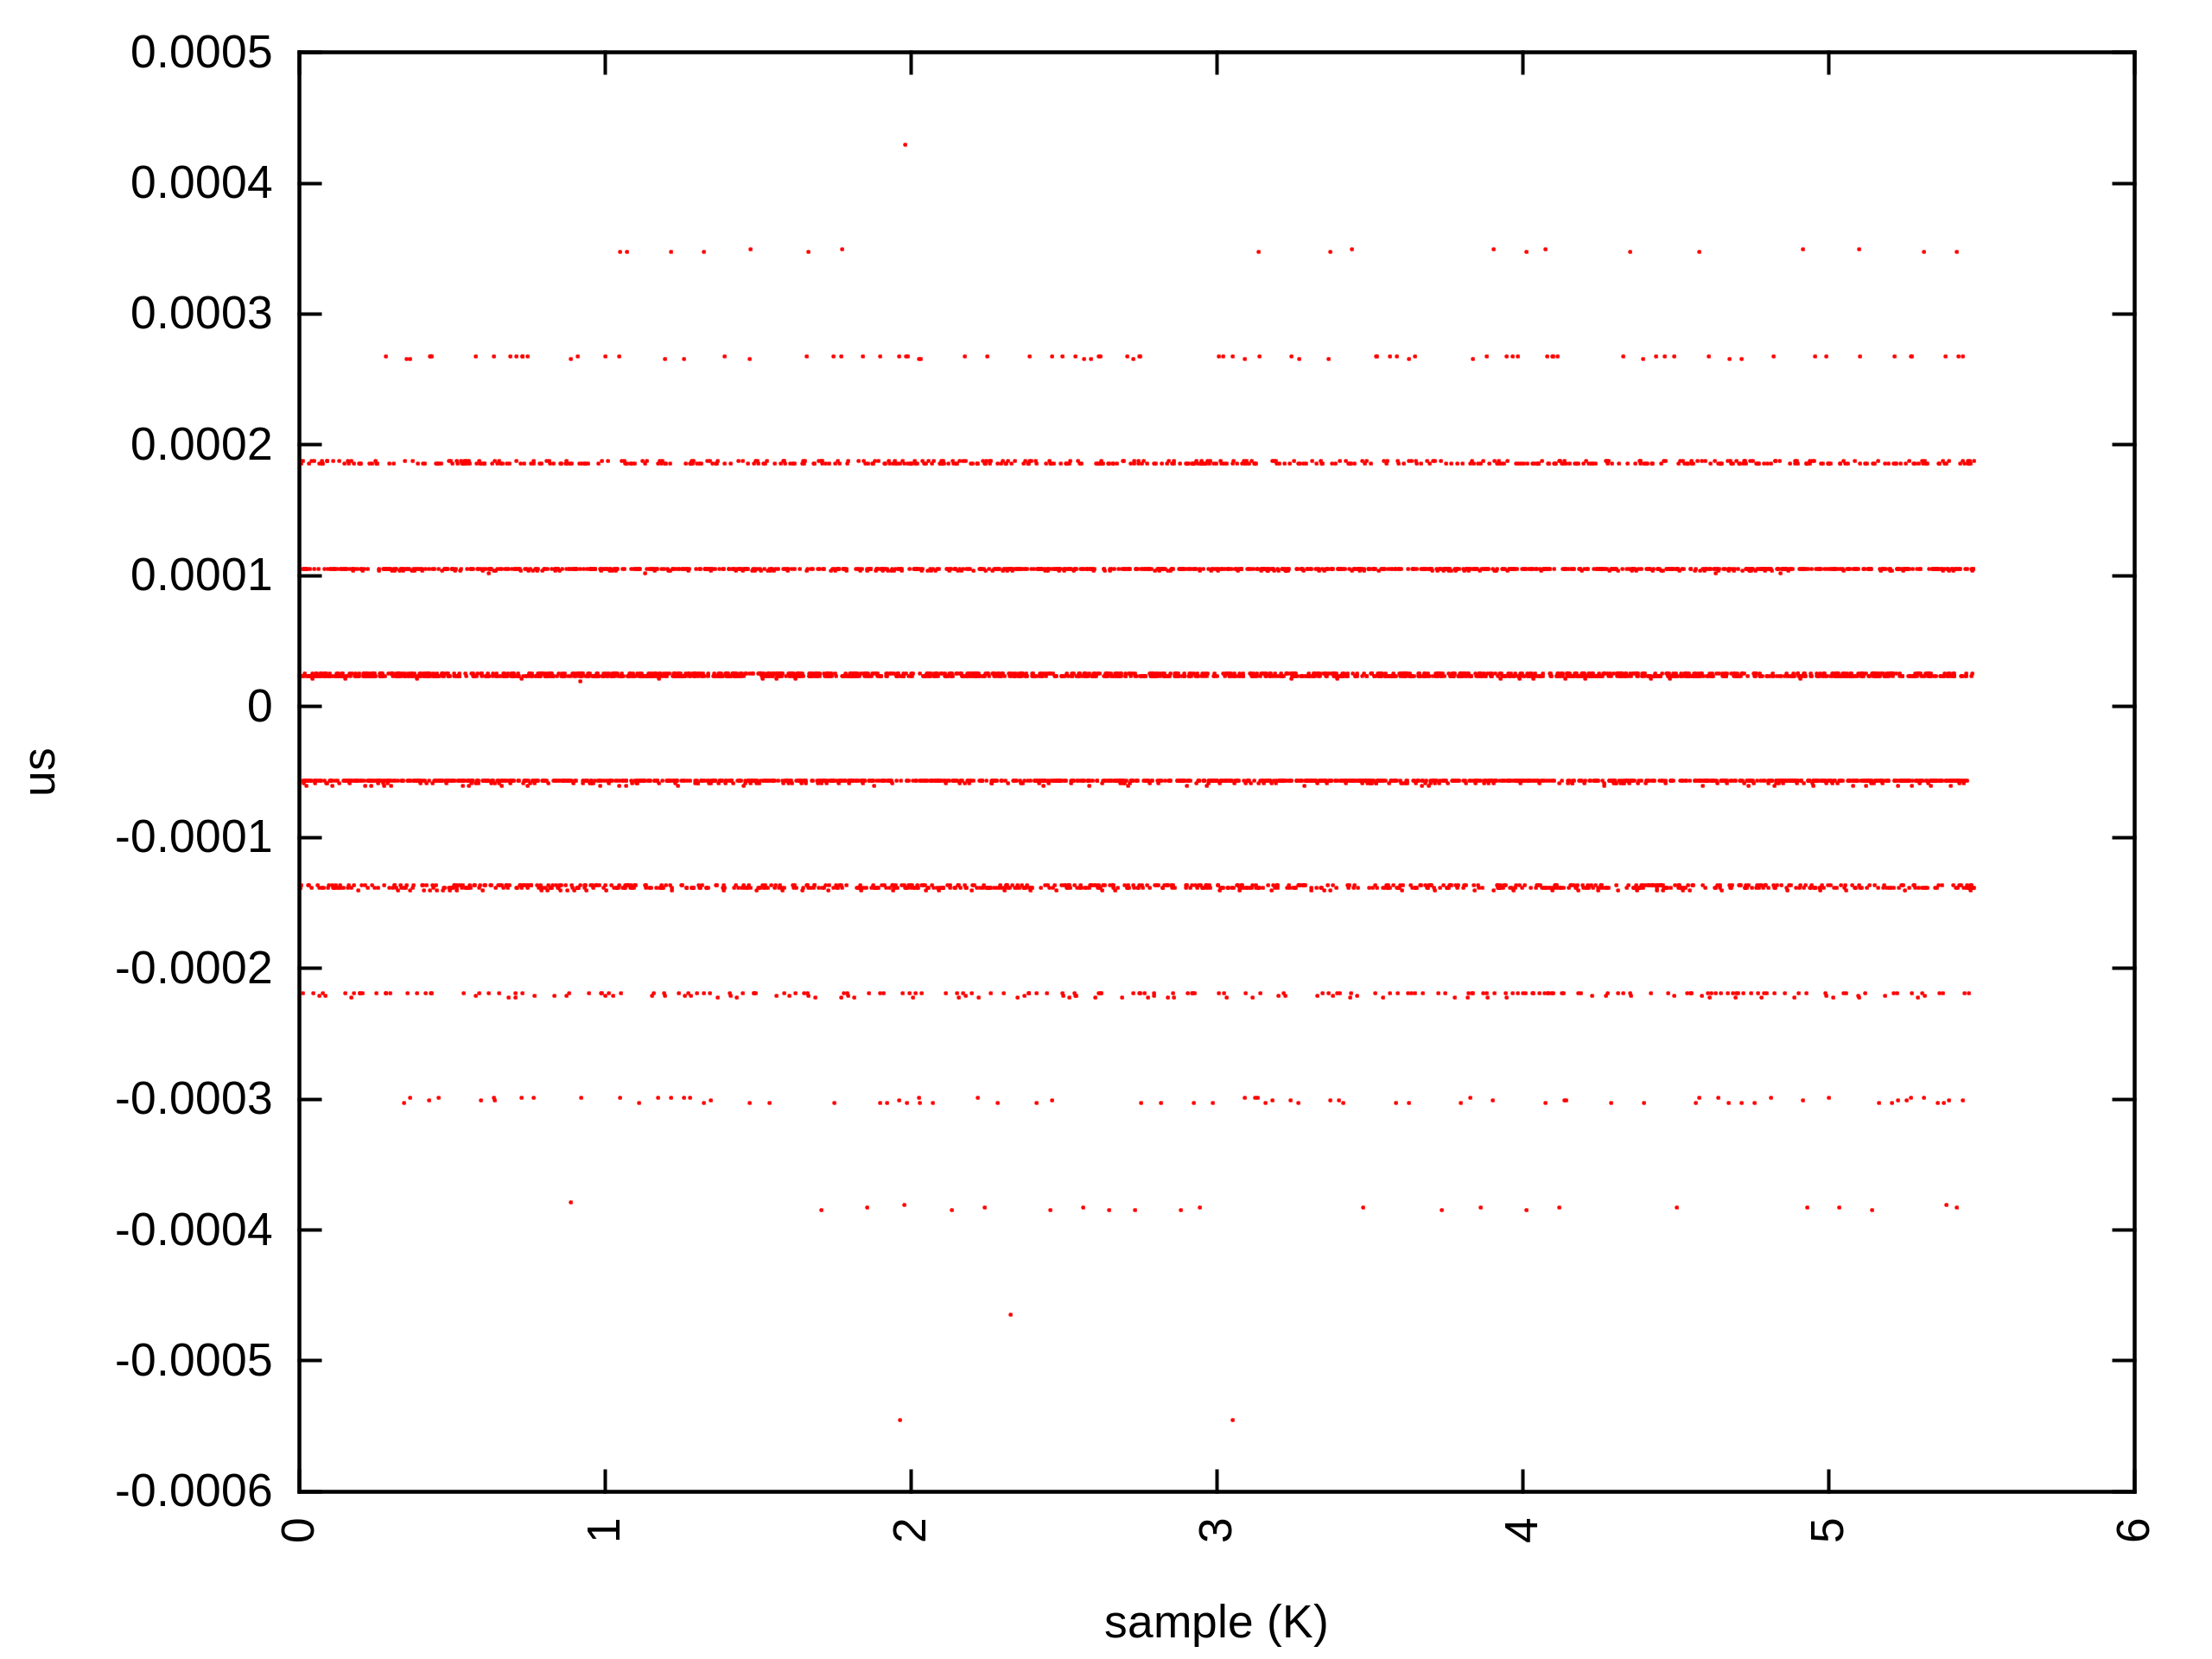
\includegraphics[width=0.8\textwidth]{img/test3_samples_relative_1MHz.png}
  \caption{Test 3: Acquired samples (relative timestamps), 1MHz sample rate}
  \label{test3_relative_1MHz}
\end{figure}

It was observed that when the pulse rate of a generated samples is 1MHz,
the TDC was able to acquire about 6k samples in one burst.
The~Figure~\ref{test3_absolute_1MHz} presents absolute timestamps,
Figure~\ref{test3_relative_1MHz} presents relative timestamps.
The distribution of samples is similar to the results observed in
\textit{Test~2} (Figure~\ref{test2_absolute} and~Figure~\ref{test2_relative}).

\FloatBarrier
\begin{figure}[ht!]
  \centering
  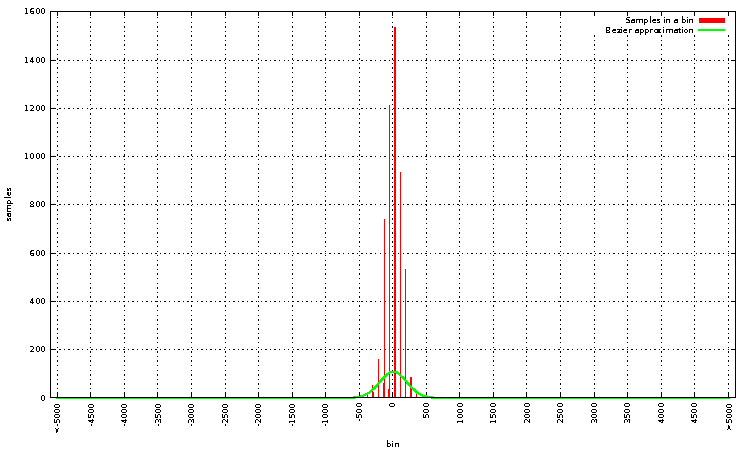
\includegraphics[width=0.80\textwidth]{img/test3_histogram_1MHz.pdf}
  \caption{Test 3: Histogram of acquired samples (relative timestamps),
           1MHz sample rate}
  \label{test3_histogram_1MHz}
\end{figure}

\begin{figure}[ht!]
  \centering
  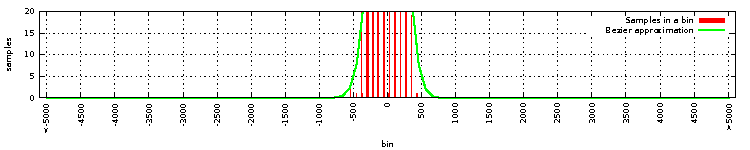
\includegraphics[width=1\textwidth]{img/test3_histogram_zoomy_1MHz.pdf}
  \caption{Test 3: Histogram of acquired samples (relative timestamps),
           1MHz sample rate, zoom in on the Y axis of the histogram
           (Figure~\ref{test3_histogram_1MHz})}
  \label{test3_histogram_zoomy_1MHz}
\end{figure}

Figure~\ref{test3_histogram_1MHz} presents the histogram of acquired relative
timestamps. Zoom in on the Y axis is presented in
the~Figure~\ref{test3_histogram_zoomy_1MHz}.
Zoom in on the center bottom part is presented in
the~Figure~\ref{test3_histogram_zoomx_1MHz}.
It shows that all bins outside the center part of the figure are empty.
Also for this figure, the distribution of samples is similar to the results
observed in
\textit{Test~2} (Figure~\ref{test2_absolute} and~Figure~\ref{test2_relative}).

\begin{figure}[ht!]
  \centering
  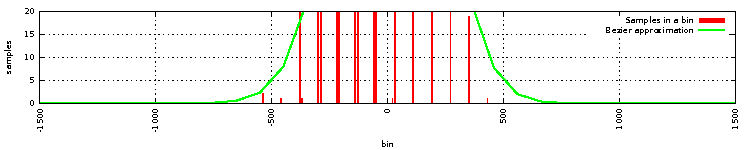
\includegraphics[width=1\textwidth]{img/test3_histogram_zoomx_1MHz.pdf}
  \caption{Test 3: Histogram of acquired samples (relative timestamps),
           1MHz sample rate, zoom in of the bottom center part of the histogram
           (Figure~\ref{test3_histogram_1MHz})}
  \label{test3_histogram_zoomx_1MHz}
\end{figure}

\FloatBarrier

\begin{figure}[ht!]
  \centering
  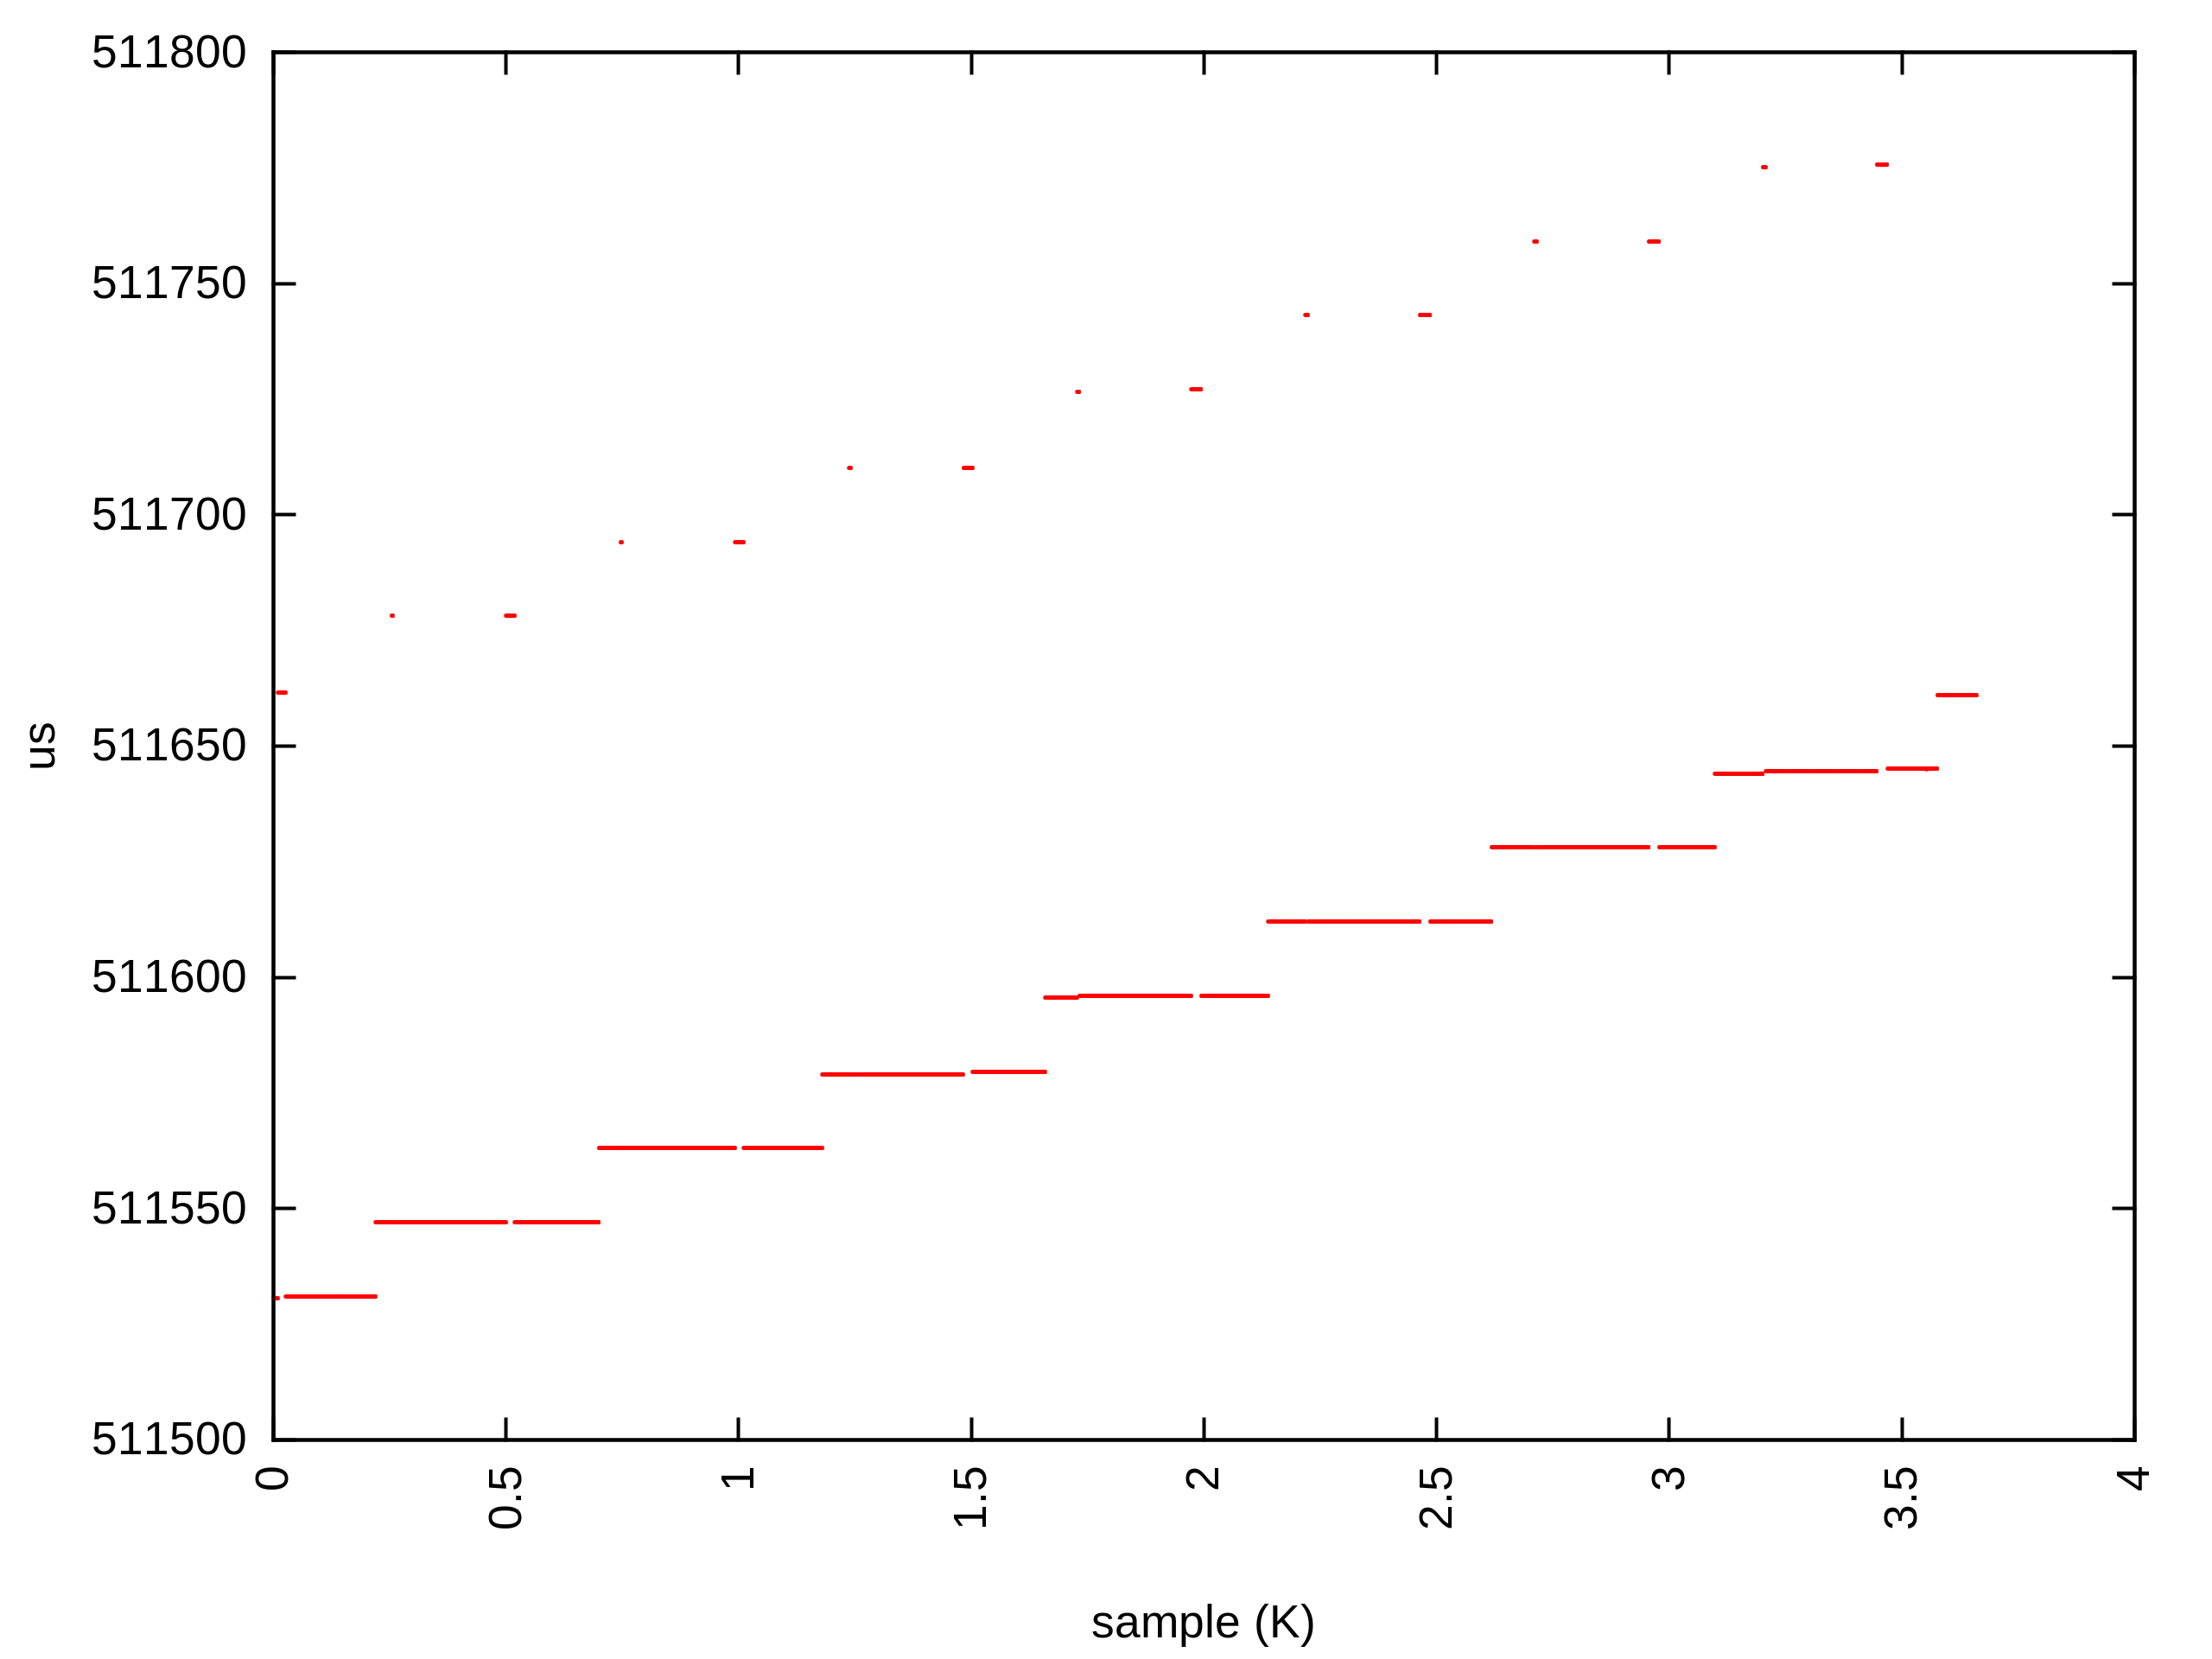
\includegraphics[width=0.80\textwidth]{img/test3_samples_absolute_2MHz.png}
  \caption{Test 3: Acquired samples (absolute timestamps), 2MHz sample rate}
  \label{test3_absolute_2MHz}
\end{figure}

\begin{figure}[ht!]
  \centering
  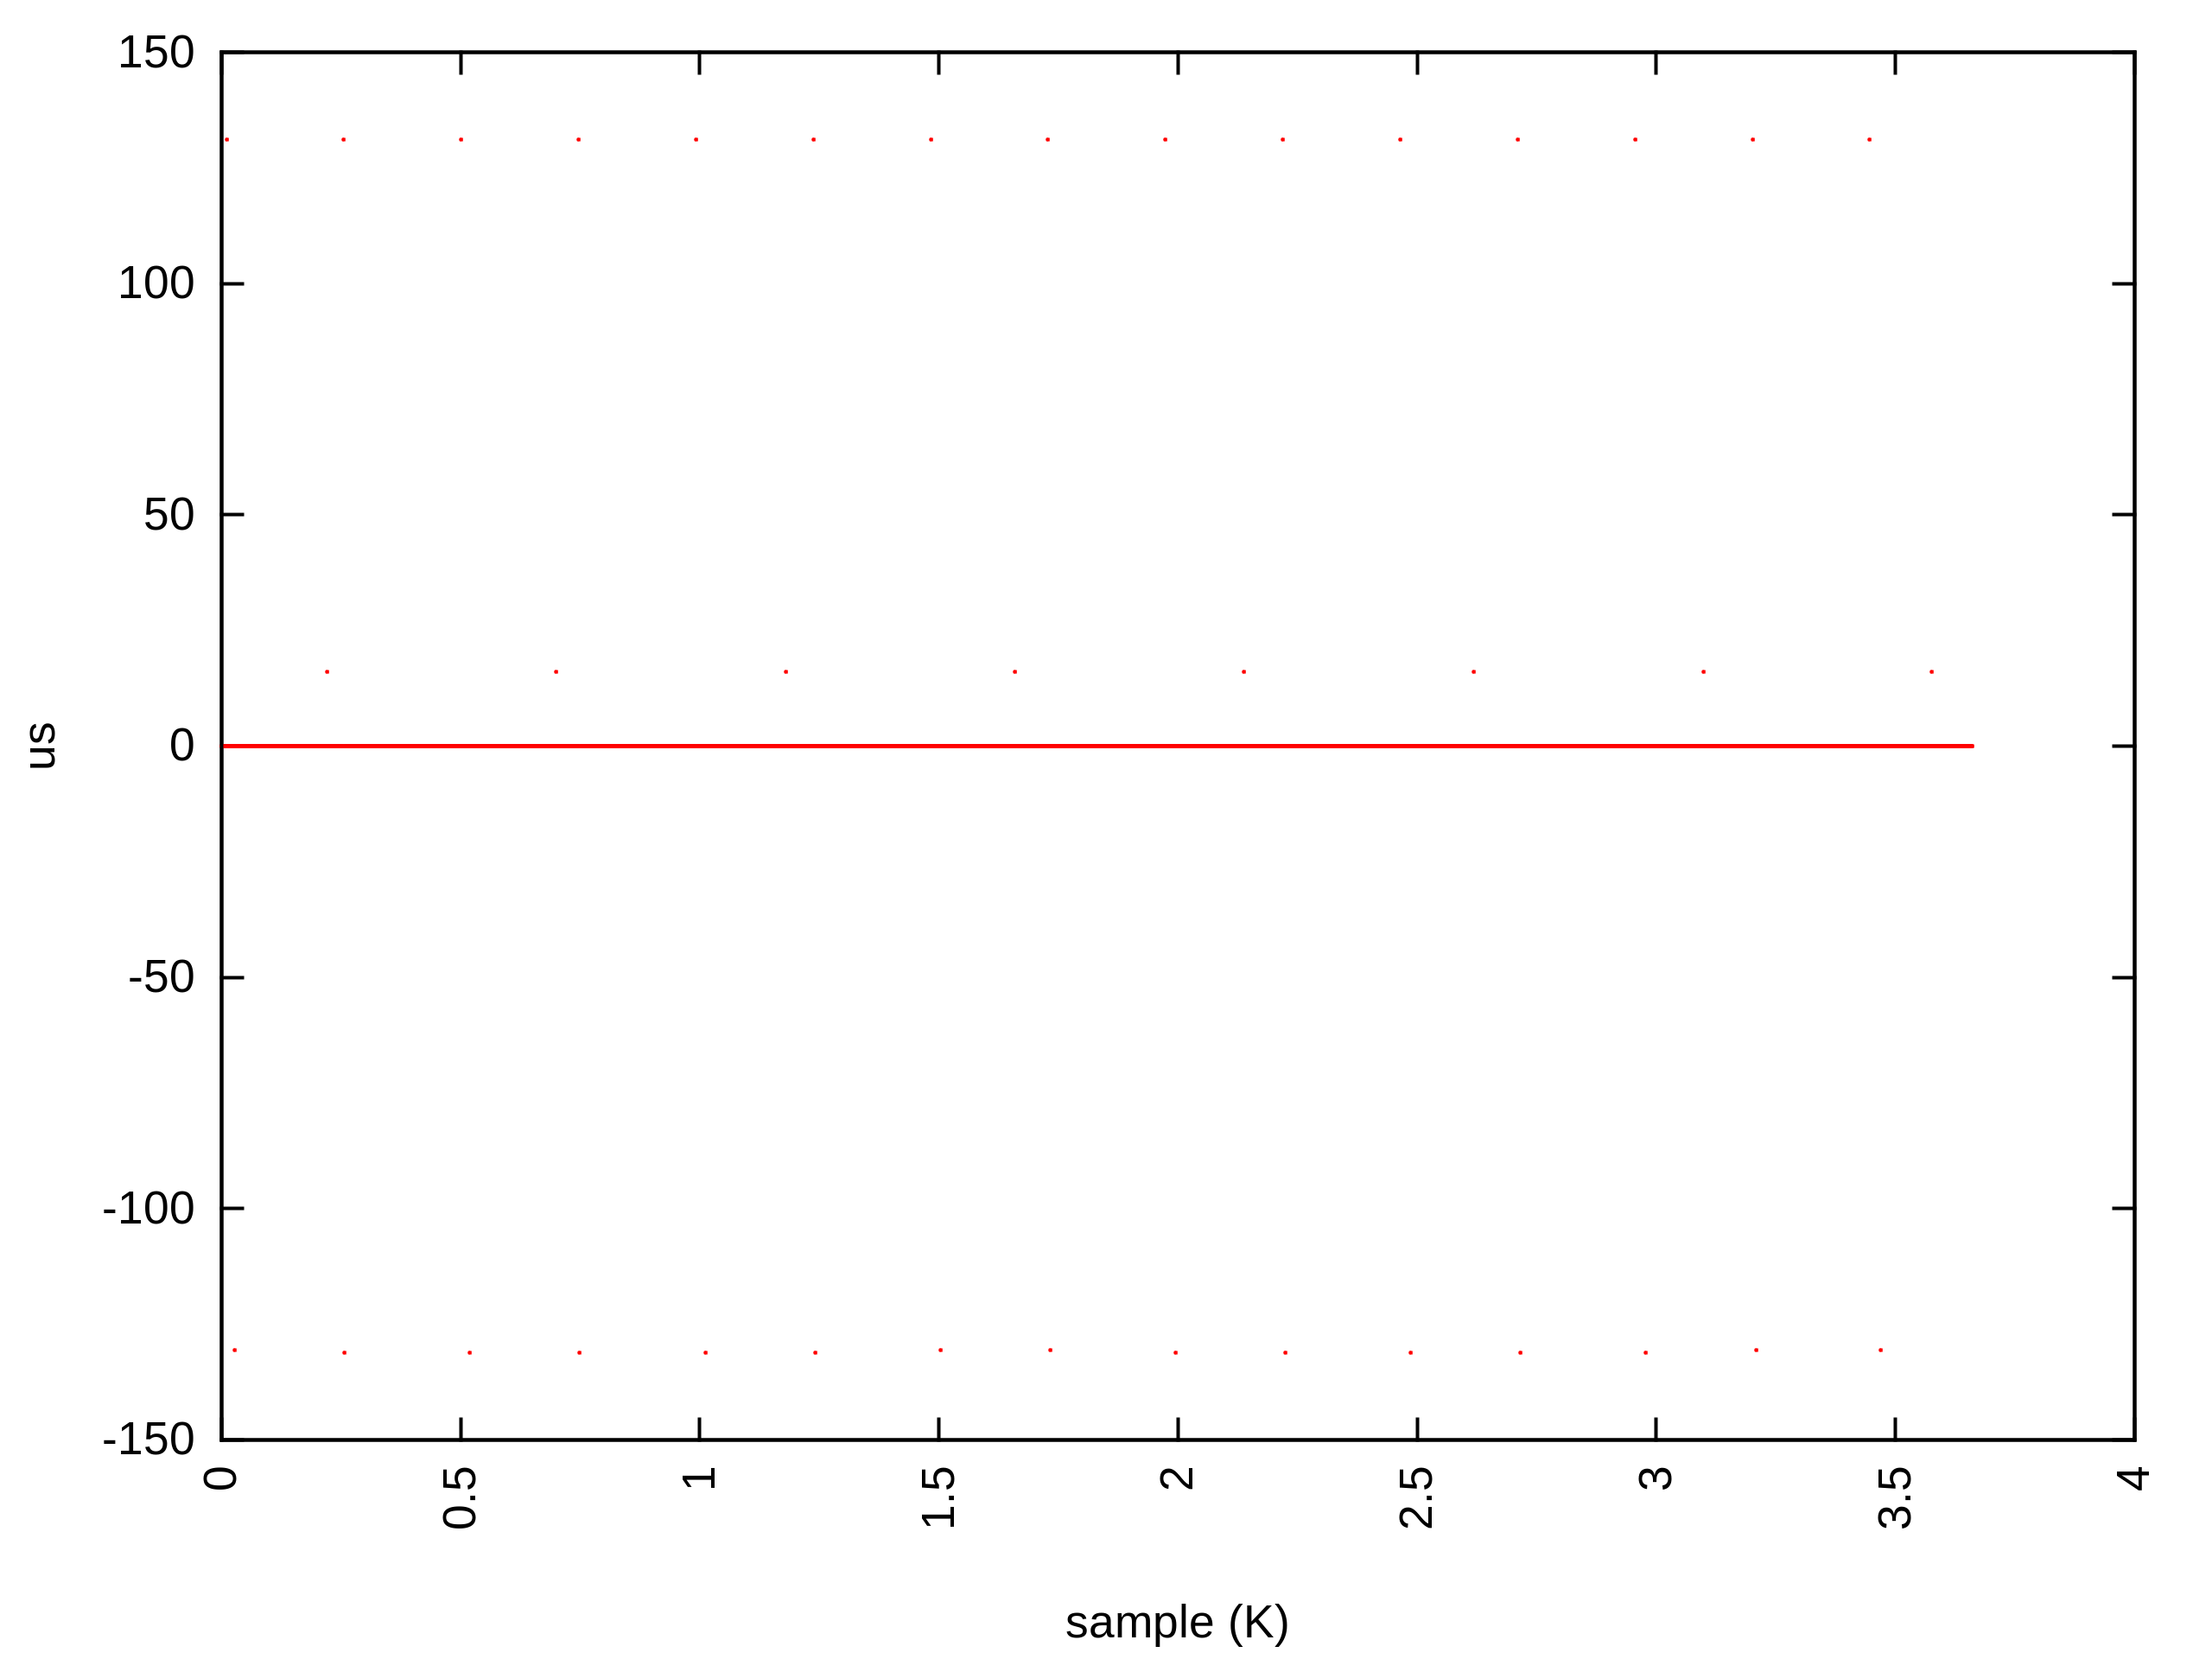
\includegraphics[width=0.8\textwidth]{img/test3_samples_relative_2MHz.png}
  \caption{Test 3: Acquired samples (relative timestamps), 2MHz sample rate}
  \label{test3_relative_2MHz}
\end{figure}

The same test has been run once more, this time with 2MHz sample rate.
Number of samples were lost periodically, which can be observed as
jumps in~Figure~\ref{test3_absolute_2MHz}.

It is worth to notice, that sequence IDs reported to the test program
were consecutive for all samples.
The only way to conclude that samples are missing is to analyze
the acquired timestamps.

Looking at the~Figure~\ref{test3_relative_2MHz} it is also easy to spot
the jumps in timestamps.
For relative timestamps such jumps are presented as single non-symmetrical
data points just above line at 0us.

\FloatBarrier


\begin{figure}[ht!]
  \centering
  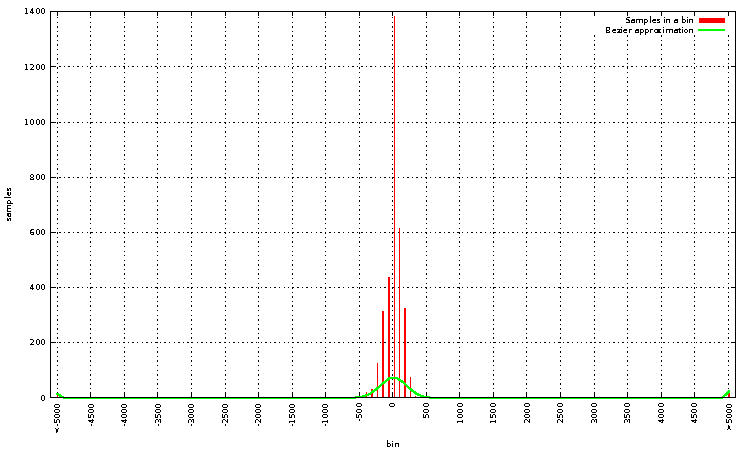
\includegraphics[width=0.80\textwidth]{img/test3_histogram_2MHz.pdf}
  \caption{Test 3: Histogram of acquired samples (relative timestamps),
           2MHz sample rate}
  \label{test3_histogram_2MHz}
\end{figure}

\begin{figure}[ht!]
  \centering
  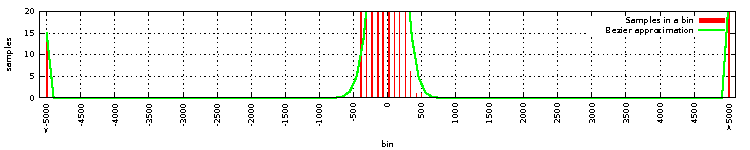
\includegraphics[width=1\textwidth]{img/test3_histogram_zoomy_2MHz.pdf}
  \caption{Test 3: Histogram of acquired samples (relative timestamps),
           2MHz sample rate, zoom in on the Y axis of the histogram
           (Figure~\ref{test3_histogram_2MHz})}
  \label{test3_histogram_zoomy_2MHz}
\end{figure}

\begin{figure}[ht!]
  \centering
  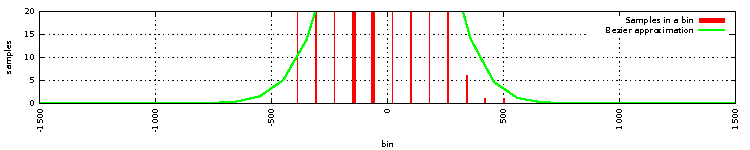
\includegraphics[width=1\textwidth]{img/test3_histogram_zoomx_2MHz.pdf}
  \caption{Test 3: Histogram of acquired samples (relative timestamps),
           2MHz sample rate, zoom in of the bottom center part of the histogram
           (Figure~\ref{test3_histogram_2MHz})}
  \label{test3_histogram_zoomx_2MHz}
\end{figure}

Unlike other histograms, in this case there are samples in the bins on
the sides of the histogram (samples below and above 5ns),
visible better in the zoom in on the Y axis
(Figure~\ref{test3_histogram_zoomy_2MHz}).

The center part of the histogram (zoom in can be seen in
the~Figure~\ref{test3_histogram_zoomx_2MHz}) looks very similar to the run with
1MHz sample rate (Figure~\ref{test3_histogram_1MHz}).

All other bins i.e. between outside center part of the histogram and edges are
empty.
This demonstrate that even if some samples were dropped, the rest of acquired
samples are in line with observations done in other tests.


\FloatBarrier

\begin{table}[!htb]
  \centering
  \scriptsize
  \begin{tabular}{|r|r|r|r|r|r|r|r|}
    \hline
    {\bf Run} & {\bf \begin{tabular}{@{}c@{}}Sample \\ Rate\end{tabular}} & {\bf \begin{tabular}{@{}c@{}}Data \\ Volume\end{tabular}} & {\bf Mean (ps)} & {\bf Sigma (ps)} & {\bf Min (ps)} & {\bf Max (ps)} & {\bf Range (ps)}  \\
    \hline
    1         &  1MHz             & 5K             &          0.010 & 120.476 & -544.922 & 429.688 & 974.609 \\
    2         &  1MHz             & 5K             &          0.004 & 121.566 & -464.844 & 429.688 & 894.531 \\
    3         &  2MHz             & 5K             &          35645.958 & 11881057.859 & -131072150.391 & 131072255.859 & 262144406.250 \\
    4         &  2MHz             & 5K             &          34962.034 & 11270298.808 & -131072148.438 & 131072093.750 & 262144242.188 \\
    \hline
  \end{tabular}
  \caption{Summary of \textit{Test~3} runs}
  \label{table_test3_summary}
\end{table}

Values in the rows representing runs with 1MHz sample rate (run~1 and~2) in
the Table~\ref{table_test3_summary} are very similar
to values presented in similar tables (like~\ref{table_test2_summary})
in other sections.
On the other hand, values in rows representing runs with 2MHz sample rate
(run~3 and~4) are significantly different.

To gather data for 1MHz sample rate in the described test,
the following command has been used:
\begin{lstlisting}
$ python -d -m pytest --usr-acq-count=5000 --usr-acq-period-ns=1000 \
  test_fmctdc_acquisition.py::TestFmctdcAcquisition::test_acq_timestamp_multiple_hist \
  --tdc-id-ch 0x18:0 --fd-id-ch 0x1a:1 --bin-min-ps -5000 --bin-max-ps 5000 \
  --bins-num 1000 --histogram-file=test3_hist --samples-file=test3_sample --tdc-wr-on
\end{lstlisting}

Very similar command used for 2MHz sample rate:
\begin{lstlisting}
$ python -d -m pytest --usr-acq-count=5000 --usr-acq-period-ns=500 \
  test_fmctdc_acquisition.py::TestFmctdcAcquisition::test_acq_timestamp_multiple_hist \
  --tdc-id-ch 0x18:0 --fd-id-ch 0x1a:1 --bin-min-ps -5000 --bin-max-ps 5000 \
  --bins-num 1000 --histogram-file=test3_hist --samples-file=test3_sample --tdc-wr-on
\end{lstlisting}

\FloatBarrier

\subsection{Test 4}
\label{test4}

Test summary:
\begin{center}
  \begin{tabular}{|l|l|}
    \hline {\bf Test parameter} & {\bf Value} \\
    \hline
    Pulse frequency                      & 250Hz \\
    Pulse width                          & 1000ns \\
    Test duration                        & 11hours \\
    Number of samples                    & 10M per channel \\
    Number of channels                   & 15 (5 per board) \\
    \hline
  \end{tabular}
\end{center}

In this test timestamps were acquired simultaneously from 15 (all available)
channels of three different TDCs. Due to the amount of the incoming data,
the pulse rate is less than in other tests covered in this report.


To make the histogram figure clearer the Figure~\ref{test4_histogram_5ch}
contains the histogram of the data acquired
only from 5 channels on the same board. Figure with all 15 channels
is included in the later part of this subsection
(Figure~\ref{test4_histogram_15ch}).
Similar to other tests, to overcome quantization effect and to give better
overview Bezier approximations were added to histogram figures.


\begin{figure}[ht!]
  \centering
  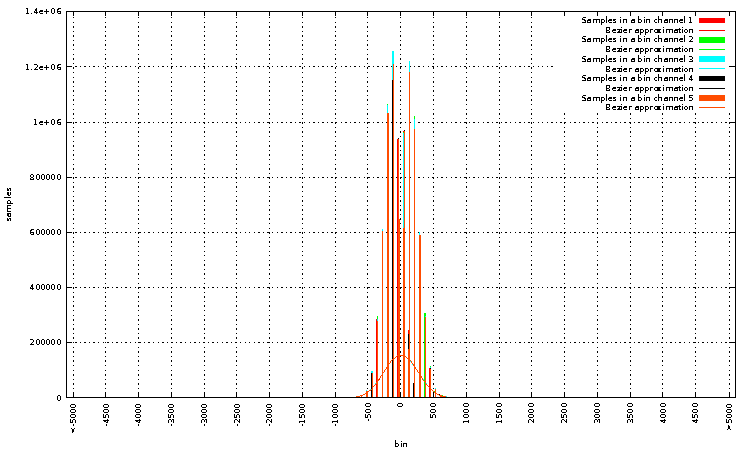
\includegraphics[width=0.80\textwidth]{img/test4_histogram_5ch.pdf}
  \caption{Test 4: Histogram of acquired samples from 5 channels}
  \label{test4_histogram_5ch}
\end{figure}

The zoom in of the~Figure~\ref{test4_histogram_5ch} is presented in
the~Figure~\ref{test4_histogram_5ch_zoomy} (Y axis) and
Figure~\ref{test4_histogram_5ch_zoomxy} (bottom center part).

As seen on zoomed histograms, number of samples in bins and Bezier
approximations of the data from different channels overlap with no significant
differences. Based on this it can be concluded that all channels behave in
the very similar way.


\begin{figure}[ht!]
  \centering
  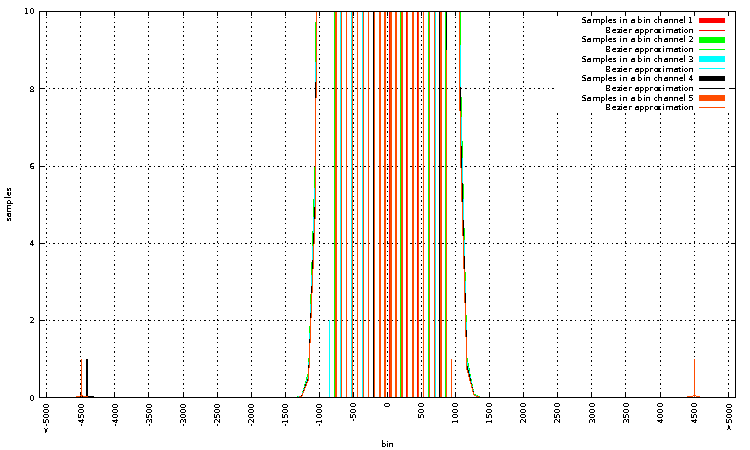
\includegraphics[width=0.80\textwidth]{img/test4_histogram_5ch_zoomy.pdf}
  \caption{Test 4: Histogram of acquired samples from 5 channels,
	  zoom in on the Y axis of the histogram
	  (Figure~\ref{test4_histogram_5ch})}
  \label{test4_histogram_5ch_zoomy}
\end{figure}

\begin{figure}[ht!]
  \centering
  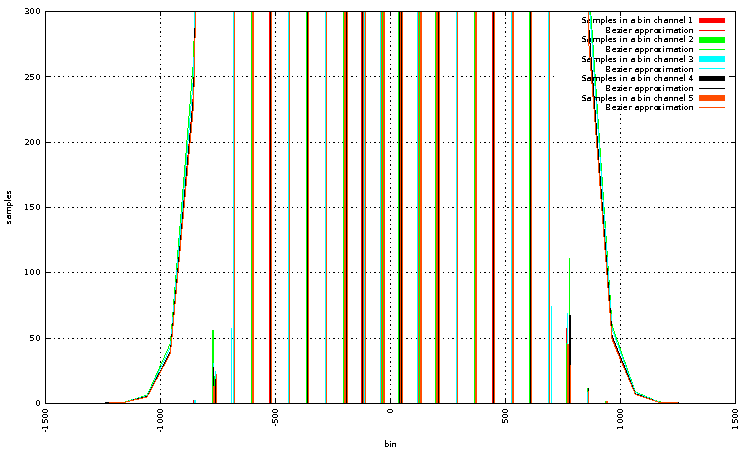
\includegraphics[width=0.80\textwidth]{img/test4_histogram_5ch_zoomxy.pdf}
  \caption{Test 4: Histogram of acquired samples from 5 channels, zoom
	   of the bottom center part of the histogram
	   (Figure~\ref{test4_histogram_5ch})}
  \label{test4_histogram_5ch_zoomxy}
\end{figure}

Please note that channels 1-4 are connected to the same input channel on
the ACAM chip, while the channel 5 is on another channel on ACAM chip.

\FloatBarrier

Figure~\ref{test4_histogram_15ch} contains the histogram of the full data
acquired in this test, 15 channels from three TDC boards.
This histogram also includes Bezier approximations for each channel.

The zoom in of the~Figure~\ref{test4_histogram_15ch} is presented in
the~Figure~\ref{test4_histogram_15ch_zoomy} (zoom in of the Y axis) and
Figure~\ref{test4_histogram_15ch_zoomxy} (zoom in on bottom center part).

As seen on the zoomed histograms, number of samples in bins and Bezier
approximations of the data from different channels overlap with no significant
differences. Based on this it can be concluded that all channels,
even on different boards, behave in the same way.


\begin{figure}[ht!]
  \centering
  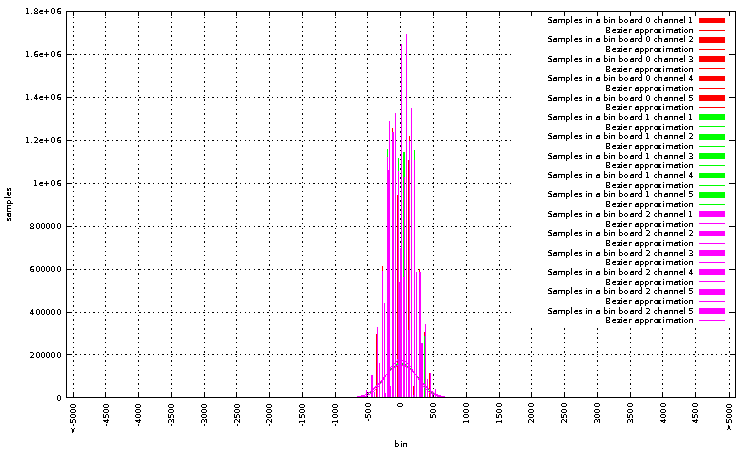
\includegraphics[width=0.80\textwidth]{img/test4_histogram_15ch.pdf}
  \caption{Test 4: Histogram of acquired samples from 15 channels (3 boards)}
  \label{test4_histogram_15ch}
\end{figure}

\begin{figure}[ht!]
  \centering
  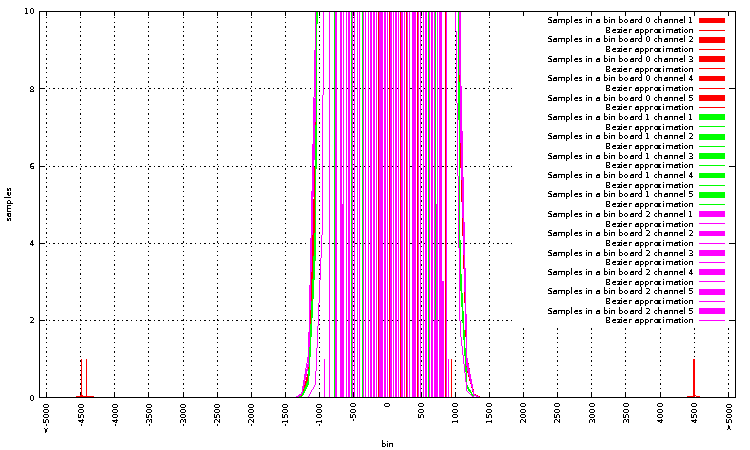
\includegraphics[width=0.80\textwidth]{img/test4_histogram_15ch_zoomy.pdf}

  \caption{Test 4: Histogram of acquired samples from 15 channels (3 boards),
	  zoom in on the Y axis of the histogram
	  (Figure~\ref{test4_histogram_15ch})}
  \label{test4_histogram_15ch_zoomy}
\end{figure}

\begin{figure}[ht!]
  \centering
  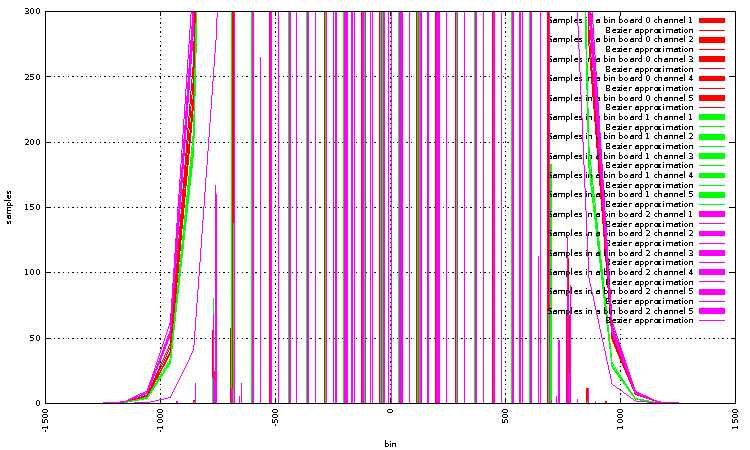
\includegraphics[width=0.80\textwidth]{img/test4_histogram_15ch_zoomxy.pdf}
  \caption{Test 4: Histogram of acquired samples from 5 channels (3 boards),
	  zoom in of the bottom center part of the histogram
	  (Figure~\ref{test4_histogram_15ch})}
  \label{test4_histogram_15ch_zoomxy}
\end{figure}

\FloatBarrier

Statistical summary of a single run of \textit{Test~4} is presented in
the~Table~\ref{table_test4_summary}.

\begin{table}[!htb]
% \begin{center}
\centering
\footnotesize
  \begin{tabular}{|c|c|r|r|r|r|r|}
    \hline {\bf Board} & {\bf Channel} & {\bf Mean (ps)} & {\bf Sigma (ps)} & {\bf Min (ps)} & {\bf Max (ps)} & {\bf Range (ps)}  \\
    \hline
    1 & 1 & 0.000 & 190.677 & -851.562 & 931.641 & 1783.203 \\
1 & 2 & 0.000 & 193.169 & -851.562 & 931.641 & 1783.203 \\
1 & 3 & 0.000 & 192.445 & -851.562 & 851.562 & 1703.125 \\
1 & 4 & 0.000 & 190.439 & -4414.062 & 4496.094 & 8910.156 \\
1 & 5 & 0.000 & 189.851 & -4496.094 & 4496.094 & 8992.188 \\
2 & 1 & 0.000 & 183.220 & -771.484 & 771.484 & 1542.969 \\
2 & 2 & 0.000 & 184.114 & -853.516 & 771.484 & 1625.000 \\
2 & 3 & 0.000 & 183.969 & -851.562 & 851.562 & 1703.125 \\
2 & 4 & 0.000 & 182.936 & -851.562 & 771.484 & 1623.047 \\
2 & 5 & 0.000 & 182.632 & -771.484 & 771.484 & 1542.969 \\
3 & 1 & 0.000 & 193.824 & -851.562 & 851.562 & 1703.125 \\
3 & 2 & 0.000 & 197.143 & -851.562 & 851.562 & 1703.125 \\
3 & 3 & 0.000 & 196.128 & -851.562 & 851.562 & 1703.125 \\
3 & 4 & 0.000 & 196.127 & -931.641 & 851.562 & 1783.203 \\
3 & 5 & 0.000 & 193.763 & -851.562 & 851.562 & 1703.125 \\

    \hline
  \end{tabular}
  \caption{Summary of \textit{Test~4} run, 3 boards, total 15 channels, 10M samples per channel}
  \label{table_test4_summary}
\end{table}

\FloatBarrier

To gather all data in the described test, the following command has been used:
\begin{lstlisting}
$ python -d -m pytest  --usr-acq-count=15000000 --usr-acq-period-ns=4000000 \
  test_fmctdc_acquisition.py::TestFmctdcAcquisition::test_acq_timestamp_multiple_hist \
  --tdc-id-ch 0x17:0,0x17:1,0x17:2,0x17:3,0x17:4,0x18:0,0x18:1,0x18:2,0x18:3,0x18:4,\
  0x19:0,0x19:1,0x19:2,0x19:3,0x19:4 --fd-id-ch 0x1a:1 \
  --bin-min-ps -5000 --bin-max-ps 5000 --bins-num 1000 --histogram-file=test4_hist \
  --samples-file=test4_sample --tdc-wr-on
\end{lstlisting}
\FloatBarrier


%%%%%%%%%%%%%%%%%%%%%%%%%%%%%%%%%%%%%%%%%%%%%%%%%%%%%%%%%%%%%%%%%%%%%%%%%%%%%%%%%%%%%%%%%%%%%%%%%%%%%%%%%%%%%%%5
\section{SVEC Tests}
\label{svec_tests_setup}

\subsection{Test 5}
\label{test5}

Test summary:
\begin{center}
  \begin{tabular}{|l|l|}
    \hline {\bf Test parameter} & {\bf Value} \\
    \hline
    Pulse frequency                      & 1kHz  \\
    Pulse width                          & 1000ns \\
    Test duration                        & 27 hours \\
    Number of samples                    & 100M \\
    Clock reference                      & local \\
    \hline
  \end{tabular}
\end{center}

This test is similar to the \textit{Test~1} described in the section~\ref{test1},
but in this test FMC-TDC is placed on a SVEC carrier, not on SPEC as in
\textit{Test~1}.
Like in the \textit{Test~1} the TDC used the local oscillator as a time reference.

\begin{figure}[ht!]
  \centering
   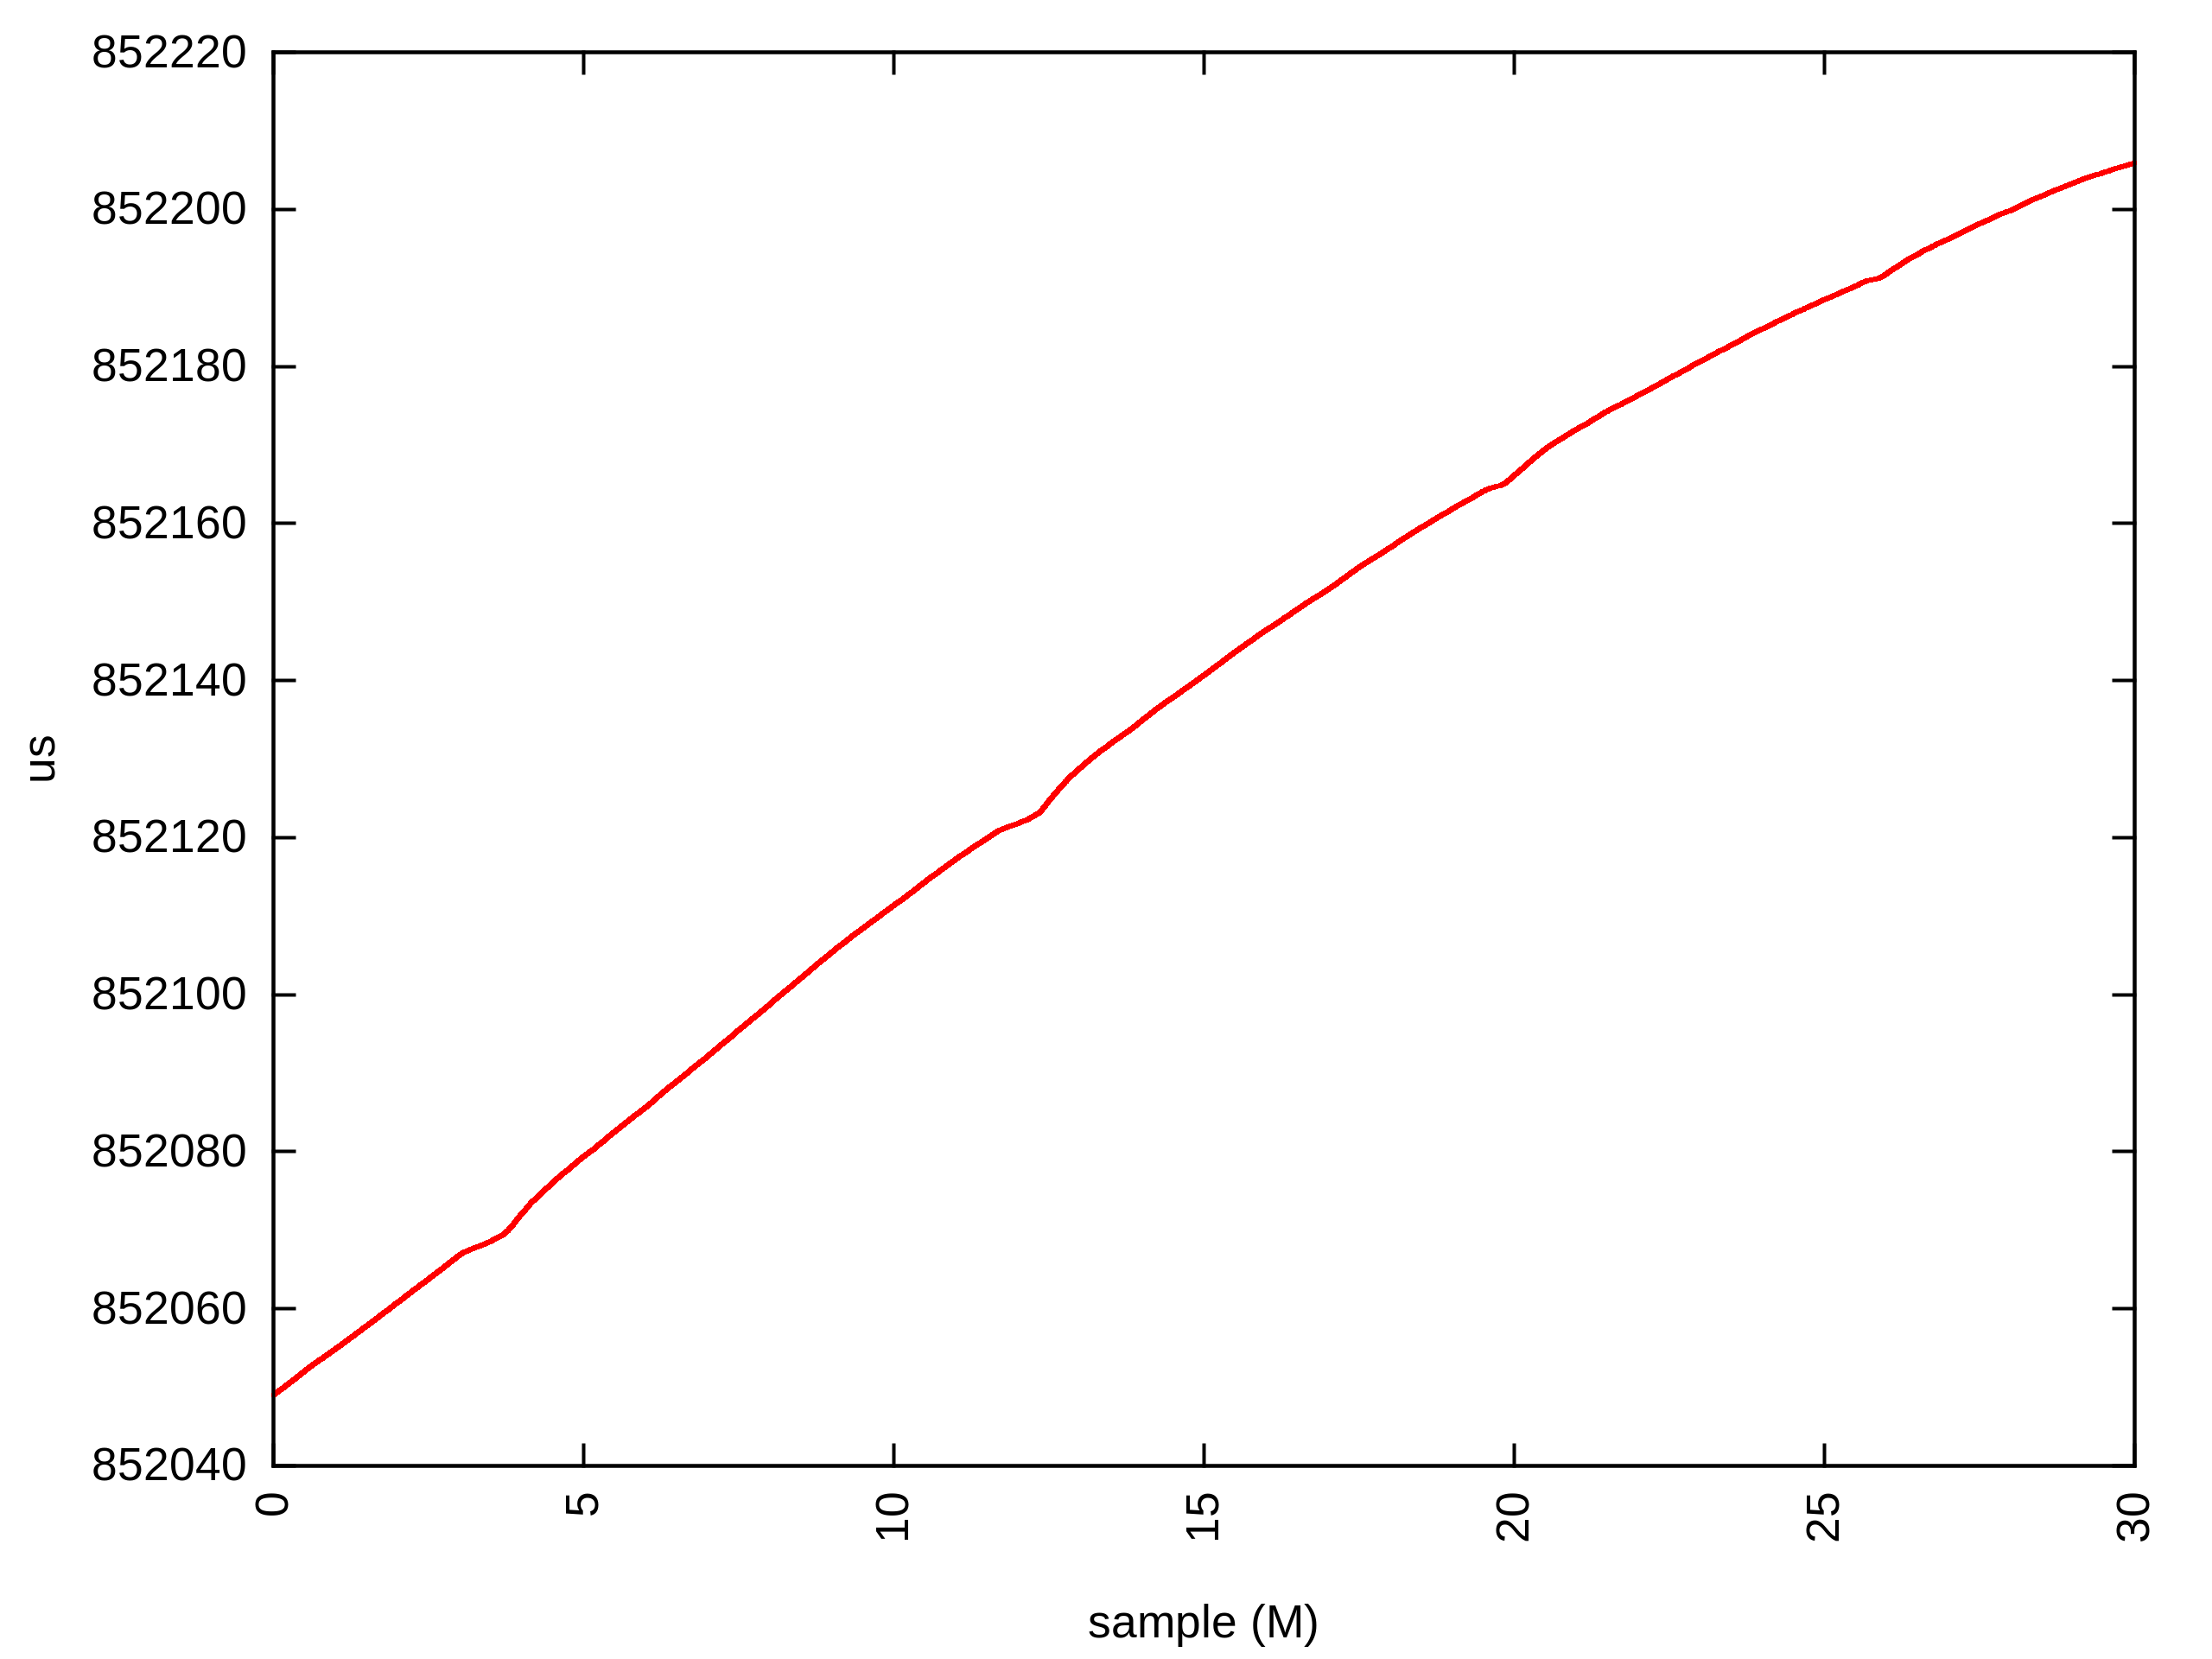
\includegraphics[width=0.80\textwidth]{img/test5_samples_absolute.png}
  \caption{Test 5: Acquired samples (absolute timestamps)}
  \label{test5_absolute}
\end{figure}

\begin{figure}[ht!]
  \centering
   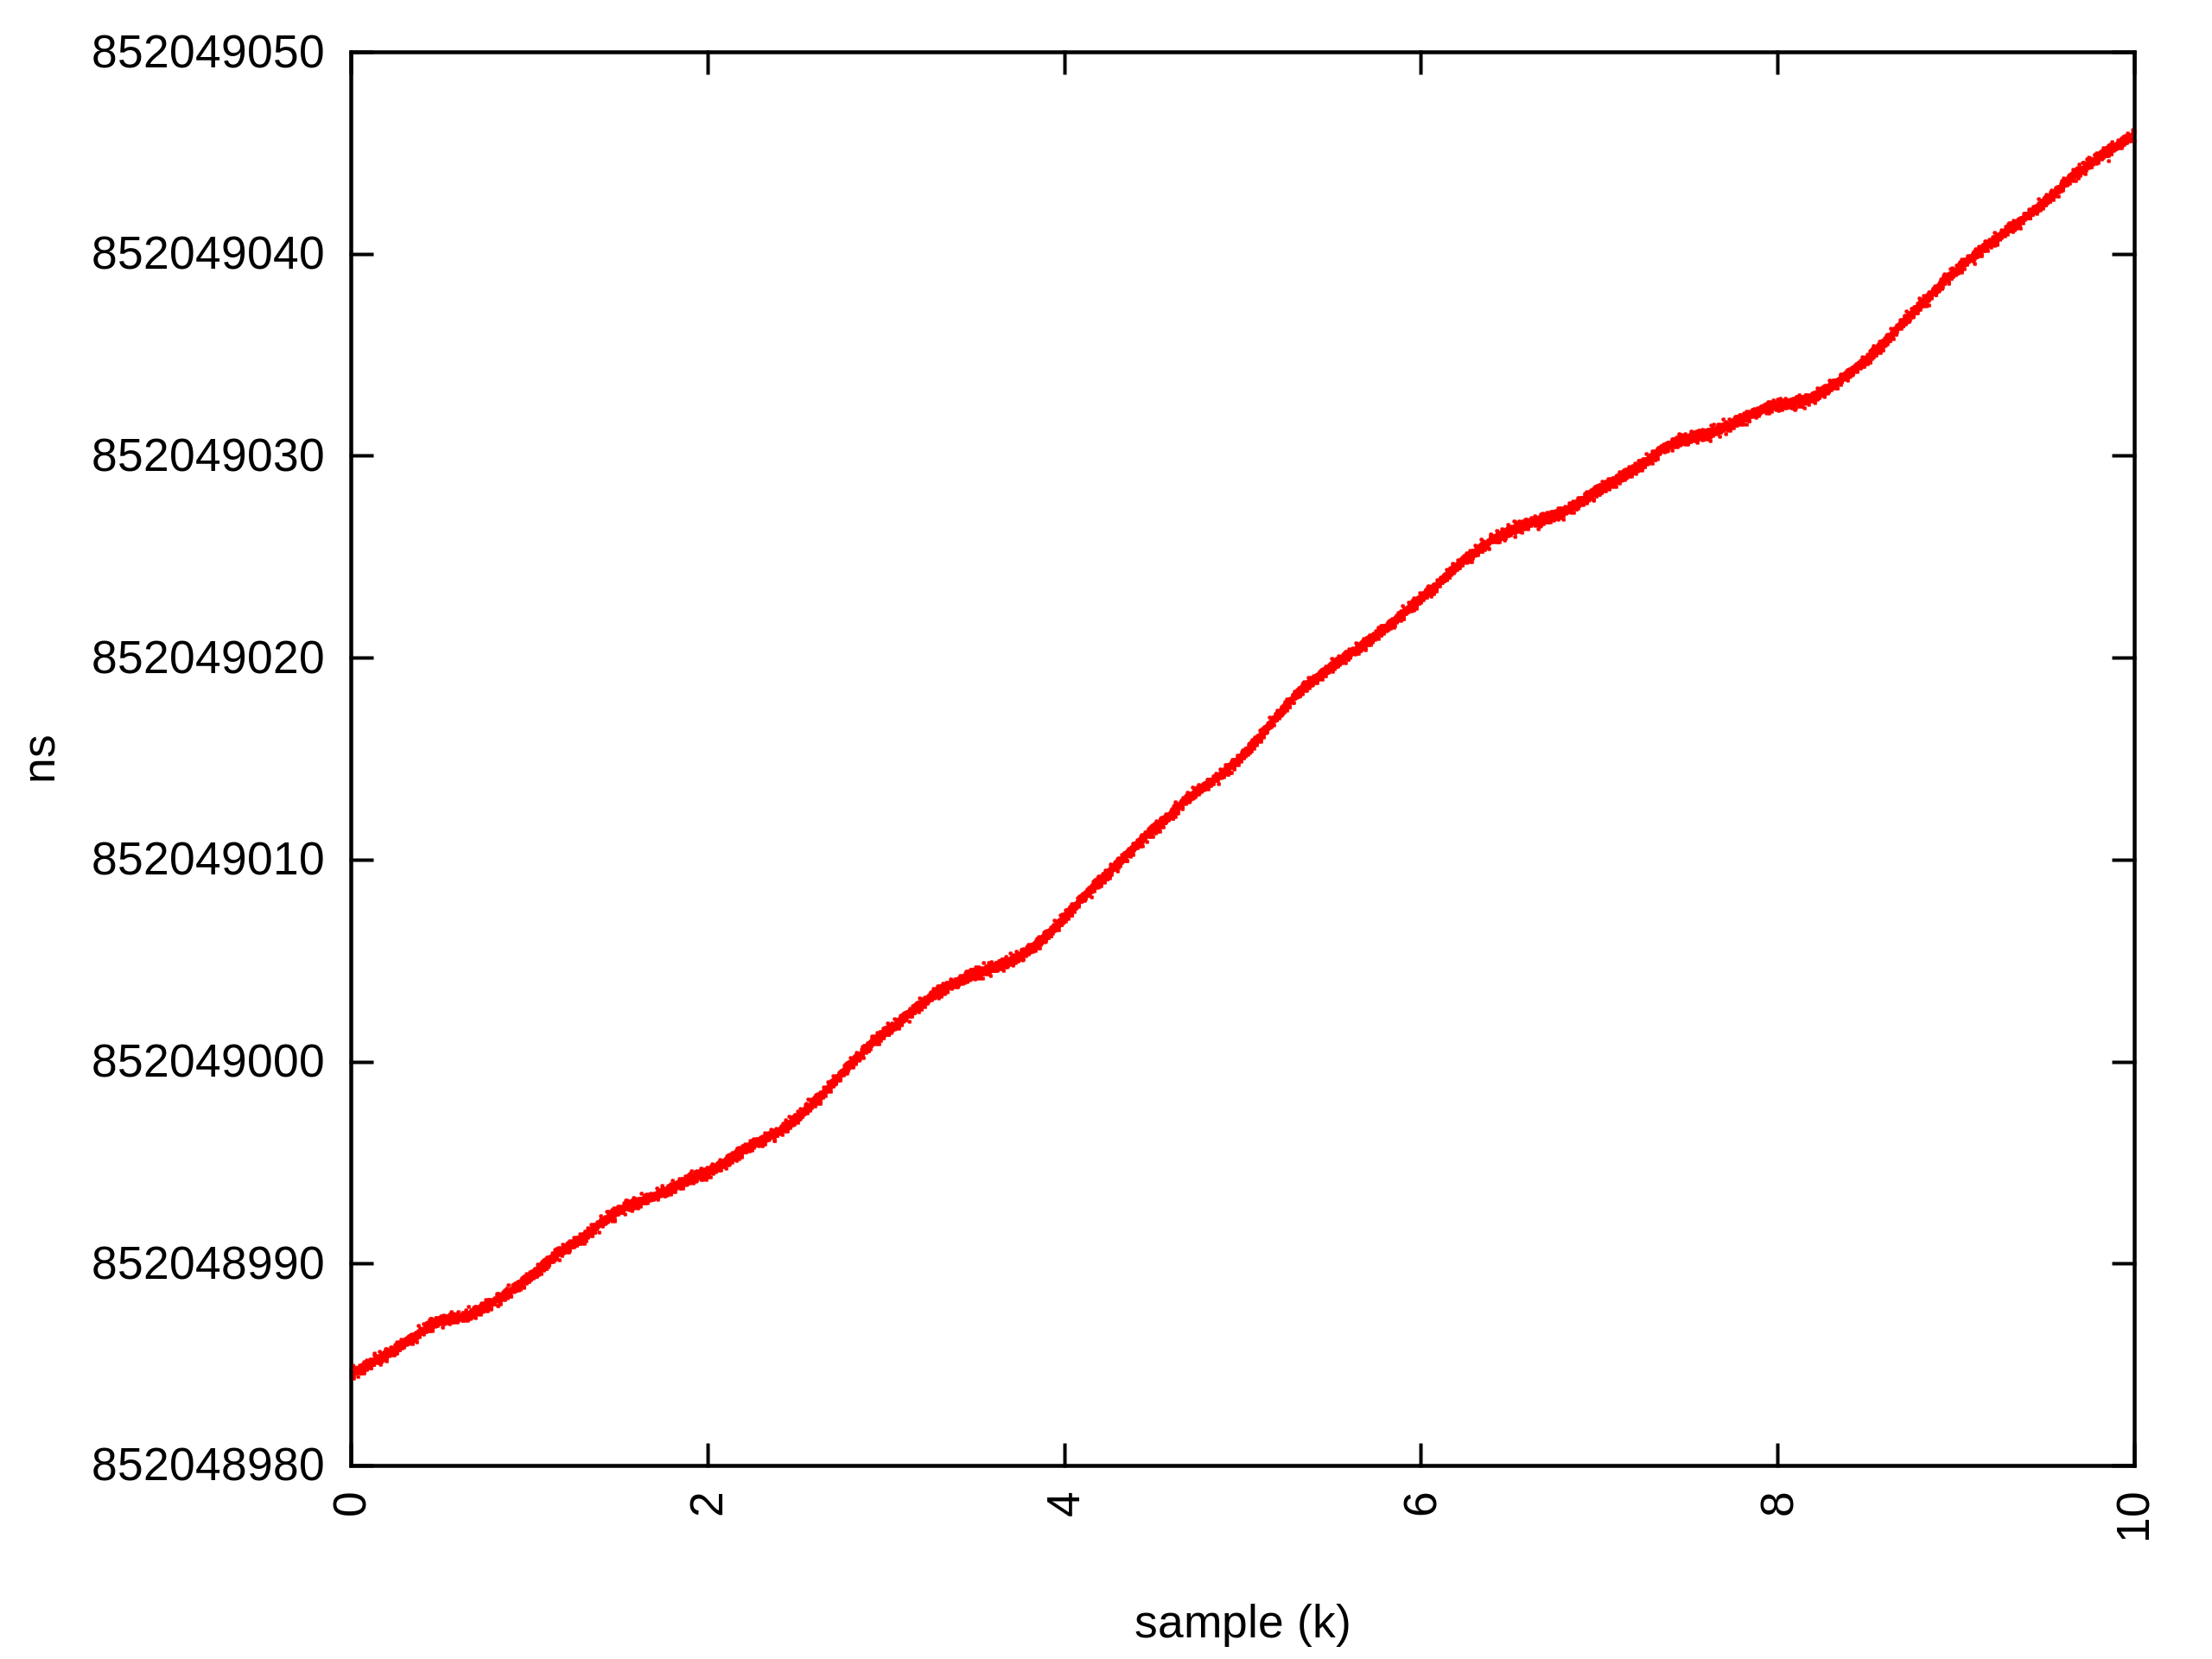
\includegraphics[width=0.80\textwidth]{img/test5_samples_absolute_zoom.png}
  \caption{Test 5: Subset of acquired samples (absolute timestamps)}
  \label{test5_absolute_zoom}
\end{figure}

Figures~\ref{test5_absolute} and~\ref{test5_absolute_zoom} show the absolute
timestamps of the data gathered during the run~1 of this test.
The data presented in the~Figure~\ref{test5_absolute} shows the continuous
drift of the local oscillator from the White Rabbit used as the reference on
the Fine-Delay board generating pulses.
If there were no drift, the line in the~Figure~\ref{test5_absolute} would be
horizontal (like in~Figure~\ref{test2_absolute} of \textit{Test~2}).
Additionally, It can be observed that the line in
the~Figure~\ref{test5_absolute} is not straight.
This is caused by the fluctuations of the drift of the local oscillator
compared to the White Rabbit.
Figure~\ref{test5_absolute_zoom} is the zoom in of the data presented in
the~Figure~\ref{test5_absolute}. It shows in details the mentioned fluctuations.

\FloatBarrier

\begin{figure}[ht!]
  \centering
  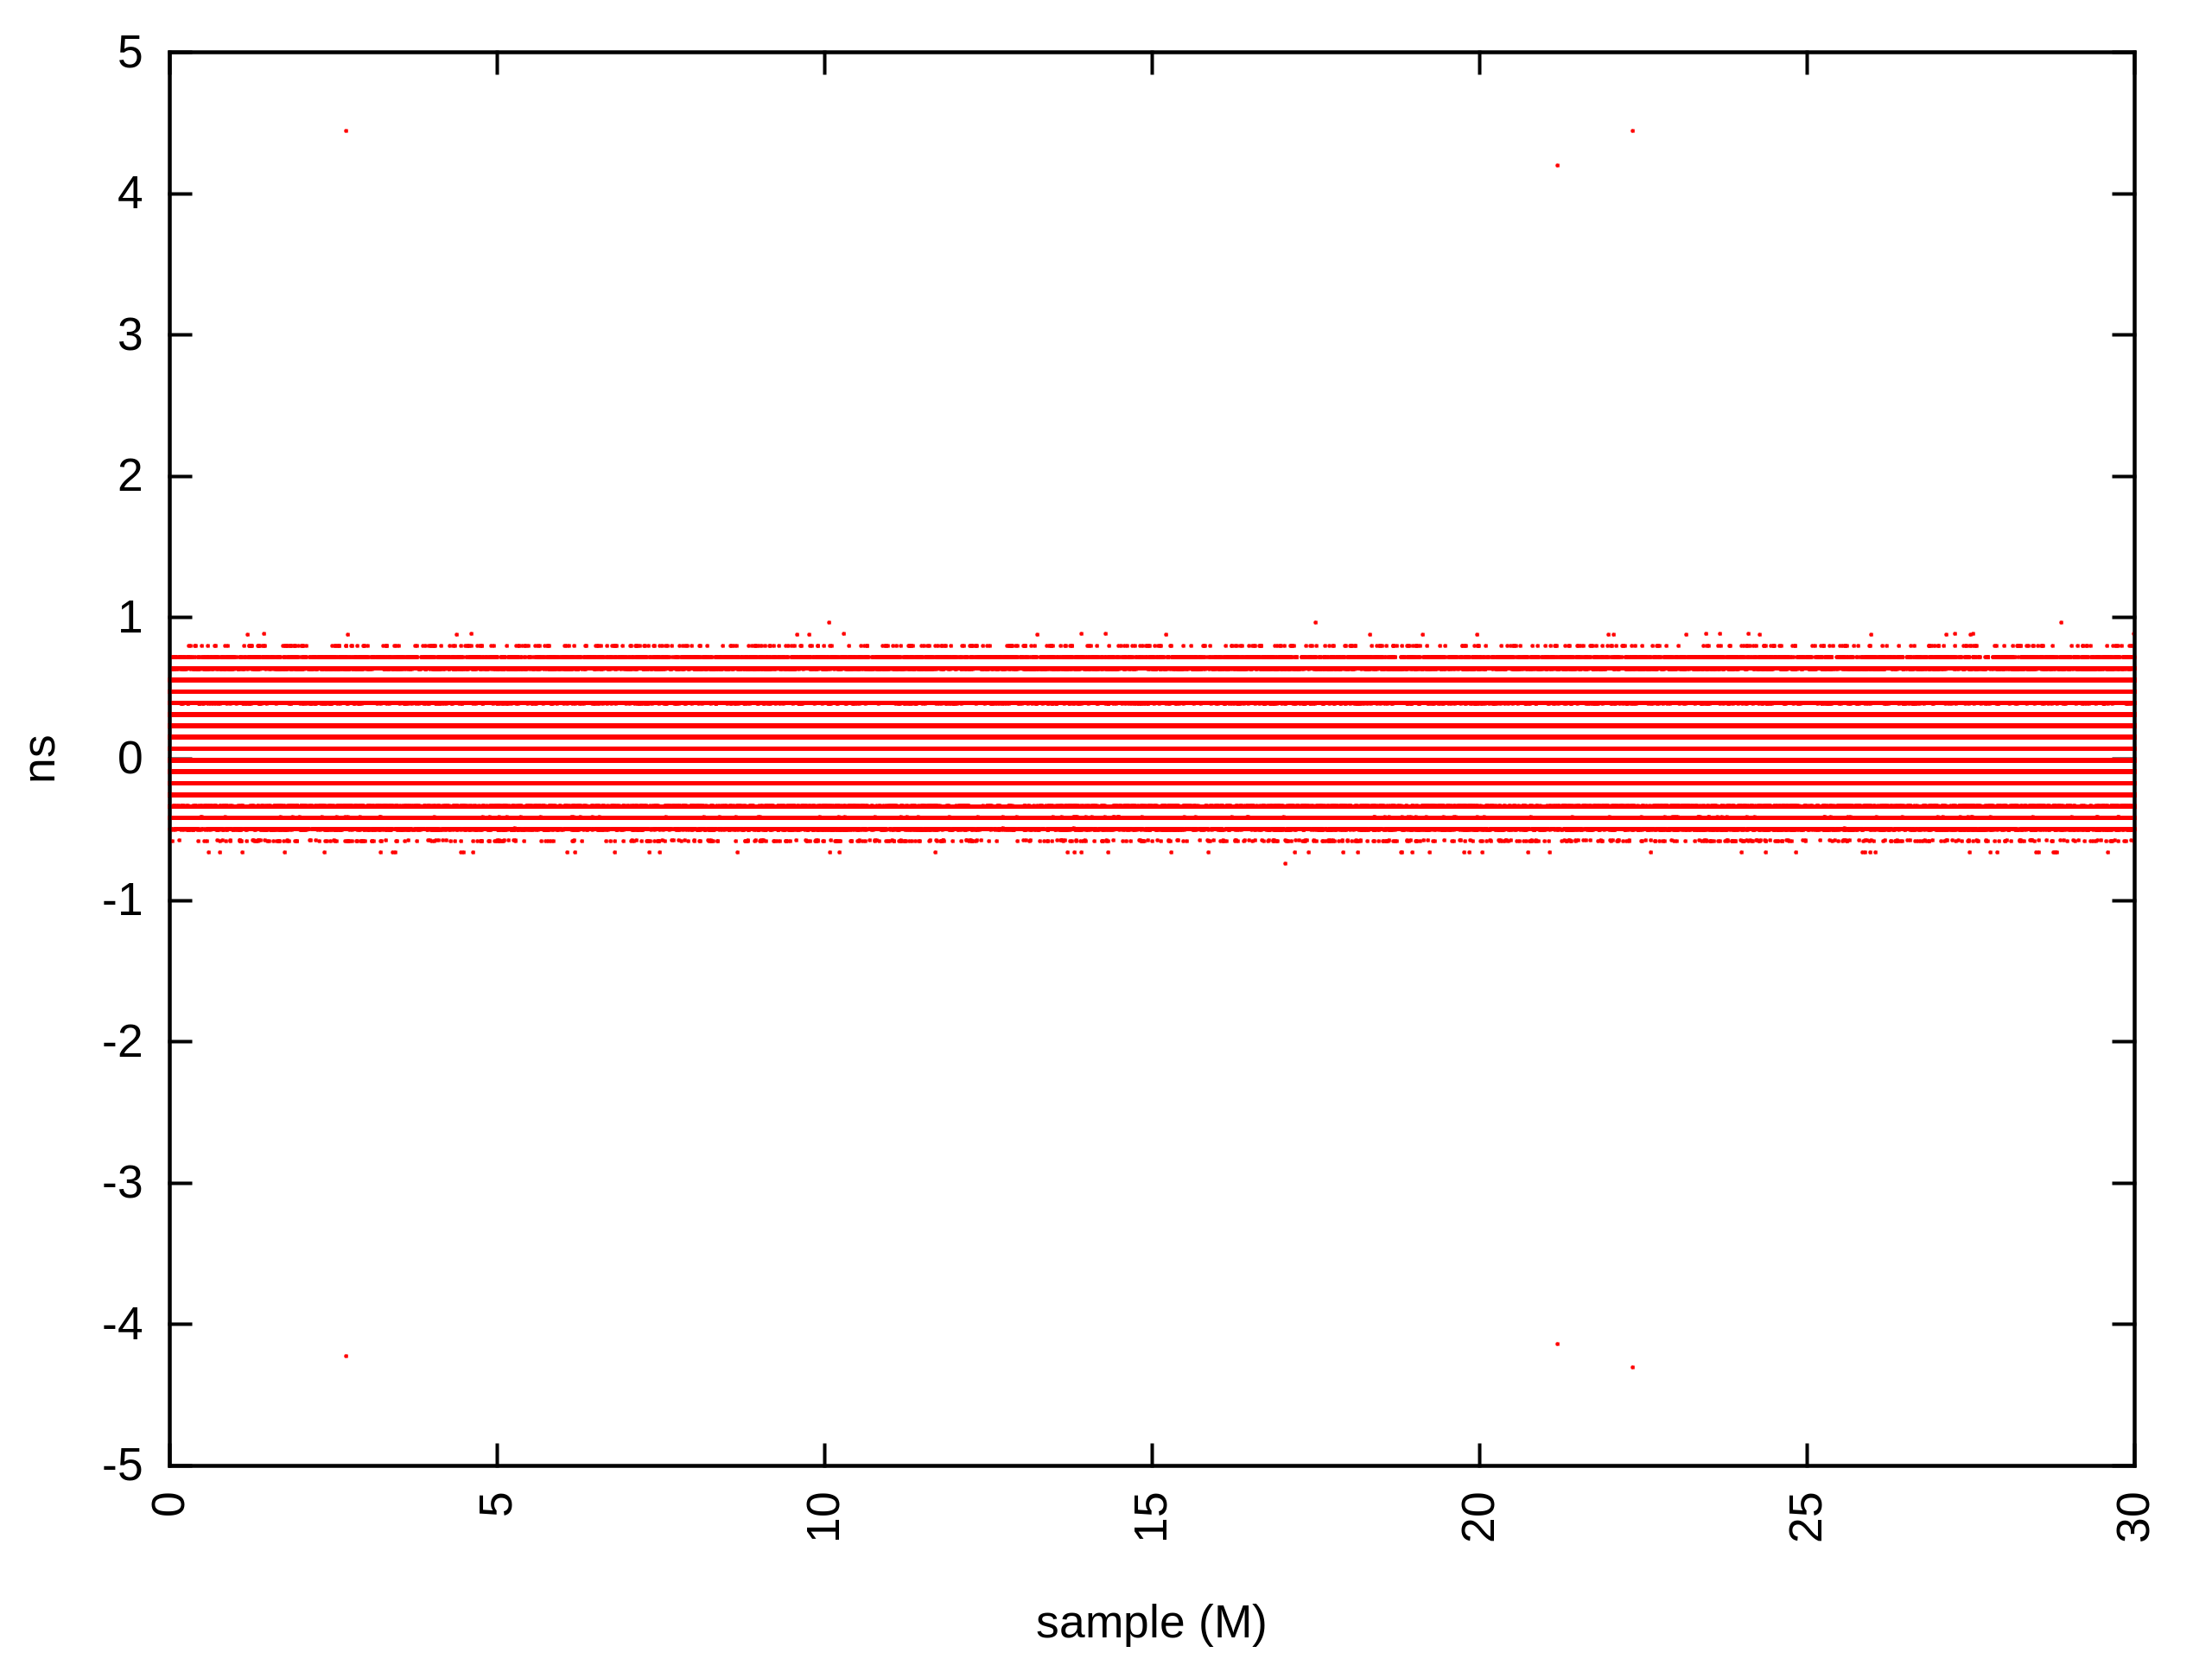
\includegraphics[width=0.8\textwidth]{img/test5_samples_relative.png}
  \caption{Test 5: Acquired samples (relative timestamps)}
  \label{test5_relative}
\end{figure}

\begin{figure}[ht!]
  \centering
  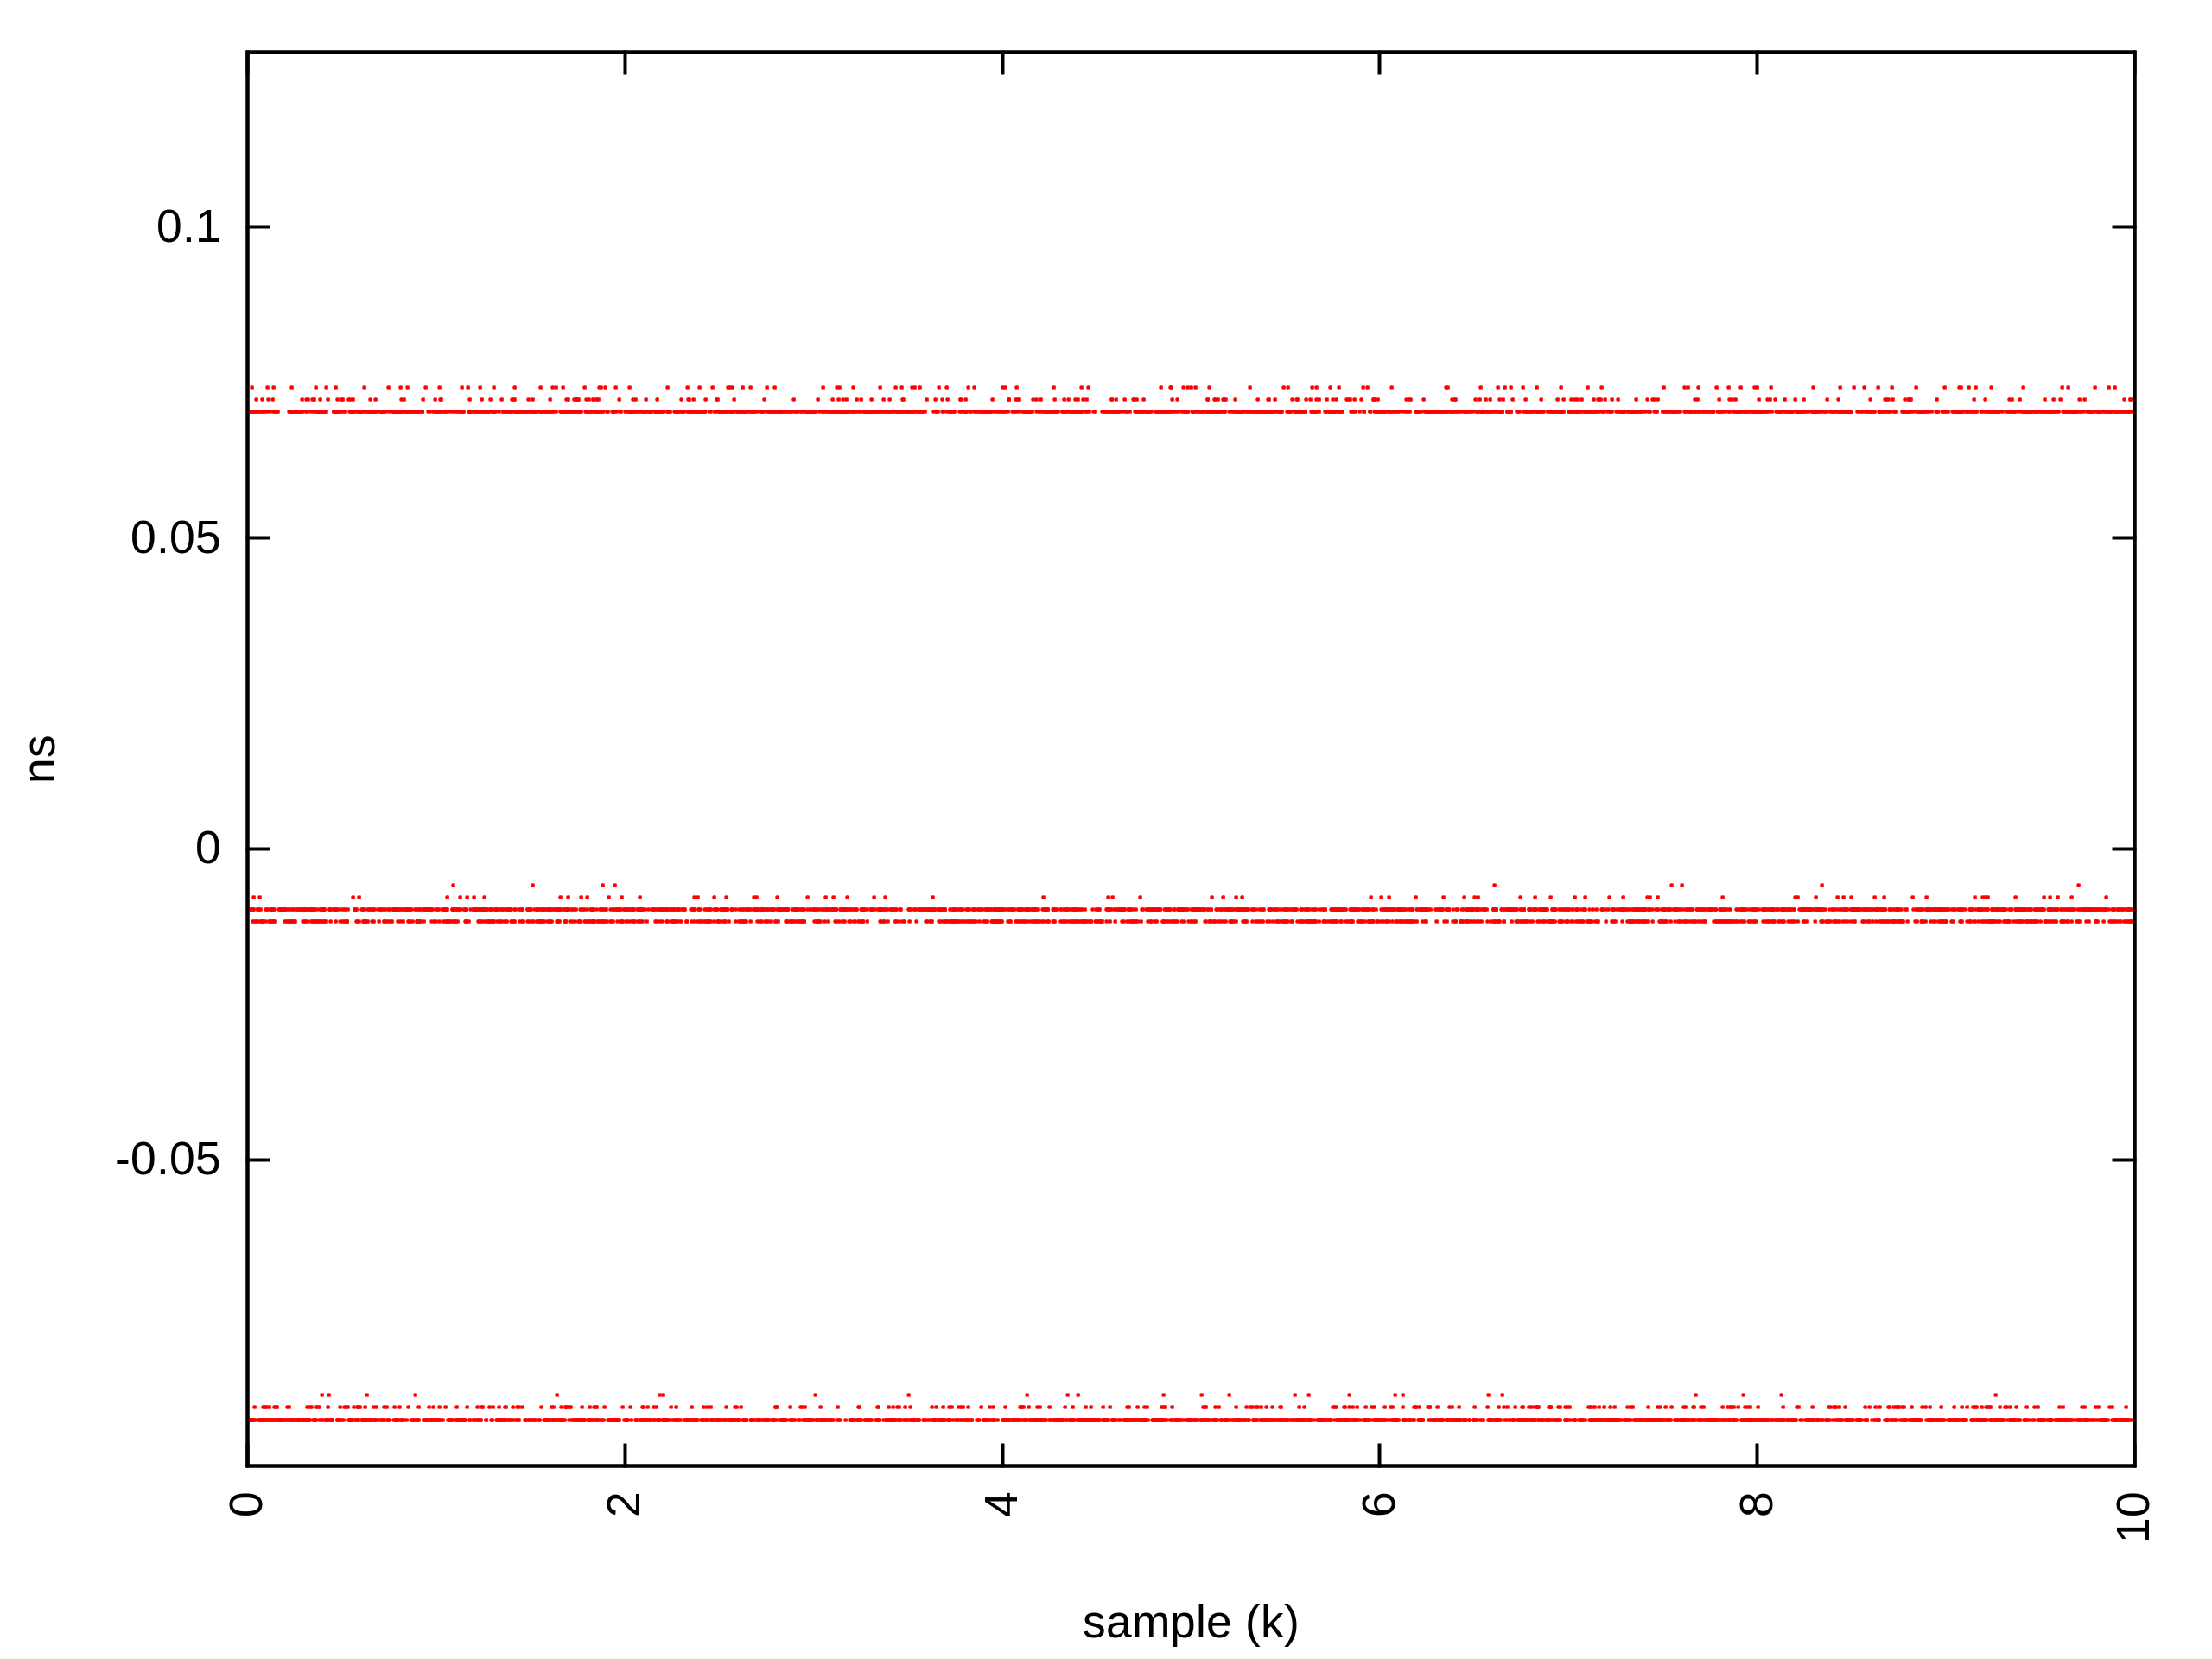
\includegraphics[width=0.7\textwidth]{img/test5_samples_relative_zoomxy.png}
  \caption{Test 5: Subset of acquired samples (relative timestamps)}
  \label{test5_relative_zoomy}
\end{figure}

The~Figure~\ref{test5_relative} shows the relative timestamps of the acquired
data.
A relative timestamp is a difference between a two consecutive timestamps
subtracted by one sample period.
The relative timestamps are arranged as several horizontal lines.
It is believed this quantization is due to the internal architecture of
the timestamping chip used on the TDC.
Zooming in the data presented in the~Figure~\ref{test5_relative} shows that each
line contains samples at few further levels (Figure~\ref{test5_relative_zoomy}).

\FloatBarrier
\begin{figure}[ht!]
  \centering
  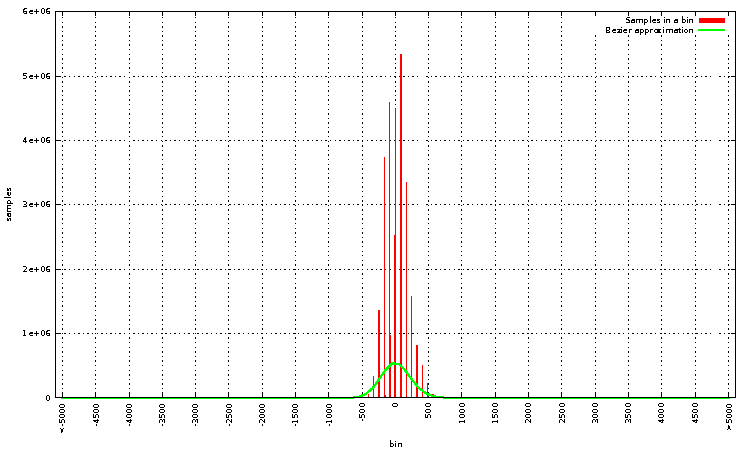
\includegraphics[width=0.80\textwidth]{img/test5_histogram.pdf}
  \caption{Test 5: Histogram of acquired samples (relative timestamps)}
  \label{test5_histogram}
\end{figure}

In the~Figure~\ref{test5_histogram}, the same as above relative samples are
presented in the form of histogram. The histogram is divided into 1000 bins.
Each bin spans over 10 ps.
Two additional bins were added to keep all values greater and smaller than
5000ps.

As a consequence of the distribution of samples shown in
the~Figure~\ref{test5_relative}, there are many empty bins between filled bins
(like gaps between lines in the mentioned figure).
To overcome quantization effect and to give better overview
the Bezier approximation is added to the histogram figure.

\begin{figure}[ht!]
  \centering
  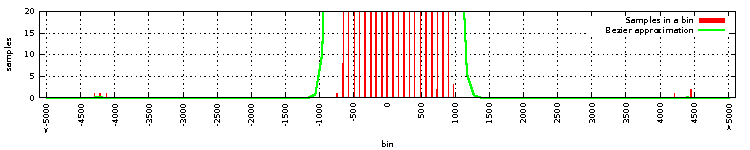
\includegraphics[width=1\textwidth]{img/test5_histogram_zoomy.pdf}
  \caption{Test 5: Histogram of acquired samples (relative timestamps), zoom in
           on the Y axis of the histogram (Figure~\ref{test5_histogram})}
  \label{test5_histogram_zoomy}
\end{figure}

Figure~\ref{test5_histogram_zoomy} shows the zoom in on the Y axis of
the histogram presented in the~Figure~\ref{test5_histogram}.
This shows that bins outside the center part of the figure are empty
(with the exception of few samples around $\pm$4ns, but this problem is
discussed later).

\begin{figure}[ht!]
  \centering
  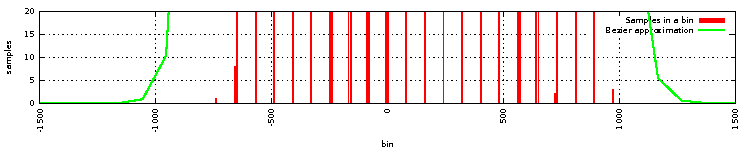
\includegraphics[width=1\textwidth]{img/test5_histogram_zoomx.pdf}
  \caption{Test 5: Histogram of acquired samples (relative timestamps),
           zoom in of the bottom center of the histograms
           (Figure~\ref{test5_histogram})}
  \label{test5_histogram_zoomx}
\end{figure}

Figure~\ref{test5_histogram_zoomx} shows the zoom in of the bottom center
part of the histogram presented in the~Figure~\ref{test5_histogram}.
It gives better view about number of samples placed in bins that are close to
the center of the histogram.
\FloatBarrier

Statistical summary of several runs of the \textit{Test~5} is presented in
the Table~\ref{table_test5_summary}.

\begin{table}[!htb]
  \centering
  \footnotesize
  \begin{tabular}{|c|r|r|r|r|r|r|}
    \hline {\bf Run} & {\bf Data Volume} & {\bf Mean (ps)} & {\bf Sigma (ps)} & {\bf Min (ps)} & {\bf Max (ps)} & {\bf Range (ps)}  \\
    \hline
    1                &               30M &           5.230 &          155.821 &      -4304.688 &       4445.312 &          8750.000 \\
    ** 1             &               30M &           5.230 &          155.809 &       -740.234 &        964.844 &          1705.078 \\
    2                &               30M &          -4.892 &          156.068 &      -4384.766 &       4363.281 &          8748.047 \\
    ** 2             &               30M &          -4.892 &          156.056 &       -660.156 &        964.844 &          1625.000 \\
    3                &              100M &          -5.022 &          154.184 &      -4546.875 &       4771.484 &          9318.359 \\
    **3              &              100M &          -5.022 &          154.174 &       -660.156 &       1044.922 &          1705.078 \\
    4                &               30M &         -13.113 &          155.214 &       -740.234 &        884.766 &          1625.000 \\
    \hline
  \end{tabular}
  \caption{Summary of \textit{Test~5} runs}
  \label{table_test5_summary}
\end{table}

In the run 1, 2 and 3 there were samples that significantly differed from
other values. As mentioned before, it is suspected that this is the same issue
as described in~\cite{tdc_perf_test}.
The table~\ref{table_test5_summary}
includes the calculations for the same runs (marked with asterisk),
but without suspected timestamps. The Table~\ref{table_test5_samples_excluded}
includes the details about the excluded values.

\begin{table}[!htb]
  \centering
  \tiny
  \begin{tabular}{|r|r|r|}
    \hline
    {\bf run } &{\bf sample \#} & {\bf Delta (ps)} \\
    \hline
    1          & 2693502  &  4445.312500   \\
    1          & 2693503  & -4222.656250   \\
    1          & 21186672 & -4138.671875   \\
    1          & 21186673 &  4201.171875   \\
    1          & 22336621 &  4445.312500   \\
    1          & 22336622 & -4304.687500   \\
    2          &  8400423 &  4283.203125   \\
    2          &  8400424 & -4384.765625   \\
    2          & 22158883 &  4363.281250   \\
    2          & 22158884 & -4218.750000   \\
    2          & 26818627 &  4203.125000   \\
    2          & 26818628 & -4304.687500   \\
    3          & 6445599  &  4363.281250   \\
    3          & 6445600  & -4304.687500   \\
    3          & 34262007 &  4771.484375   \\
    3          & 34262008 & -4546.875000   \\
    3          & 50023335 &  4283.203125   \\
    3          & 50023336 & -4304.687500   \\
    3          & 65164383 &  4445.312500   \\
    3          & 65164384 & -4466.796875   \\
    3          & 65517181 &  4525.390625   \\
    3          & 65517182 & -4544.921875   \\
    3          & 76384109 & -4222.656250   \\
    3          & 76384110 &  4363.281250   \\
    3          & 87556693 &  4691.406250   \\
    3          & 87556694 & -4464.843750   \\
    3          & 92080941 &  4281.250000   \\
    3          & 92080942 & -4140.625000   \\
    \hline
  \end{tabular}
  \caption{Samples excluded from calculations of \textit{Test~5} runs}
  \label{table_test5_samples_excluded}
\end{table}


% 1:
% 0x5:2 2693502  0.85206496502929685022  0.00000000444531250000   0.00000000444531250000 seq: 2693502 timestamp: 3248.354065 raw: 00000cb0:02a35348:00000a0f, debug: 029197ea
% 0x5:2 2693503  0.85206496080664062553 -0.00000000422265625000  -0.00000000422265625000 seq: 2693503 timestamp: 3248.355065 raw: 00000cb0:02a53b90:0000019d, debug: 029197fa
% 0x5:2 21186672  0.85217277628515619714 -0.00000000413867187500 -0.00000000413867187500 seq: 21186672 timestamp: 21741.524173 raw: 000054ed:03e7c7bd:00000092, debug: 1434870a
% 0x5:2 21186673  0.85217278048632816301  0.00000000420117187500  0.00000000420117187500 seq: 21186673 timestamp: 21741.525173 raw: 000054ed:03e9b005:000008f9, debug: 1434871a
% 0x5:2 22336621  0.85217775480859370152  0.00000000444531250000  0.00000000444531250000 seq: 22336621 timestamp: 22891.473178 raw: 0000596b:038683d3:0000059e, debug: 154d46da
% 0x5:2 22336622  0.85217775050390620617 -0.00000000430468750000 -0.00000000430468750000 seq: 22336622 timestamp: 22891.474178 raw: 0000596b:03886c1a:00000d02, debug: 154d46ea

% 2:
% 0x5:2  8400423 -0.94059297612109371567  0.00000000428320312500  0.00000000428320312500 seq: 8400423 timestamp: 8400.482407 raw: 000020d0:03981e4d:00000fc2, debug: 0802e27a
% 0x5:2  8400424 -0.94059298050585937734 -0.00000000438476562500 -0.00000000438476562500 seq: 8400424 timestamp: 8400.483407 raw: 000020d0:039a0695:000006fd, debug: 0802e28a
% 0x5:2 22158883 -0.94066104980859377438  0.00000000436328125000  0.00000000436328125000 seq: 22158883 timestamp: 22158.942339 raw: 0000568e:07055e70:00000c62, debug: 1521e23a
% 0x5:2 22158884 -0.94066105402734379037 -0.00000000421875000000 -0.00000000421875000000 seq: 22158884 timestamp: 22158.943339 raw: 0000568e:070746b8:000003f2, debug: 1521e24a
% 0x5:2 26818627 -0.94068755157617189866  0.00000000420312500000  0.00000000420312500000 seq: 26818627 timestamp: 26818.686312 raw: 000068c2:051d0980:000000d9, debug: 1993843a
% 0x5:2 26818628 -0.94068755588085939401 -0.00000000430468750000 -0.00000000430468750000 seq: 26818628 timestamp: 26818.687312 raw: 000068c2:051ef1c7:0000083d, debug: 1993844a

%3:
% 0x5:2 6445599 -0.48455468271679685843   0.00000000436328125000  0.00000000436328125000 seq: 6445599 timestamp: 6446.114445 raw: 0000192e:00da4980:00000a91, debug: 0625a1fa
% 0x5:2 6445600 -0.48455468702148435378  -0.00000000430468750000 -0.00000000430468750000 seq: 6445600 timestamp: 6446.115445 raw: 0000192e:00dc31c8:000001f5, debug: 0625a20a
% 0x5:2 34262007 -0.48464741311718750882  0.00000000477148437500  0.00000000477148437500 seq: 34262007 timestamp: 34262.522353 raw: 000085d6:03e44ef9:000005c4, debug: 20acbf7a
% 0x5:2 34262008 -0.48464741766406249646 -0.00000000454687500000 -0.00000000454687500000 seq: 34262008 timestamp: 34262.523353 raw: 000085d6:03e63740:00000cac, debug: 20acbf8a
% 0x5:2 50023335 -0.48472851307617187411  0.00000000428320312500  0.00000000428320312500 seq: 50023335 timestamp: 50023.850271 raw: 0000c367:0655c39f:00000dd9, debug: 2fb4ba7a
% 0x5:2 50023336 -0.48472851738085936946 -0.00000000430468750000 -0.00000000430468750000 seq: 50023336 timestamp: 50023.851271 raw: 0000c367:0657abe7:0000053d, debug: 2fb4ba8a
% 0x5:2 65164383 -0.48480347421679687026  0.00000000444531250000  0.00000000444531250000 seq: 65164383 timestamp: 65164.898197 raw: 0000fe8c:06b12c85:00000b91, debug: 3e2545fa
% 0x5:2 65164384 -0.48480347868359374708 -0.00000000446679687500 -0.00000000446679687500 seq: 65164384 timestamp: 65164.899197 raw: 0000fe8c:06b314cd:000002a2, debug: 3e25460a
% 0x5:2 65517181 -0.48480588410546876510  0.00000000452539062500  0.00000000452539062500 seq: 65517181 timestamp: 65517.696194 raw: 0000ffed:052fe288:000007ca, debug: 3e7b67da
% 0x5:2 65517182 -0.48480588865039064839 -0.00000000454492187500 -0.00000000454492187500 seq: 65517182 timestamp: 65517.697194 raw: 0000ffed:0531cacf:00000eb3, debug: 3e7b67ea
% 0x5:2 76384109 -0.48488419337499999440 -0.00000000422265625000 -0.00000000422265625000 seq: 76384109 timestamp: 76384.624116 raw: 00012a60:04a6680b:00000d40, debug: 48d876da
% 0x5:2 76384110 -0.48488418901171875808  0.00000000436328125000  0.00000000436328125000 seq: 76384110 timestamp: 76384.625116 raw: 00012a60:04a85054:000005fa, debug: 48d876ea
% 0x5:2 87556693 -0.48497392305468750573  0.00000000469140625000  0.00000000469140625000 seq: 87556693 timestamp: 87557.208026 raw: 00015605:018cc73b:000009e4, debug: 5380255a
% 0x5:2 87556694 -0.48497392751953122270 -0.00000000446484375000 -0.00000000446484375000 seq: 87556694 timestamp: 87557.209026 raw: 00015605:018eaf83:000000f6, debug: 5380256a
% 0x5:2 92080941 -0.48500224157421872873  0.00000000428125000000  0.00000000428125000000 seq: 92080941 timestamp: 92081.455998 raw: 000167b1:0365bf27:00000cda, debug: 57d0b2da
% 0x5:2 92080942 -0.48500224571484373826 -0.00000000414062500000 -0.00000000414062500000 seq: 92080942 timestamp: 92081.456998 raw: 000167b1:0367a76f:00000492, debug: 57d0b2ea

The mean value of samples within a run differs between runs due to the drift
of the local oscillator with the reference to White Rabbit used on
the pulse generator. The other values seam to be stable between different runs.

To gather all data in the described test, the following python command has been
used:
\begin{lstlisting}
$ python -d -m pytest  test_fmctdc_acquisition.py::\
  TestFmctdcAcquisition::test_acq_timestamp_multiple_hist --usr-acq-count=100000000 \
  --usr-acq-period-ns=1000000 --tdc-id-ch 0x5:2 \
  --samples-file test4_sample --histogram-file test5_hist \
  --bin-min-ps -5000 --bin-max-ps 5000 --bins-num 1000 --tdc-wr-off
\end{lstlisting}

\FloatBarrier

\subsection{Test 6}
\label{test6}
Test summary:
\begin{center}
  \begin{tabular}{|l|l|}
    \hline {\bf Test parameter} & {\bf Value} \\
    \hline
    Pulse frequency                      & 1kHz  \\
    Pulse width                          & 1000ns \\
    Test duration                        & 27h \\
    Number of samples                    & 100M \\
    Clock reference                      & White Rabbit \\
    \hline
  \end{tabular}
\end{center}

This test is very similar to the~\textit{Test 5} described in
subsection~\ref{test5}.
However, in this test the TDC uses White Rabbit as a time reference
instead of the local oscillator.

\begin{figure}[ht!]
  \centering
  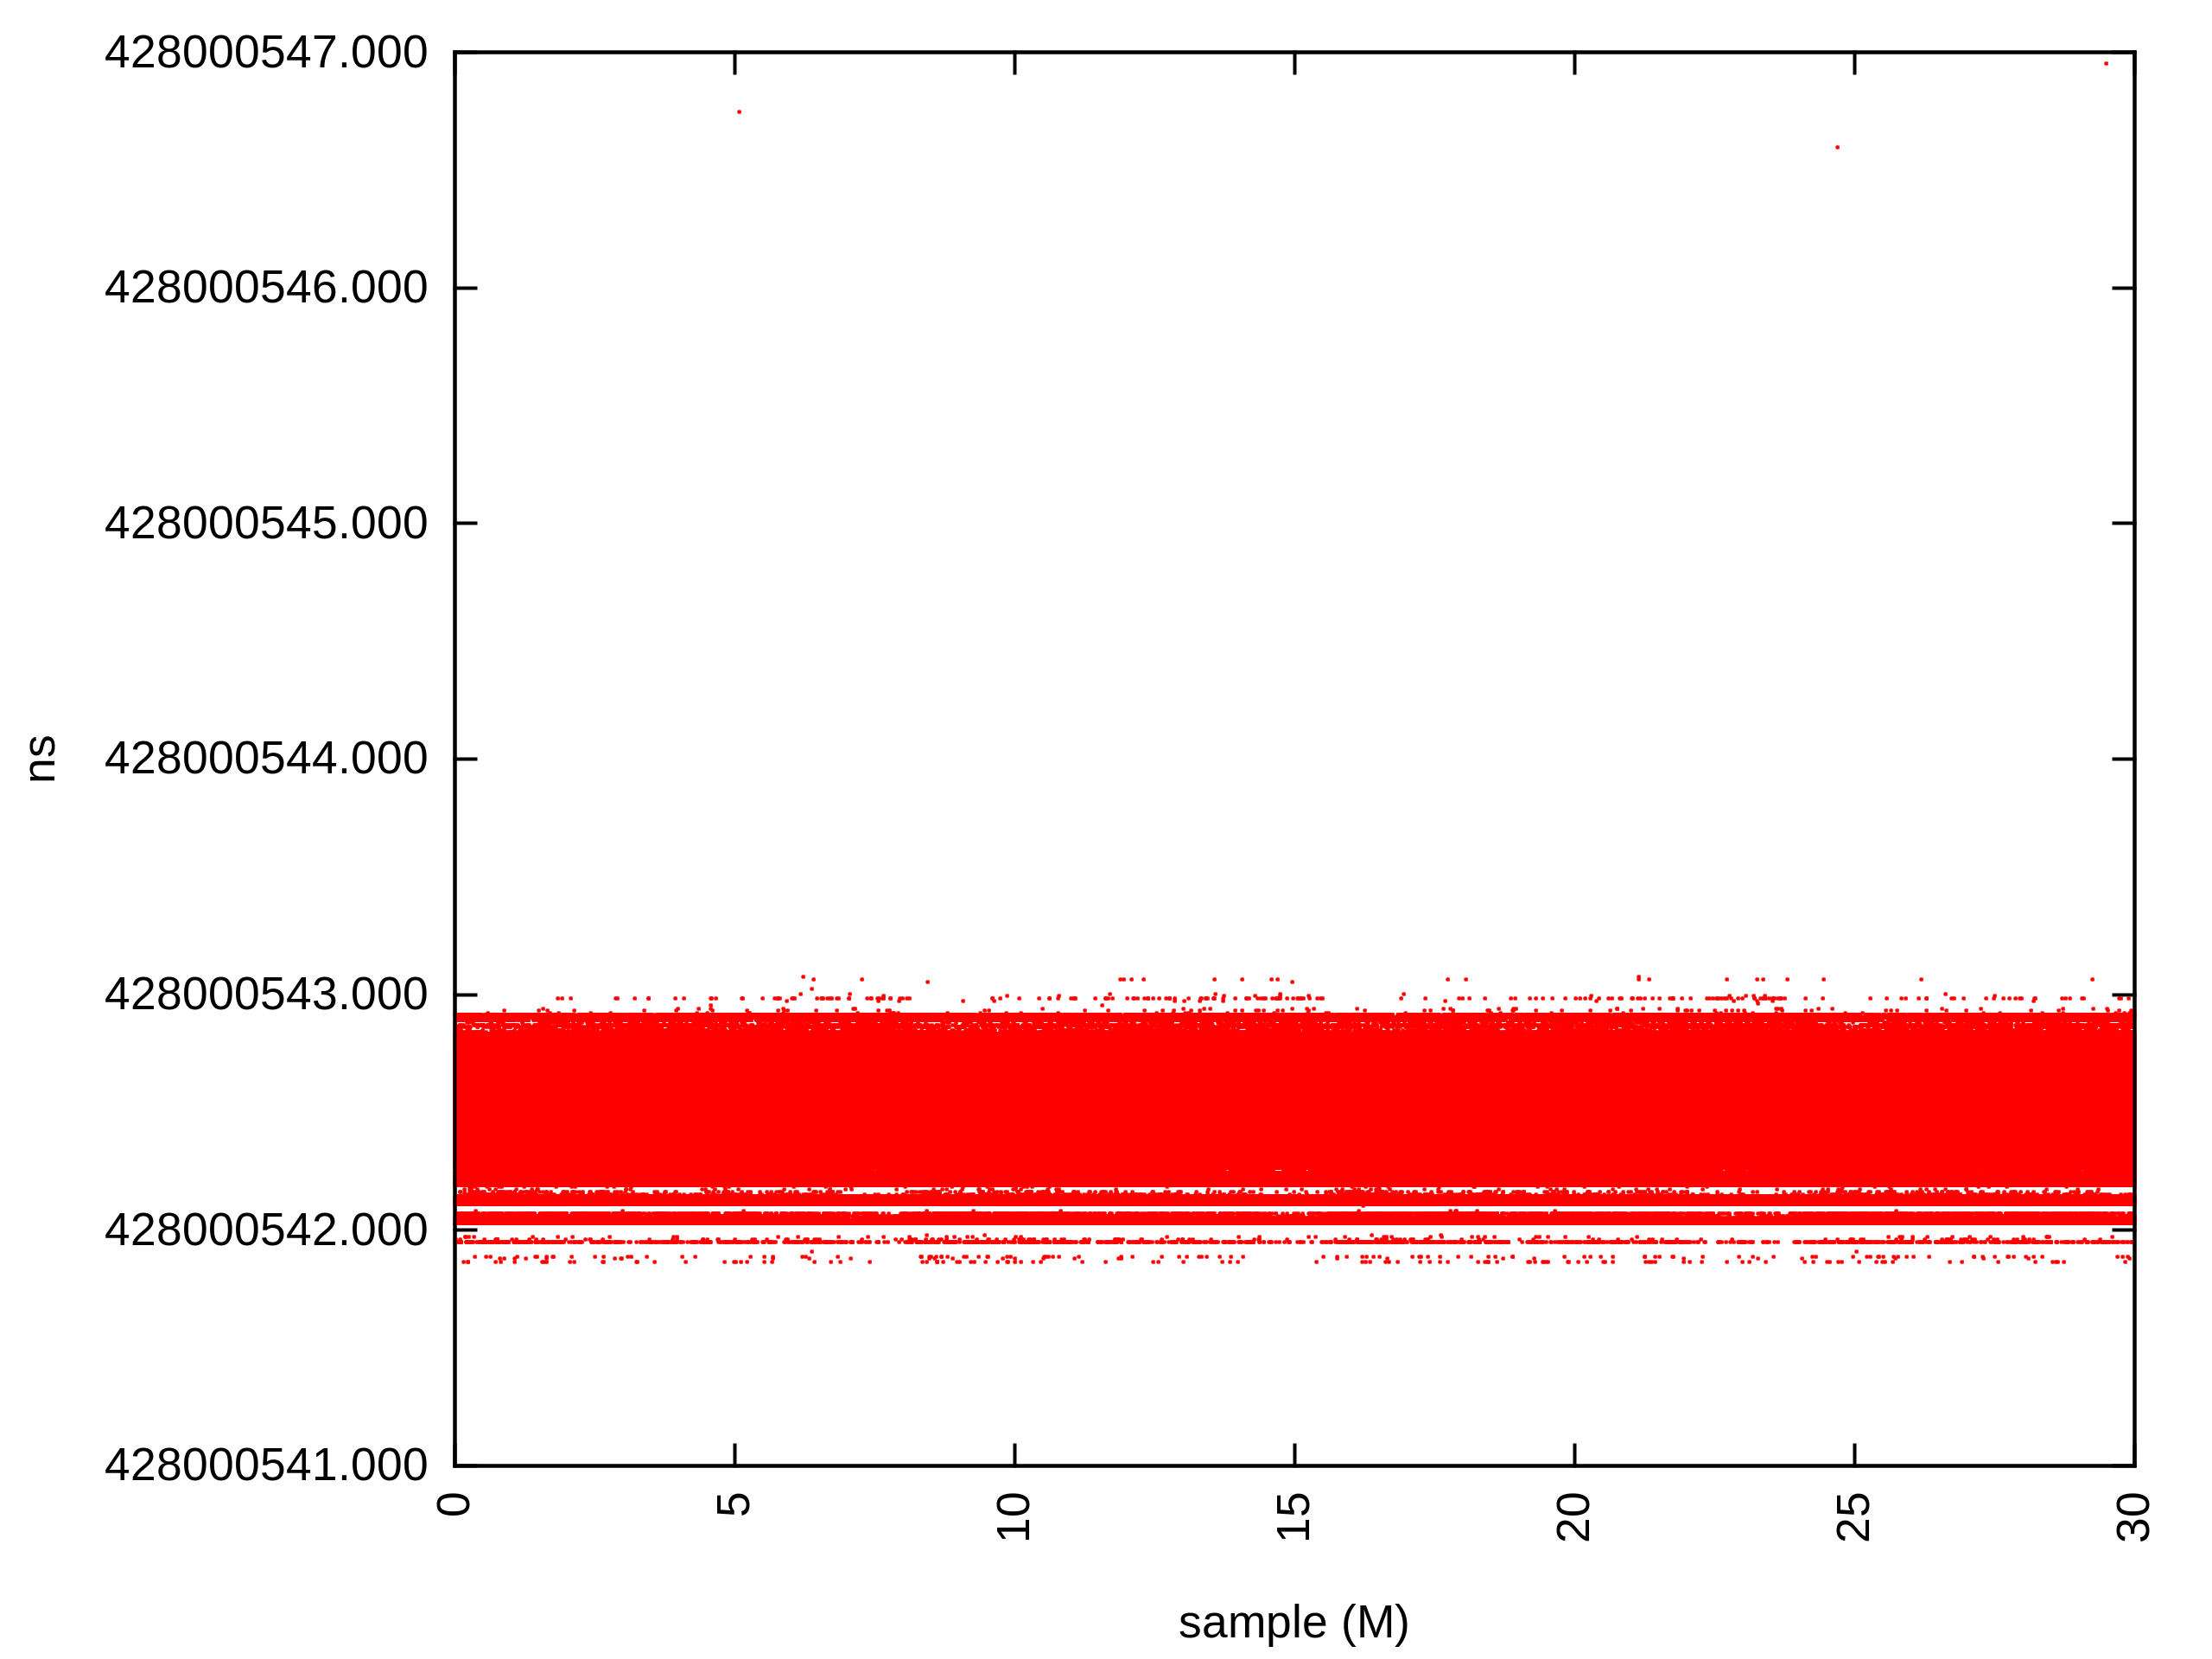
\includegraphics[width=0.80\textwidth]{img/test6_samples_absolute.png}
  \caption{Test 6: Acquired samples (absolute timestamps)}
  \label{test6_absolute}
\end{figure}

\begin{figure}[ht!]
  \centering
  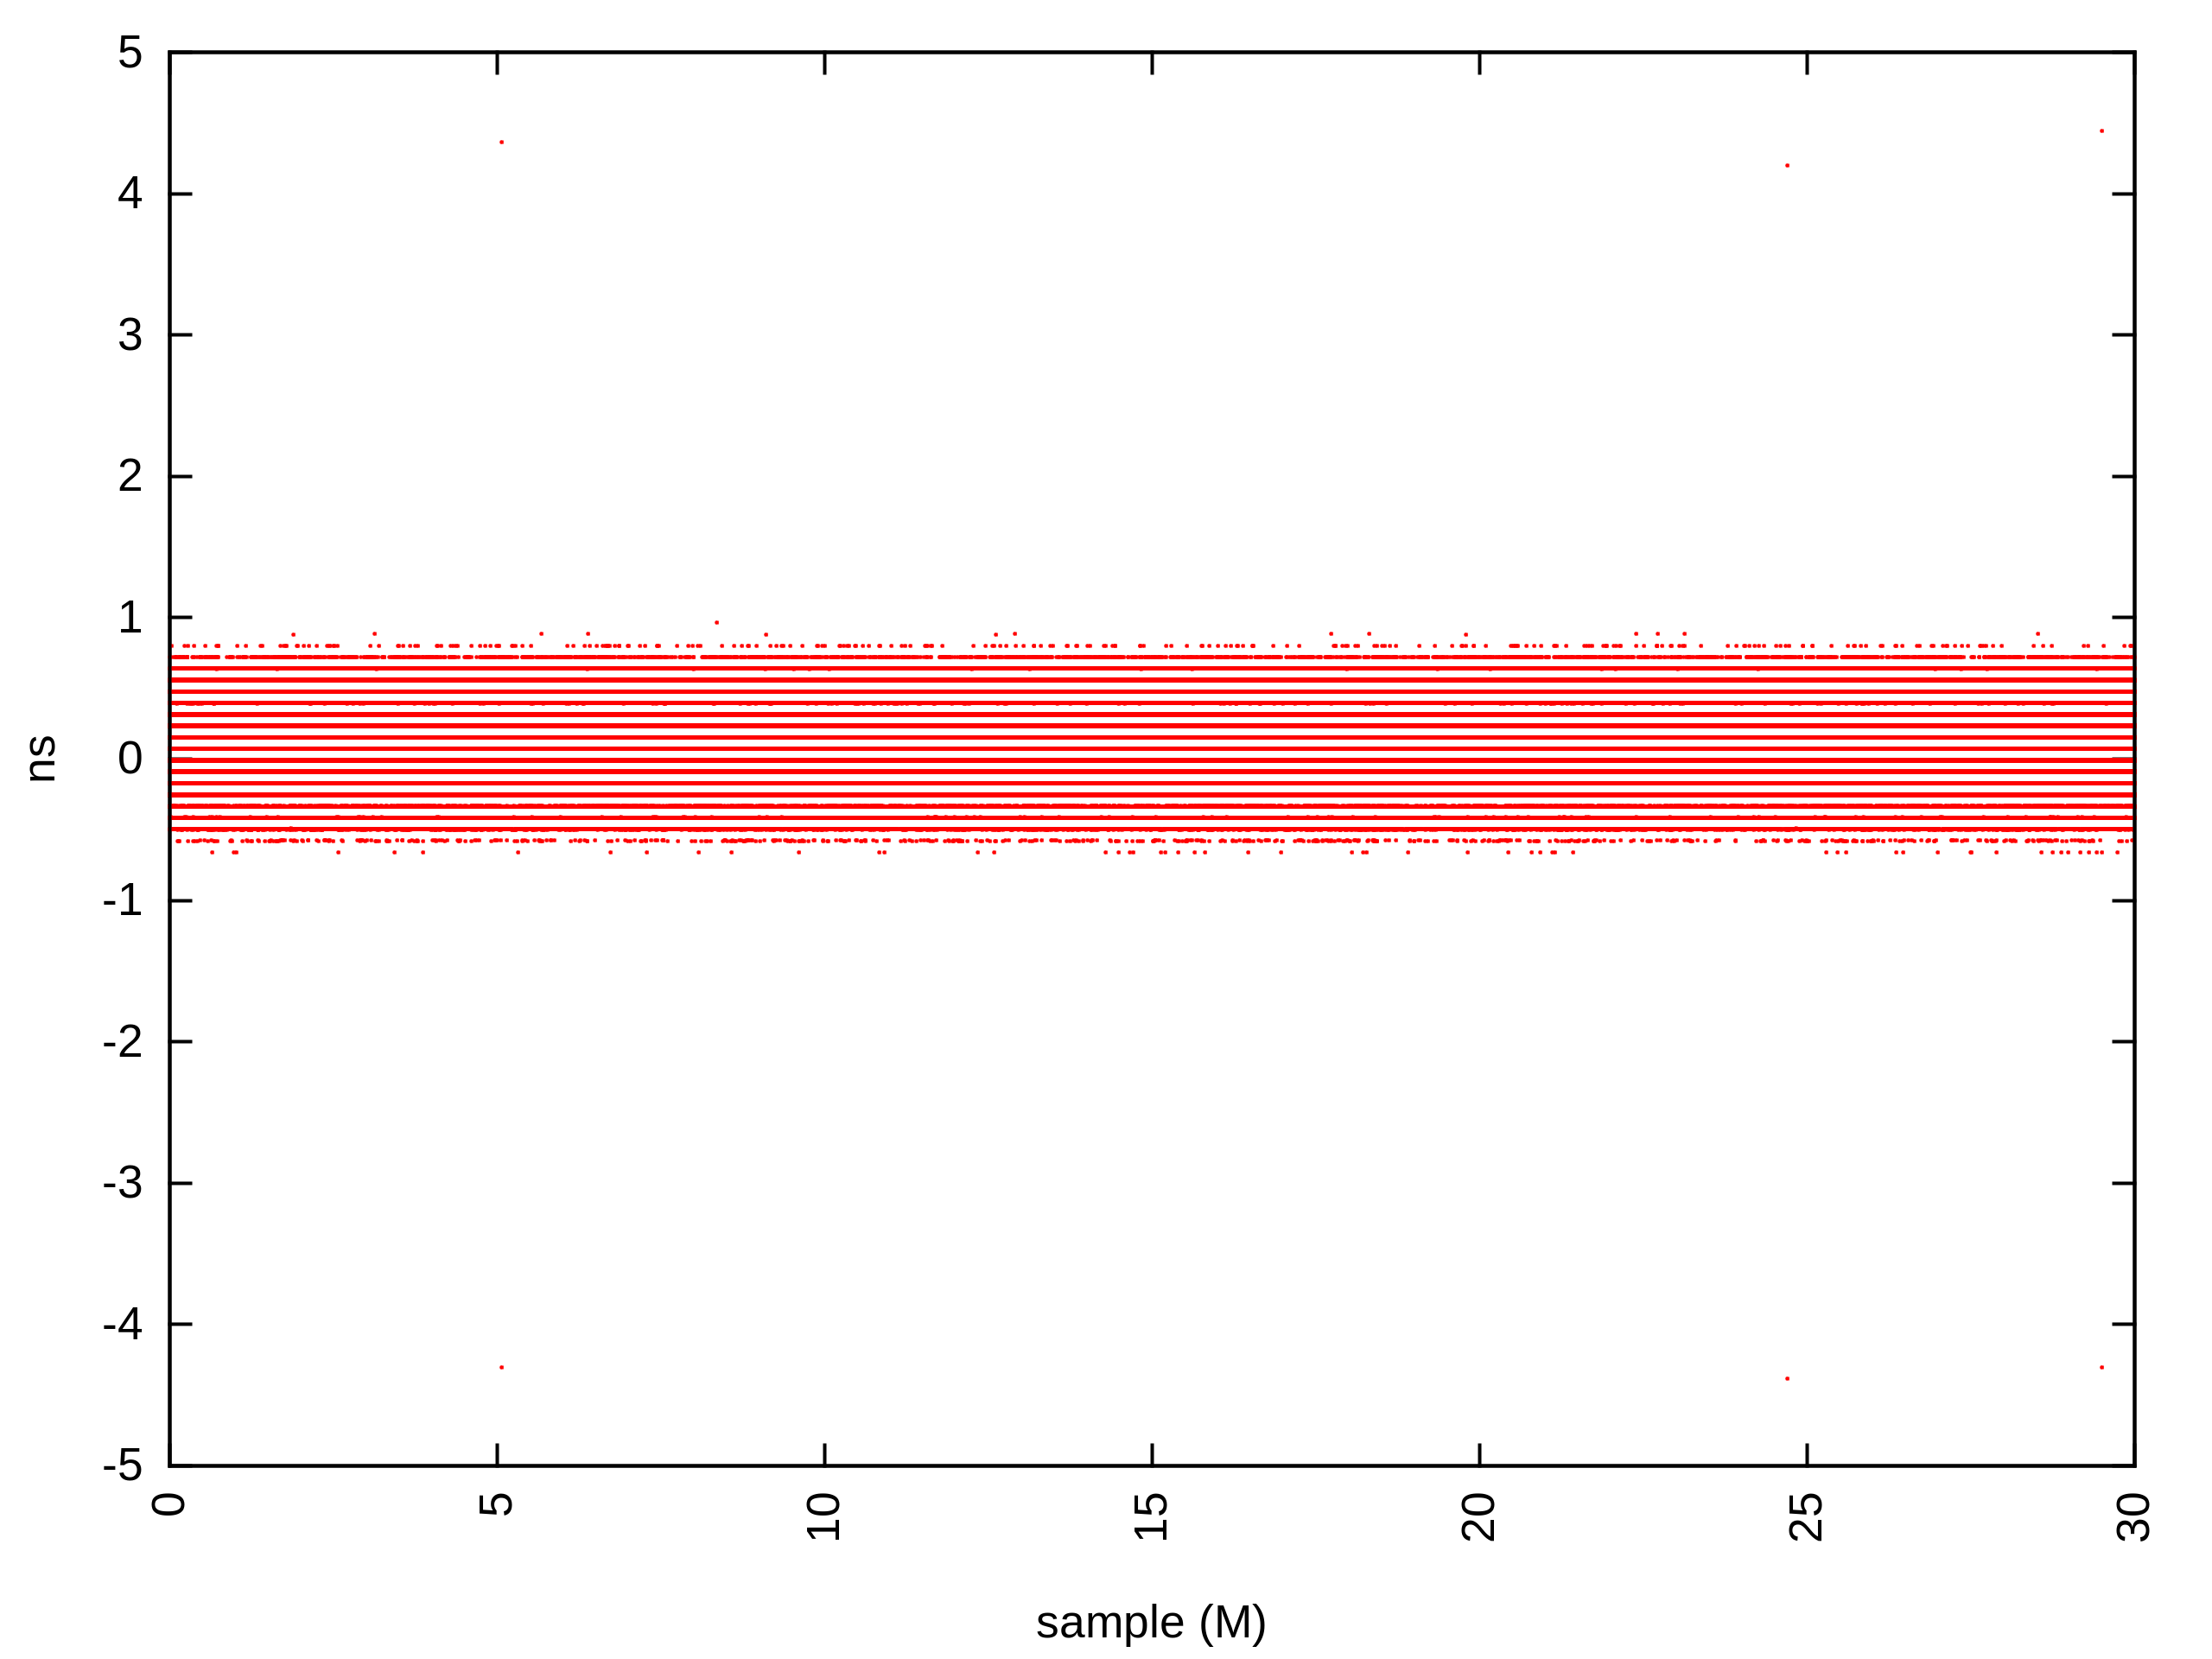
\includegraphics[width=0.9\textwidth]{img/test6_samples_relative.png}
  \caption{Test 6: Acquired samples (relative timestamps)}
  \label{test6_relative}
\end{figure}

\begin{figure}[ht!]
  \centering
  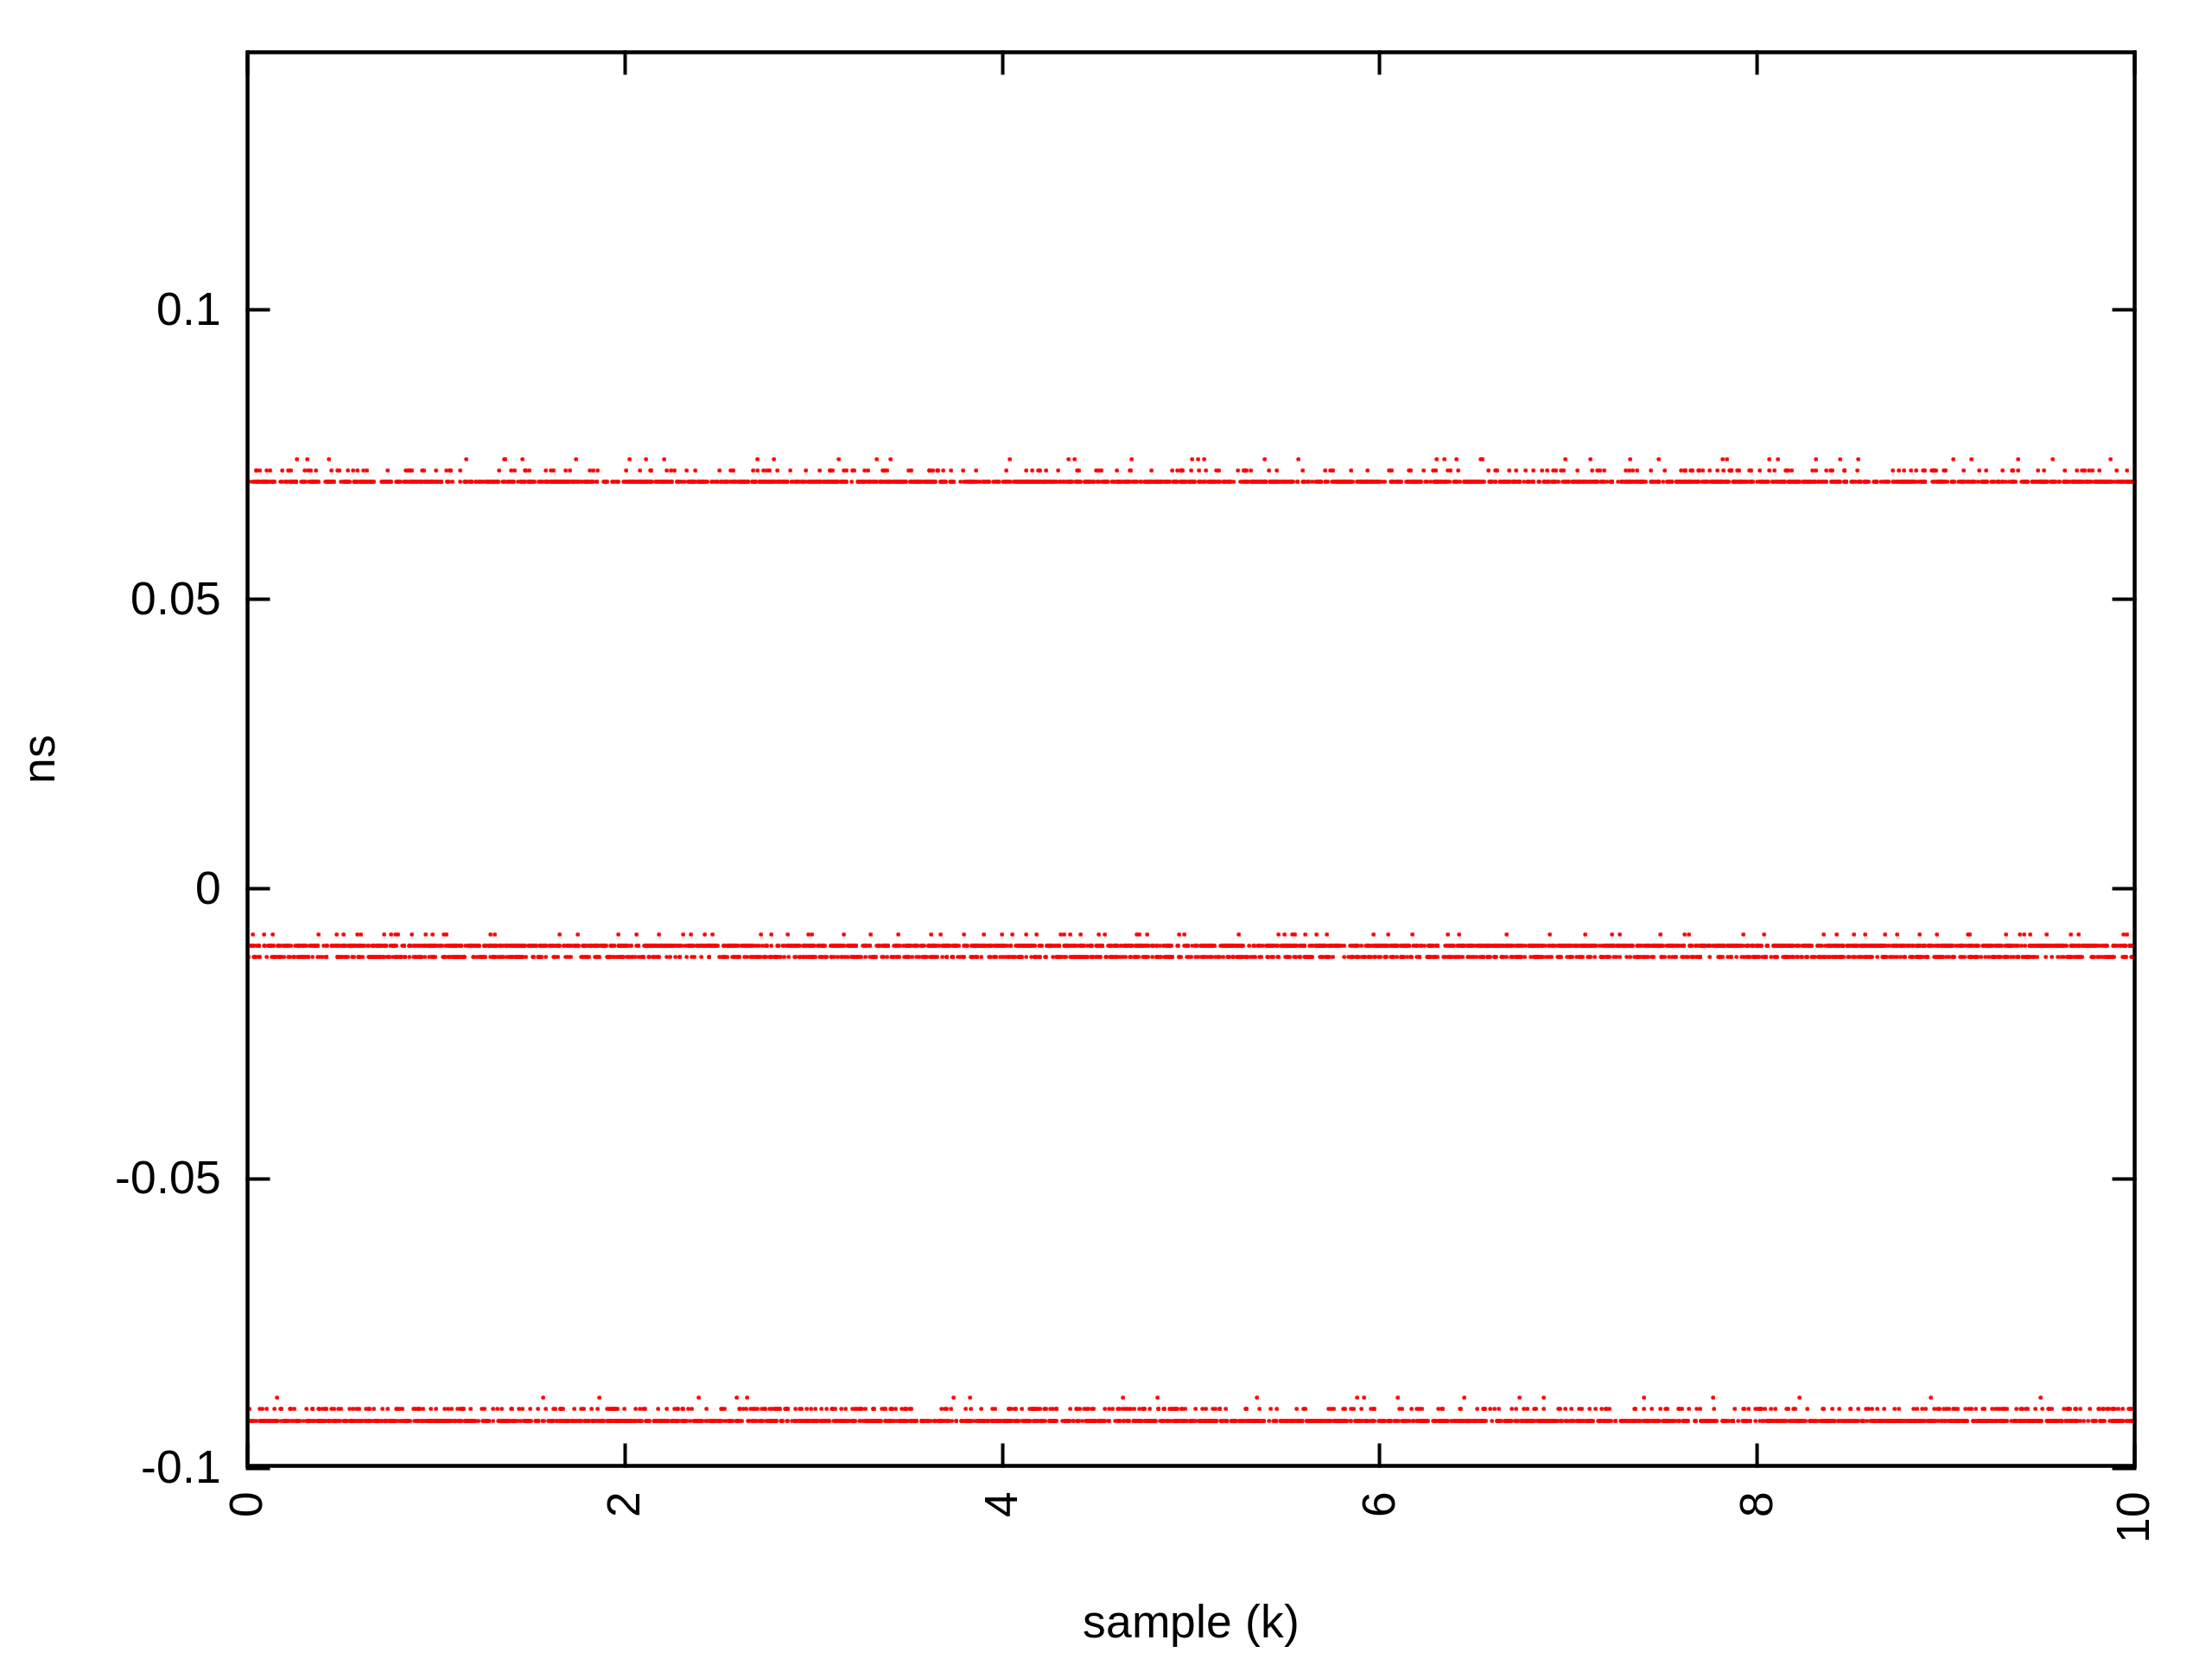
\includegraphics[width=0.7\textwidth]{img/test6_samples_relative_zoomxy.png}
  \caption{Test 6: Subset of acquired samples (relative timestamps)}
  \label{test6_relative_zoomy}
\end{figure}

The~Figure~\ref{test6_absolute} with absolute timestamps does not look like
an angled single line, similar to the~Figure~\ref{test5_absolute} with
absolute timestamps of the \textit{Test~5}. In the~Figure~\ref{test6_absolute}
samples draw many parallel horizontal lines. From the observation that samples
are visible as horizontal lines can be concluded that there is no drift between
clocks used on the pulse generator (Fine Delay) and the acquisition board (TDC).
Both used White Rabbit as the time reference.
It is believed that samples are spread into many parallel lines,
because of a precision limitation and a quantization effect of the timestamping
chip used on the TDC.
For an ideal chip, only one line would be present.

As seen on Figures~\ref{test6_absolute} and~\ref{test6_relative}, when
the White Rabbit is used, the comparison of relative and absolute timestamps
is not needed as both figures show similarities and no time drift is observed.

For figures with presented relative timestamps there is no visible difference
between results of \textit{Test~5} (Figure~\ref{test5_relative}) and
\textit{Test~6} (Figure~\ref{test6_relative}).

\FloatBarrier

\begin{figure}[ht!]
  \centering
  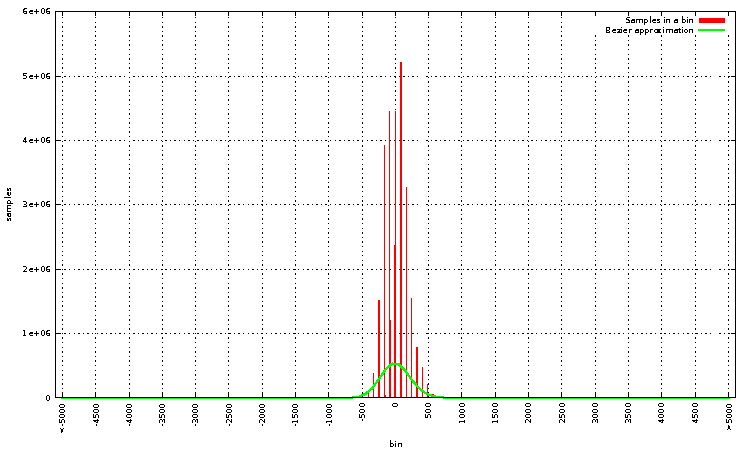
\includegraphics[width=0.80\textwidth]{img/test6_histogram.pdf}
  \caption{Test 6: Histogram of acquired samples (relative timestamps)}
  \label{test6_histogram}
\end{figure}

The same relative samples as above are
presented in the form of histogram in the~Figure~\ref{test2_histogram}.
Like in \textit{Test~5}, the histogram is divided into 1000 bins.
Each bin spans over 10 ps.
Two additional bins were added to keep all values greater and smaller than
5000ps.
Like for the other histogram,
the Bezier approximation has been added to the histogram figure.

\begin{figure}[ht!]
  \centering
  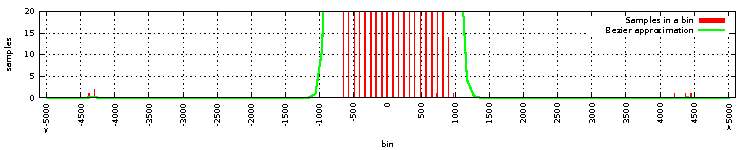
\includegraphics[width=1\textwidth]{img/test6_histogram_zoomy.pdf}
  \caption{Test 6: Histogram of acquired samples (relative timestamps)}
  \label{test6_histogram_zoomy}
\end{figure}

Figure~\ref{test6_histogram_zoomy} shows the zoom in on the Y axis of
the histogram presented in the~Figure~\ref{test6_histogram}.
This shows that bins outside the center part of the figure are empty
(with the exception of few samples around $\pm$4ns, but this problem is
discussed later).


\begin{figure}[ht!]
  \centering
  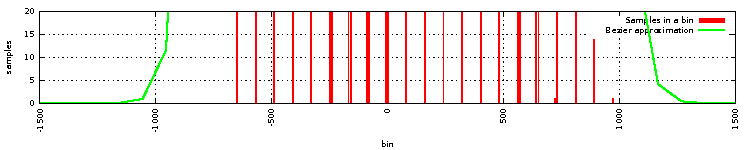
\includegraphics[width=1\textwidth]{img/test6_histogram_zoomx.pdf}
  \caption{Test 6: Histogram of acquired samples (relative timestamps),
           zoom in of the bottom center of the histogram
           (figure~\ref{test6_histogram})}
  \label{test6_histogram_zoomx}
\end{figure}


Figure~\ref{test6_histogram_zoomx} shows the zoom in of the bottom center
part of the histogram presented in the~Figure~\ref{test6_histogram}.
It gives better view about number of samples placed in bins that are close to
the center of the histogram.

\FloatBarrier

Statistical summary of several runs of the \textit{Test~6} is presented in
the Table~\ref{table_test6_summary}.

\begin{table}[!htb]
  \centering
  \footnotesize
  \begin{tabular}{|r|r|r|r|r|r|r|}
    \hline {\bf Run} & {\bf Data Volume} & {\bf Mean (ps)} & {\bf Sigma (ps)} & {\bf Min (ps)} & {\bf Max (ps)} & {\bf Range (ps)}  \\
    \hline
    1                & 30M               &              0  & 151.273          & -4466.797      & 4443.359       & 8910.156      \\
    **1              & 30M               &              0  & 151.256          &  -658.203      & 1044.922       & 1703.125      \\
    2                & 14M               &              0  & 152.660          & -4140.625      & 4119.141       & 8259.766      \\
    **2              & 14M               &              0  & 152.652          &  -660.156      &  884.766       & 1544.922      \\
    3                & 30M               &              0  & 152.931          & -4218.750      & 4443.359       & 8662.109      \\
    **3              & 30M               &              0  & 152.927          &  -660.156      &  962.891       & 1623.047      \\
    4                & 30M               &              0  & 156.481          & -4384.766      & 4445.312       & 8830.078      \\
    **4              & 30M               &              0  & 156.469          &  -658.203      &  964.844       & 1623.047      \\
    \hline
  \end{tabular}
  \caption{Summary of \textit{Test~6} runs}
  \label{table_test6_summary}
\end{table}


% 1:
% 0x5:2  3451189  0.07800054675585937902  0.00000000428125000000  0.00000000428125000000 seq: 3451189 timestamp: 1653616939.267000 raw: 6290312b:01fd435c:00000583, debug: 034a935a
% 0x5:2  3451190  0.07800054237109374511 -0.00000000438476562500 -0.00000000438476562500 seq: 3451190 timestamp: 1653616939.268001 raw: 6290312b:01ff2ba3:00000cbe, debug: 034a936a
% 0x5:2  5959102  0.07800054690820312775  0.00000000428320312500  0.00000000428320312500 seq: 5959102 timestamp: 1653619447.180001 raw: 62903af7:015752e4:000005d1, debug: 05aedbea
% 0x5:2  5959103  0.07800054244140625093 -0.00000000446679687500 -0.00000000446679687500 seq: 5959103 timestamp: 1653619447.181000 raw: 62903af7:01593b2b:00000ce2, debug: 05aedbfa
% 0x5:2 26440214  0.07800054674609374628  0.00000000428320312500  0.00000000428320312500 seq: 26440214 timestamp: 1653639928.292001 raw: 62908af8:022cf264:0000057e, debug: 1937216a
% 0x5:2 26440215  0.07800054244140625093 -0.00000000430468750000 -0.00000000430468750000 seq: 26440215 timestamp: 1653639928.293000 raw: 62908af8:022edaab:00000ce2, debug: 1937217a
% 0x5:2 28895436  0.07800054692773437937  0.00000000444335937500  0.00000000444335937500 seq: 28895436 timestamp: 1653642383.514001 raw: 6290948f:03d460d4:000005db, debug: 1b8e8cca
% 0x5:2 28895437  0.07800054246289062077 -0.00000000446484375000 -0.00000000446484375000 seq: 28895437 timestamp: 1653642383.515001 raw: 6290948f:03d6491b:00000ced, debug: 1b8e8cda

% 2:
% 0x5:2 6445883  0.58000053824999997509 -0.00000000414062500000 -0.00000000414062500000 seq: 6445883 timestamp: 1654051494.463001 raw: 6296d2a6:03731a7b:00000480, debug: 0625b3ba
% 0x5:2 6445884  0.58000054236914067030  0.00000000411914062500  0.00000000411914062500 seq: 6445884 timestamp: 1654051494.464000 raw: 6296d2a6:037502c3:00000cbd, debug: 0625b3ca

%3:
% 0x5:2 5255971  0.89500054680273433139  0.00000000444335937500  0.00000000444335937500 seq: 5255971 timestamp: 1654131572.866001 raw: 62980b74:0673c3d4:0000059b, debug: 0503323a
% 0x5:2 5255972  0.89500054258398442641 -0.00000000421875000000 -0.00000000421875000000 seq: 5255972 timestamp: 1654131572.867001 raw: 62980b74:0675ac1b:00000d2b, debug: 0503324a

% 4:
% 0x5:2  5073387  0.42800054674804688393  0.00000000436328125000  0.00000000436328125000 seq: 5073387 timestamp: 1654217901.815001 raw: 62995cad:06127d7c:0000057f, debug: 04d69eba
% 0x5:2  5073388  0.42800054244531249292 -0.00000000430273437500 -0.00000000430273437500 seq: 5073388 timestamp: 1654217901.816000 raw: 62995cad:061465c3:00000ce4, debug: 04d69eca
% 0x5:2 24693674  0.42800054659765623954  0.00000000420117187500  0.00000000420117187500 seq: 24693674 timestamp: 1654237522.102000 raw: 6299a952:00c28cf4:00000532, debug: 178cbaaa
% 0x5:2 24693675  0.42800054221289063339 -0.00000000438476562500 -0.00000000438476562500 seq: 24693675 timestamp: 1654237522.103001 raw: 6299a952:00c4753b:00000c6d, debug: 178cbaba
% 0x5:2 29494503  0.42800054695312500508  0.00000000444531250000  0.00000000444531250000 seq: 29494503 timestamp: 1654242322.931000 raw: 6299bc12:06efbe1c:000005e8, debug: 1c20ce7a
% 0x5:2 29494504  0.42800054264843750973 -0.00000000430468750000 -0.00000000430468750000 seq: 29494504 timestamp: 1654242322.932001 raw: 6299bc12:06f1a663:00000d4c, debug: 1c20ce8a

Like in previous tests, in the runs there were relative samples that
significantly differed from other values.
As mentioned before, it is suspected that this is the same issue
as described in~\cite{tdc_perf_test}.
The table~\ref{table_test6_summary}
includes the calculations for the same runs (marked with asterisk),
but without suspected timestamps. The Table~\ref{table_test6_samples_excluded}
includes the details about the excluded values.


The mean value of samples gathered in each run is very close to 0.
This proves that the time drift (thanks to White Rabbit) between
the pulse generator and the acquisition board is very small.

Other values like Sigma, Minimum, Maximum and Range are very similar to
the values included in the similar table for other test e.g. \textit{Test~5}
(Table~\ref{table_test5_summary}).
\begin{table}[!htb]
\centering
\tiny
  \begin{tabular}{|r|r|r|}
    \hline
    {\bf run } &{\bf sample \#} & {\bf Delta (ps)} \\
    \hline
    1          &  3451189  &  4281.250000 \\
    1          &  3451190  & -4384.765625 \\
    1          &  5959102  &  4283.203125 \\
    1          &  5959103  & -4466.796875 \\
    1          & 26440214  &  4283.203125 \\
    1          & 26440215  & -4304.687500 \\
    1          & 28895436  &  4443.359375 \\
    1          & 28895437  & -4464.843750 \\
    2          &  6445883  & -4140.625000 \\
    2          &  6445884  &  4119.140625 \\
    3          &  5255971  &  4443.359375 \\
    3          &  5255972  & -4218.750000 \\
    4          &  5073387  &  4363.281250 \\
    4          &  5073388  & -4302.734375 \\
    4          & 24693674  &  4201.171875 \\
    4          & 24693675  & -4384.765625 \\
    4          & 29494503  &  4445.312500 \\
    4          & 29494504  & -4304.687500 \\
    \hline
  \end{tabular}
  \caption{Samples excluded from calculations of \textit{Test~6} runs}
  \label{table_test6_samples_excluded}
\end{table}

To gather all data in the described test, the following python command has been
used:
\begin{lstlisting}
$ python -d -m pytest --usr-acq-count=100000000 --usr-acq-period-ns=1000000 \
  test_fmctdc_acquisition.py::TestFmctdcAcquisition::test_acq_timestamp_multiple_hist \
  --tdc-id-ch 0x5:2 --histogram-file test6_hist --bin-min-ps -5000 --bin-max-ps 5000 \
  --bins-num 1000 --samples-file test6 --tdc-wr-on
\end{lstlisting}

\FloatBarrier

% ##########################################################################
\section{Maximum sample rates}
\label{performance}

To find the maximum sample rate that FMC TDC can handle on SPEC\cite{SPEC}
and SVEC\cite{SVEC} boards,
two tests written in pytest\cite{pytest} were used:
\begin{itemize}
  \item \texttt{test\_acq\_timestamp\_multiple\_hist} -- Pytest test that is
    capable of saving to the disk samples and histogram data.
    It can save acquisition data for one or more channels at the same time.
  \item \texttt{test\_acq\_performance} -- Pytest test written to check
    the maximum rate of samples that can be handled on a system.
    To reduce the number of required computations it only checks the sequence
    number of sample to detect missed samples. This test is not capable
    to save any information about the content of the received samples.
\end{itemize}

To find the maximum stable sample rate that can be handled the number of tests
were performed. The summary is presented in the table~\ref{max_sample_rate}.
\begin{table}[htbp]
% \begin{center}
\centering
\footnotesize
  \begin{tabular}{|l|r|r|}
    \hline {\bf Test description} & {\bf SPEC (kHz)} & {\bf SVEC (kHz)}  \\
    \hline
    Optimized test (\texttt{test\_acq\_performance}) &               200.0 & \textasciitilde83.3 \\
    Only receive samples                             & \textasciitilde90.9 & \textasciitilde44.4 \\
    Save histogram data                              &                20.0 &                 8.0 \\
    Save samples data                                &  \textasciitilde6.6 &  \textasciitilde3.0 \\
    Save samples and histogram data                  &                 5.0 &                 2.0 \\
    \hline
  \end{tabular}
  \caption{Approximate maximum sample rate}
  \label{max_sample_rate}
% \end{center}
\end{table}

The aim of the first test (Optimized test (\texttt{test\_acq\_performance}))
listed in the table~\ref{max_sample_rate} is to determine the maximum
sample rate that can be handled. To achieve this, the optimized test script
has been prepared with the only minimal computation done to the samples.
It included only the check if acquired samples are in sequence.

The second row includes non-optimized test that acquired incoming samples.
Maximum stable sample rate is about half of the first test.

The next test analyzes every single timestamp of incoming sample and places
the timestamp in a proper histogram's data bin.

The forth test additionally stores timestamps in a test file on a file system.

The last test does both, it stores information needed for histogram calculation
and stores timestamps in a test file on a file system.

When finding the maximum sample rate, it was observed that the limiting factor
was the CPU's computing power.
The machine used for SPEC testing is based on Intel Core i5-8500\cite{spec.cpu}
CPU.
It has 6-cores, no hyper-threading, with base frequency 3GHz, maximum 4.1GHz.
On the contrary, the machine used for SVEC testing is based on
Intel Pentium D1519\cite{svec.cpu} CPU.
It has 4-cores with hyper-threading, with base frequency 1.5GHz, maximum 2.1GHz.

The difference in CPU performance can explain the gap between
the maximum achieved sample rate with SPEC and SVEC during the testing.
The maximum throughput of PCIe (hundreds of MB/s) is much higher comparing to
VME (tens of MB/s).
However, it was not observed that the VME performance was the limiting factor
for the test results.

It is believed that higher performance may be achieved for SPEC and SVEC, when
the more powerful CPU is used. The numbers gathered in the
table~\ref{max_sample_rate} above may be influenced by many factors e.g.~the
CPU load.
On the other hand, there are a number of ways to improve the number of samples
that the system can handle, e.g.~by using multi-threaded application.

% ##########################################################################
\subsection{SPEC}
\label{perf_spec}

The machine used for SPEC testing is based on Intel Core i5-8500\cite{spec.cpu}
CPU.
It has 6-cores, no hyper-threading, with base frequency 3GHz, maximum 4.1GHz.

The maximum stable sample rate achieved using optimized test
(\texttt{test\_acq\_performance}) is
about 200kHz. The following command has been used:
\begin{lstlisting}
$ python -d -m pytest  --usr-acq-count=10000000 --usr-acq-period-ns=5000 \
  test_fmctdc_acquisition.py::TestFmctdcAcquisition::test_acq_performance \
  --tdc-id-ch 0x18:1 --fd-id-ch 0x1a:1
\end{lstlisting}

The test without saving samples nor histogram data was able to handle samples
with the rate about 90kHz.
The following command has been used:
\begin{lstlisting}
$ python -d -m pytest  --usr-acq-count=10000000 --usr-acq-period-ns=11000 \
  test_fmctdc_acquisition.py::TestFmctdcAcquisition::test_acq_timestamp_multiple_hist \
  --tdc-id-ch 0x18:1 --fd-id-ch 0x1a:1
\end{lstlisting}

The test with histogram calculation only was able to handle samples with the
rate about 20kHz. The following command has been used:
\begin{lstlisting}
$ python -d -m pytest  --usr-acq-count=10000000 --usr-acq-period-ns=51000 \
  test_fmctdc_acquisition.py::TestFmctdcAcquisition::test_acq_timestamp_multiple_hist \
  --tdc-id-ch 0x18:1 --fd-id-ch 0x1a:1 --histogram-file=hist.txt --bin-min-ps -5000 \
  --bin-max-ps 5000 --bins-num 1000
\end{lstlisting}

The test with sample store only was able to handle samples with the
rate about 6.6kHz. The following command has been used:
\begin{lstlisting}
$ python -d -m pytest  --usr-acq-count=10000000 --usr-acq-period-ns=150000 \
  test_fmctdc_acquisition.py::TestFmctdcAcquisition::test_acq_timestamp_multiple_hist \
  --tdc-id-ch 0x18:1 --fd-id-ch 0x1a:1 --samples-file=sample.txt
\end{lstlisting}

The test with both, storing samples and histogram data was able to handle
samples with the rate about 5kHz. The following command has been used:
\begin{lstlisting}
$ python -d -m pytest  --usr-acq-count=10000000 --usr-acq-period-ns=200000 \
  test_fmctdc_acquisition.py::TestFmctdcAcquisition::test_acq_timestamp_multiple_hist \
  --tdc-id-ch 0x18:1 --fd-id-ch 0x1a:1 --samples-file=sample.txt  --bin-min-ps -5000 \
  --bin-max-ps 5000 --bins-num 1000 --histogram-file=hist.txt
\end{lstlisting}


% ##########################################################################
\subsection{SVEC}
\label{perf_svec}

The machine used for SVEC testing is based on
Intel Pentium D1519\cite{svec.cpu} CPU.
It has 4-cores with hyper-threading, with base frequency 1.5GHz, maximum 2.1GHz.

The maximum stable sample rate achieved using optimized test
(\texttt{test\_acq\_performance}) is
about 83,3kHz. The following command has been used:
\begin{lstlisting}
$ pthon -d -m pytest  --usr-acq-count=10000000 --usr-acq-period-ns=12000 \
  test_fmctdc_acquisition.py::TestFmctdcAcquisition::test_acq_performance \
  --tdc-id-ch 0x5:2 --fd-id-ch 0x1a:1
\end{lstlisting}

The test without saving samples nor histogram data was able to handle samples
with the rate about 45kHz.
The following command has been used:
\begin{lstlisting}
$ python -d -m pytest  --usr-acq-count=10000000 --usr-acq-period-ns=22500 \
  test_fmctdc_acquisition.py::TestFmctdcAcquisition::test_acq_timestamp_multiple_hist \
  --tdc-id-ch 0x5:2 --fd-id-ch 0x1a:1
\end{lstlisting}

The test with only histogram calculation was able to handle samples with the
rate about 8kHz. The following command has been used:
\begin{lstlisting}
$ python -d -m pytest  --usr-acq-count=10000000 --usr-acq-period-ns=125000
  test_fmctdc_acquisition.py::TestFmctdcAcquisition::test_acq_timestamp_multiple_hist \
  --tdc-id-ch 0x5:2 --fd-id-ch 0x1a:1 --histogram-file=hist.txt --bin-min-ps -5000 \
  --bin-max-ps 5000 --bins-num 1000
\end{lstlisting}

The test with only sample store was able to handle samples with the
rate about 3kHz. The following command has been used:
% but it is probably too much for longer periods
\begin{lstlisting}
$ python -d -m pytest  --usr-acq-count=10000000 --usr-acq-period-ns=330000 \
  test_fmctdc_acquisition.py::TestFmctdcAcquisition::test_acq_timestamp_multiple_hist \
  --tdc-id-ch 0x5:2 --fd-id-ch 0x1a:1 --samples-file=sample.txt
\end{lstlisting}

The test with both, storing samples and histogram data was able to handle
samples with the rate about 2kHz. The following command has been used:
\begin{lstlisting}
$ python -d -m pytest  --usr-acq-count=10000000 --usr-acq-period-ns=500000 \
  test_fmctdc_acquisition.py::TestFmctdcAcquisition::test_acq_timestamp_multiple_hist \
  --tdc-id-ch 0x5:2 --fd-id-ch 0x1a:1 --samples-file=sample.txt  --bin-min-ps -5000 \
  --bin-max-ps 5000 --bins-num 1000 --histogram-file=hist.txt
\end{lstlisting}

% ##########################################################################
\section{Summary}
\label{Summary}
The results presented in this report are in line with the results presented
in previous reports (\cite{tdc_perf_test}, \cite{tdc_precision_test}
and~\cite{tdc_long_runs}) done for older releases.

The tests shows that use of White Rabbit with its common notion of time
can improve long term stability of results and avoid the drift of local
oscillators.

The issue of the $\pm$ 4ns spikes with 1 wrong timestamp every few millions
as described in older reports (\cite{tdc_perf_test}, \cite{tdc_precision_test}
and~\cite{tdc_long_runs}) sill exists.

% ##########################################################################
% ##########################################################################

\begin{thebibliography}{99}
\bibitem{tdc.release}
TDC FMC Release 8.0 website,  \url{https://ohwr.org/project/fmc-tdc/wikis/release-v8}

\bibitem{tdc}
TDC FMC website,  \url{https://ohwr.org/project/fmc-tdc/wikis}

\bibitem{SPEC}
Simple PCIe FMC carrier (SPEC) website,  \url{https://ohwr.org/project/spec/wikis/home}

\bibitem{SVEC}
Simple VME FMC carrier (SVEC) website,  \url{https://ohwr.org/project/svec/wikis/home}

\bibitem{pytest}
pytest 6.2.5, 2004
Krekel et al., \url{https://github.com/pytest-dev/pytest}

\bibitem{spec.cpu}
Intel Core i5-8500 specification website,\\
\url{https://ark.intel.com/content/www/pl/pl/ark/products/129939/intel-core-i58500-processor-9m-cache-up-to-4-10-ghz.html}

\bibitem{a25}
VME Single Computer Board Duagon A25, https://www.duagon.com/products/details/a25/

\bibitem{svec.cpu}
Intel Pentium D1519 specification website,\\
\url{https://ark.intel.com/content/www/pl/pl/ark/products/91559/intel-pentium-processor-d1519-6m-cache-1-50-ghz.html}

\bibitem{tdc_perf_test}
TDC mezzanine board, Performance testing. E. Gousiou,
\url{https://www.ohwr.org/project/fmc-tdc/uploads/5bf6bf0a2d633382987f09a0915e20d8/TDCperformance.pdf}

\bibitem{tdc_precision_test}
Results of the Precision tests on the TDC mezzanine board. E. Gousiou,\\
\url{https://www.ohwr.org/project/fmc-tdc/uploads/a3b1bc0987d7cd2290d3394d73d835c8/TDCprecision.pdf}

\bibitem{tdc_long_runs}
TDC mezzanines on SVEC carriers Long Runs. E. Gousiou,
\url{https://www.ohwr.org/project/fmc-tdc/uploads/b08624193e2e48947a11708639d96921/LongRunsOnSVEC.pdf}
\end{thebibliography}
\end{document}
